\documentclass[12pt]{report}
\usepackage[Glenn]{fncychap}
\usepackage[T1]{fontenc}
%\usepackage[french]{babel}
\usepackage[francais]{babel}
\usepackage{breakcites}
\usepackage{slashbox}
%\usepackage{fontspec}
\usepackage{wrapfig}
\usepackage{graphicx}
\usepackage{soul}
\usepackage{url}
\usepackage[colorlinks=true, linkcolor=black, urlcolor=black, citecolor=black]{hyperref}
% \usepackage[hyphens, spaces, obeyspaces]{url}
\usepackage[a4paper, width=150mm, top=25mm, bottom=25mm]{geometry}
\usepackage{parskip}
\usepackage{enumitem}
\usepackage{titlesec}
\usepackage{listings}
\usepackage{placeins}
\usepackage{float}
\restylefloat{table}
\usepackage[final]{pdfpages}
\usepackage{xcolor}
\usepackage{tocbibind}
\usepackage{tocloft}
\usepackage[utf8]{inputenc}
\usepackage{xpatch}
\usepackage{amsmath}
\usepackage{amsthm}
\usepackage{amsfonts}
\usepackage{graphics}
\usepackage{color}
% \usepackage[grey,utopia]{quotchap}
\usepackage{moreverb}
\usepackage{xcolor}
\usepackage{framed}
\usepackage[algo2e, french, onelanguage, ruled]{algorithm2e}
\usepackage{titling}
\setlist[itemize]{label=\textbullet}
\usepackage{fancyhdr}
\pagestyle{fancy}   
\fancyhead{}
\fancyhead[C]{\leftmark}
\renewcommand{\headrulewidth}{0.4pt}
\renewcommand{\footrulewidth}{0.4pt}
\usepackage{xcolor}
\definecolor{light-gray}{gray}{0.90}
\newcommand{\code}[1]{\colorbox{light-gray}{\texttt{#1}}}
\usepackage{listings}
\usepackage{multirow}
\usepackage{makecell}
\usepackage{algorithm}
\usepackage[noend]{algpseudocode}
\renewcommand\theadalign{bc}
\renewcommand\theadfont{\bfseries}
\renewcommand\theadgape{\Gape[4pt]}
\renewcommand\cellgape{\Gape[4pt]}
\usepackage[dvipsnames]{xcolor}
\setlength{\textfloatsep}{0.1cm}
\usepackage{tcolorbox}
\usepackage{tablefootnote}

\renewcommand{\thesubsubsection}{\thesubsection.\arabic{subsubsection}}
\setcounter{tocdepth}{3}
\setcounter{secnumdepth}{3}

%\setcounter{tocdepth=3}{3n}
%\setcounter{secnumdepth}{4}
\usepackage[utf8x]{inputenc}
\usepackage{arabtex}
\usepackage{utf8}
\usepackage{pifont}
\setcode{utf8}
\addto{\captionsfrench}{\renewcommand{\abstractname}{\RL{ملخص}}}
\usepackage{array}
\newcolumntype{L}[1]{>{\raggedright\let\newline\\\arraybackslash\hspace{0pt}}m{#1}}
\newcolumntype{C}[1]{>{\centering\let\newline\\\arraybackslash\hspace{0pt}}m{#1}}
\newcolumntype{R}[1]{>{\raggedleft\let\newline\\\arraybackslash\hspace{0pt}}m{#1}}
\newcolumntype{M}[1]{>{\centering\arraybackslash}m{#1}}
\usepackage{longtable}
\lstdefinestyle{code}{
language=python,                   
keywordstyle=\color{blue},      
stringstyle=\color{blue},        
commentstyle=\color{gray},     
basicstyle=\small\ttfamily,           
numbers=left,                   
numberstyle=\normalsize,        
numbersep=7pt,                  
showstringspaces=false,         
breaklines=true,                
frame=leftline,                 
framerule=2pt,
}

\lstdefinestyle{api}{
language=python,                   
keywordstyle=\color{blue},      
stringstyle=\color{blue},        
commentstyle=\color{gray},     
basicstyle=\small\ttfamily,           
% numbers=false,                   
numberstyle=\normalsize,        
numbersep=7pt,                  
showstringspaces=false,         
breaklines=true,                
frame=leftline,                 
framerule=2pt,
}

\usepackage{color, colortbl}
\definecolor{Gray}{gray}{0.6}
\newcommand{\ie}{\textit{i}.\textit{e}., }
%~~~BEGIN~~~%
\begin{document}

\newpage
\setlength{\parindent}{0.5cm}

%%% Cover Page %%%

\includepdf[pages=1]{other/cover.pdf} 

%%% Content tables %%% 
\pagenumbering{gobble}
\addtocontents{toc}{\protect\setcounter{tocdepth}{2}}
\renewcommand{\contentsname}{Sommaire}
\tableofcontents
\clearpage


\listoffigures
\clearpage

\listoftables
\clearpage

 \listofalgorithmes
\clearpage

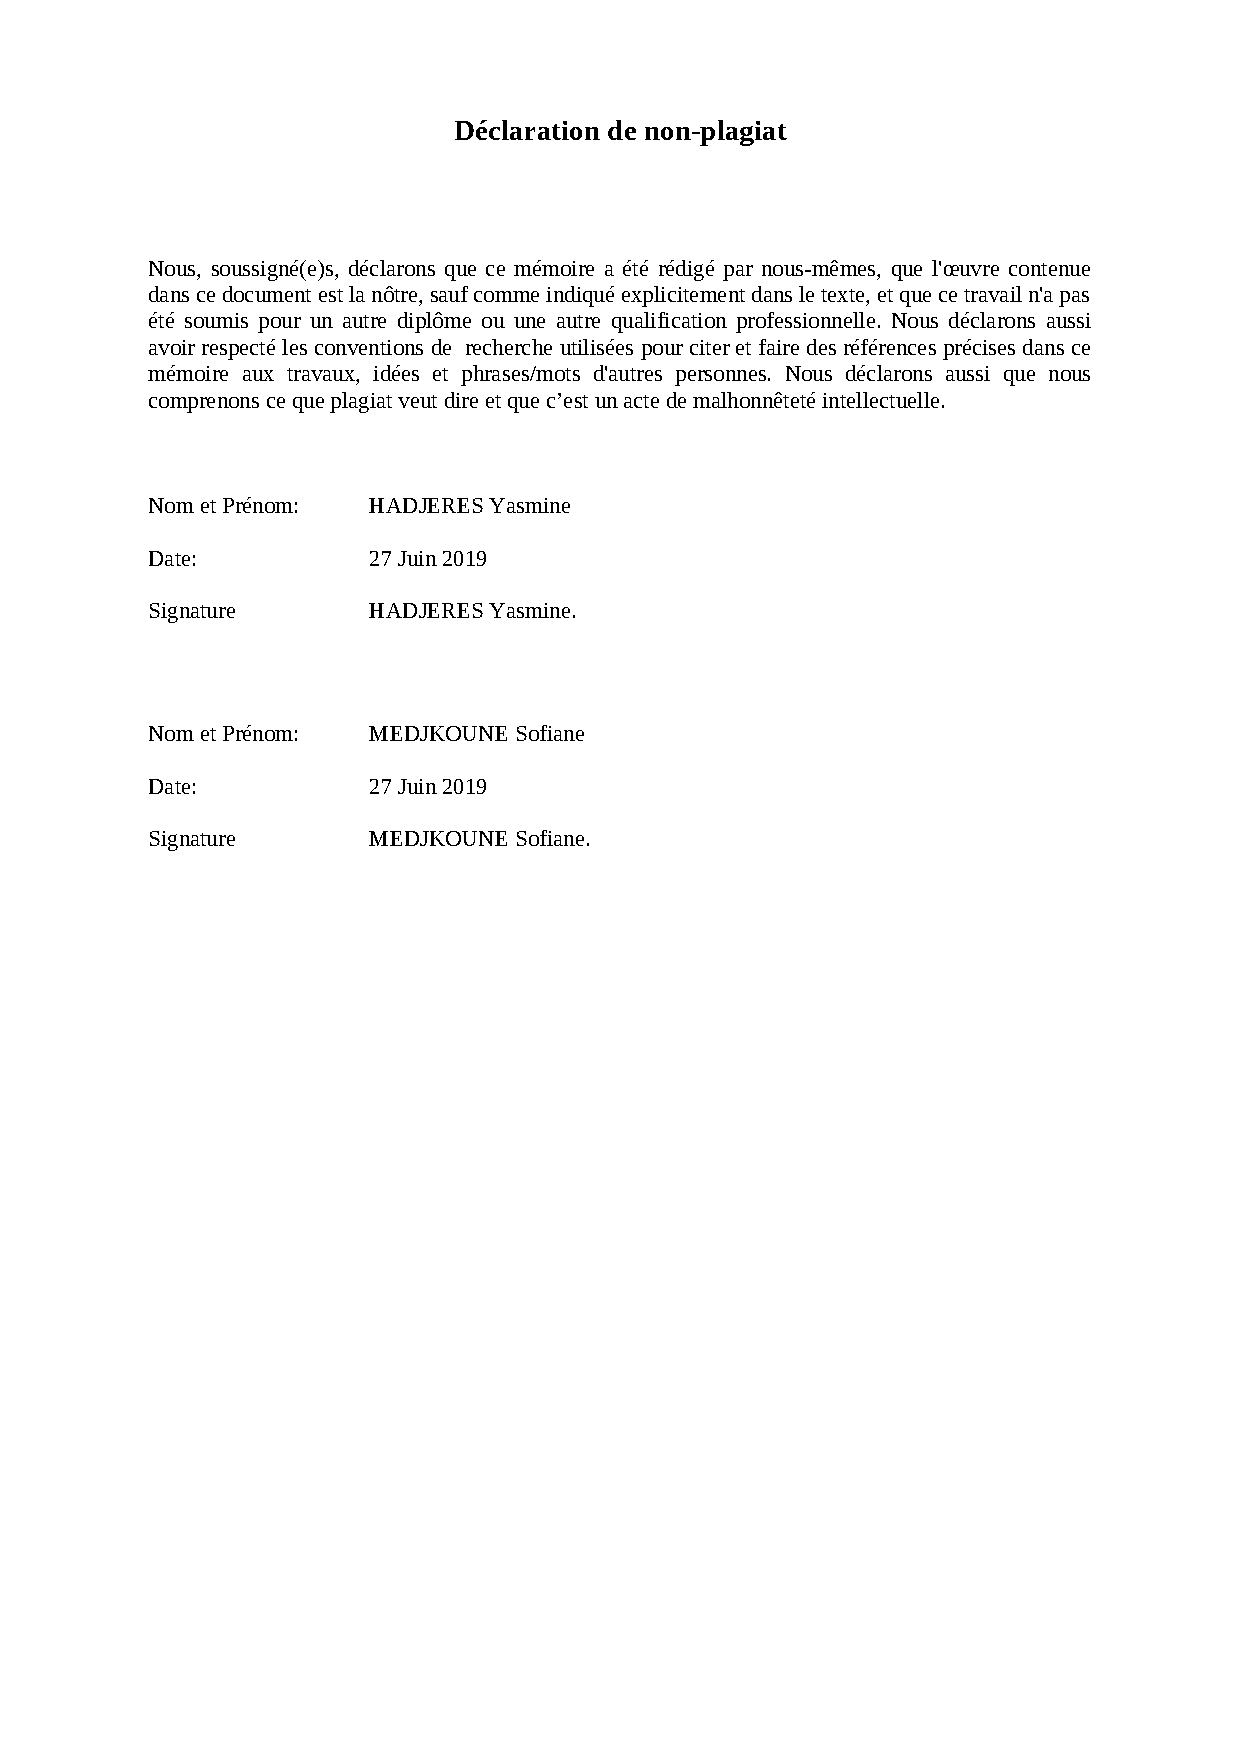
\includepdf[pages=1]{other/declaration_plagiat.pdf}
\chapter*{Remerciements} % Ne numérote pas le chapitre

Nous commençons par adresser nos remerciements à Dieu le miséricordieux qui nous a donné la force, la patience, le courage et tous les moyens pour mener à terme notre projet de fin d'études. \\

\textbf{À notre encadreur : Professeur Ahmed Guessoum}
\\

Tous nos remerciements vont vers vous, professeur Ahmed Guessoum. D’abord pour la qualité des enseignements techniques et humains que vous avez su nous transmettre ces deux dernières années. Nous vous remercions pour la bienveillance, la patience, les remarques précieuses ainsi que la multitude de conseils que vous nous avez donnés durant toute la période de ce projet de fin d’études. Pour finir, merci pour la chance que vous nous avez donnée de travailler à vos côtés.
\\

\textbf{À notre co-encadreur : Mademoiselle Asma Aouichat}
\\

Nous avons eu l’honneur de travailler à vos côtés durant tout un semestre. Votre gentillesse, votre compréhension et votre disponibilité ont toujours suscité notre admiration. Veuillez bien recevoir nos remerciements les plus distincts. \\

\textbf{Aux membres du jury} \\

Un grand merci au professeur F. KHELLAF que nous avons l'honneur d'avoir comme présidente du jury ainsi qu'a Mme M. DJEFFAL, membre du jury. Merci à vous de prendre le temps d'étudier notre travail et de le critiquer. \\ \\
Enfin, nous tenons à remercier toutes les personnes qui nous ont aidé de près ou de loin à la réalisation de ce modeste travail. 


\chapter*{Dédicaces} % Ne numérote pas le chapitre

Je dédie ce projet de fin d'études à, 

Mes chers parents, qui m'ont donné la force et le courage de les rendre fiers. Que Dieu vous protège et vous donne tout le bonheur du monde. \\ \\
Ma petite soeur et à mes grands parents. \\ \\
Tous mes amis et plus particulièrement Nazime, Yasser, Anas, Anaïs, Anis, Lilia, Ramzi, Wissam, Massil, Medina, Adel, Ghiles, Naila.\\ \\
La famille Open Minds Club, vous n'avez pas idée de ce que vous m'avez apporté.\\ \\
Vous êtes les personnes à qui je tiens le plus, j'espère vous garder près de moi. Merci. \\ \\

\vspace{0.5cm}
\begin{center}
\Large
\hspace{12.5cm}
\textbf{Sofiane}
\end{center}

\chapter*{Dédicaces} % Ne numérote pas le chapitre

Je dédie ce travail à :

Ma famille en commençant par mes chers parents, mon mari, mon frère, mes grands parents et ma belle famille, que Dieu vous garde tous pour moi.

À tous mes amis en commençant par : Hadia, Chanez, Lilia, Naila, Fida, Salim, Sofiane (C), Nadjib.
 \\

\vspace{0.5cm}
\begin{center}
\Large
\hspace{12.5cm}
\textbf{Yasmine}
\end{center}

\newpage    

%%% Chapters %%%
\pagenumbering{arabic}

% \chapter*{Introduction Générale}
\chapter*{Introduction} % Ne numérote pas le chapitre
\addcontentsline{toc}{chapter}{Introduction générale} % Référence l'introduction dans la table des matières
\chaptermark{Introduction générale}
L'intelligence artificielle (IA) vise à permettre aux machines d'émuler l'intelligence humaine. Cette branche de l'informatique inclut l’apprentissage, le raisonnement et l’auto-correction. L'intelligence artificielle, au fil des décennies, a révolutionné différents domaines en passant par la vision artificielle, les systèmes experts et le traitement automatique du langage naturel (TALN) afin de rendre les interactions entre l'homme et la machine plus naturelles. Depuis le début des années 1960s, plusieurs applications de TALN commencèrent à voir le jour à savoir, la traduction automatique, les systèmes de questions-réponses, mais aussi, les systèmes de reconnaissance de la parole. 

La reconnaissance de la parole a suscité un grand engouement que ce soit dans le domaine de la recherche ou dans le domaine multimédia. À ce jour, toutes les grandes compagnies comme Google, Apple, Facebook, Amazon ou Microsoft travaillent activement sur l'amélioration des technologies du traitement automatique de la parole afin d'offrir une meilleure interaction avec leurs produits. Cependant, une mauvaise reconnaissance peut mener à une mauvaise communication de l'information, une perte de temps et une frustration de l'utilisateur. Le monde arabe, et les arabophones plus particulièrement, ne disposent pas d'outils de reconnaissance de la parole aussi performants que ceux qui existent pour d'autres langues comme l'anglais. Ceci pose donc le défi d'améliorer ces outils pour la langue arabe. 

Il est clair que de nos jours, les systèmes de reconnaissance de la parole pour les langues étrangères, et notamment l'anglais, ont atteint des niveaux de fiabilité très intéressants. Ceci n'est malheureusement pas encore le cas pour la langue arabe qui présente des résultats nettement moins satisfaisants. Cette modeste performance est due au manque de corpus assez riches, mais aussi due à la complexité morphosyntaxique de la langue arabe par rapport aux autres langues. Le constat n'est cependant pas que négatif car, aujourd'hui, plusieurs équipes de recherches et entreprises travaillent sur l'amélioration de ces systèmes. Il y a eu également l'introduction de nouvelles techniques en matière d'apprentissage profond qui permettent de tirer plus facilement profit des corpus de dialogue en arabe et, ainsi, d'outrepasser la complexité de la langue. 
\newpage
Notre travail s'inscrit dans le cadre d'un projet de recherche. Dans l'optique de contribuer à l'amélioration des technologies du traitement automatique de la parole, nous avons développé un système de reconnaissance de la parole pour la langue arabe. Pour ce faire, nous avons commencé par étudier les concepts théoriques de ces systèmes ainsi que les différents travaux réalisés dans ce sens en examinant la littérature et l'état de l'art. Nous avons travaillé après cela sur la conception des différents modules du système pour passer ensuite à l'implémentation des différentes approches et techniques et faire une étude comparative des résultats obtenus. Nous avons enfin considéré les systèmes de questions-réponses comme domaine d'application. 

Comme contribution additionnelle à ce projet, nous avons mis en place un environnement de développement de systèmes de reconnaissance de la parole basé sur plusieurs architectures. Cet environnement permettra d'intégrer le module de reconnaissance de la parole à toute application de TALN. En plus de cela, il donnera la possibilité d'améliorer le système ou encore d'en créer un nouveau à l'aide de la panoplie d'outils que nous offrons.

Le premier chapitre de ce mémoire aura pour but de présenter les systèmes de reconnaissance automatique de la parole ainsi que les systèmes de questions-réponses. Le deuxième chapitre portera sur l'étude des approches et techniques utilisées pour le développement de ces systèmes. Cela nous permettra de mieux appréhender l'étude de l'état de l'art et de nous en inspirer. Le troisième chapitre quant à lui, sera le chapitre où nous concevons le système de reconnaissance de la parole, présentons les différents résultats obtenus ainsi qu'un cas d'application avec les systèmes de questions-réponses dans le quatrième chapitre. Nous concluons ce document avec une conclusion générale ainsi que les perspectives d'amélioration.


\chapter{Systèmes de reconnaissance de la parole et application aux systèmes de questions-réponses}
 \section{Introduction}
Dans le but de rendre notre interaction avec les outils technologiques plus intuitive, nous nous sommes servi de la voix pour remplacer l'utilisation du clavier.
Pour ce faire, il a fallu développer des systèmes de reconnaissance de la parole. Ces systèmes devaient être capables d'interpréter le langage naturel humain et le transformer en requêtes afin qu'il soit utilisé dans d'autres domaines tel que les systèmes de questions-réponses.

Dans ce chapitre, nous présentons les principes et composants de base des systèmes de reconnaissance de la parole, systèmes de synthèse vocale et des systèmes de questions-réponses.


\section{Reconnaissance de la parole}
\subsection{Définition}
La reconnaissance de la parole, ou speech recognition en anglais, est la capacité d'une machine à comprendre des mots parlés. Un microphone enregistre la voix d'une personne et le matériel convertit le signal d'ondes sonores analogiques en un signal audio numérique. Les données audio sont ensuite traitées par un système, qui retranscrit ces dernières en mots \cite{speechrecdef}.

D'après \cite{speechlangprocessing}, tout bon système de reconnaissance de la parole doit pouvoir reconnaître un vocabulaire étendu (entre 20000 et 60000 mots distincts en moyenne), ne doit pas dépendre de l'orateur et doit traiter un discours continu qui est en accord avec le langage naturel humain.

Ces systèmes reposent sur deux approches :
\begin{itemize}
    \item Architecture basée sur la reconnaissance de phonèmes : qui est considérée comme l'approche classique pour cette tâche de reconnaissance.
    \item Architecture bout à bout (End-To-End en anglais) : qui se base sur les techniques les plus avancées de l'apprentissage artificielle pour des systèmes plus performants mais également plus flexibles.\\
\end{itemize}

La reconnaissance de la parole est classée comme un domaine multidisciplinaire qui se base sur les statistiques, l'apprentissage automatique, la phonétique, la linguistique, le traitement de signal et une profonde compréhension des techniques d'intelligence artificielle.

\subsection{Historique}
La parole est le principal moyen de communication entre les humains. À cet effet, le domaine de la reconnaissance de la parole a attiré beaucoup d'attention au cours des six dernières décennies. Les premières expérimentations virent le jour au cours des années 1950s avec le système “Audrey” en 1952 \cite{audrey} qui reconnaissait des chiffres émis par un unique orateur. En 1962 IBM présente “Shoebox” \cite{ibmshoebox}, un système permettant de reconnaître 16 mots de la langue anglaise. Malgré ces premières avancées, c'est dans les années 1970s que ce domaine décolle réellement avec le système militaire “Harpy” \cite{harpy} qui pouvait reconnaître 1011 mots, ce qui représentait le vocabulaire d'un enfant de 3 ans. Les années 1980s furent marquées par l'utilisation de nouvelles méthodes statistiques pour la prédiction qui, en théorie, permettaient de prédire un nombre illimité de mots. Mais, si ce n'était pas le cas en pratique à cette époque là, ce le fut deux décennies plus tard \cite{speechrechist}. Les systèmes de reconnaissance de la parole n'ont cessé de se perfectionner au cours des années 1990s et 2000s comme le détaille \cite{audreysiri} pour atteindre le statut d'état de l'art dans les années 2010s ce qui correspond à l'utilisation répandue de l'apprentissage automatique ouvrant ainsi la porte à de nouvelles approches que nous découvrons dans la suite de ce document. 

Il est important d'ajouter que ce ne sont pas que les performances de ces systèmes qui ont évolué au fil des décennies mais également les paramètres que nous prenons en compte lors de la reconnaissance de la parole. Alors que ces systèmes ne pouvaient donner de résultats concluants que si le discours était formel et restreint, les requêtes élémentaires et bien définies, l'environnement propre et sans bruit, la prononciation académique et monolingue, nos systèmes sont aujourd'hui capables de faire de la reconnaissance sous tout type de conditions comme le mentionnent \cite{deeplearningapproach} dans la figure \ref{evolotion} ci-dessous. 

\begin{figure}[H]
    \centering
    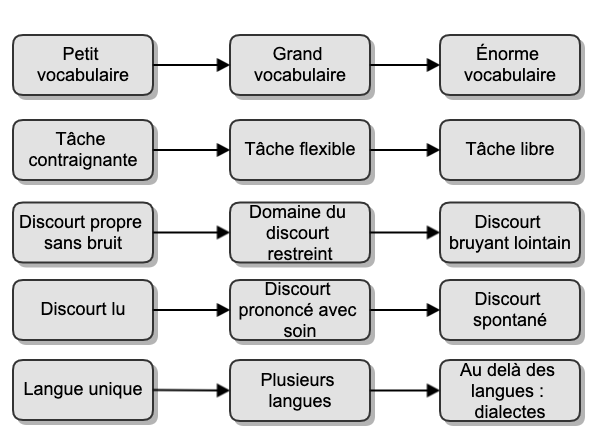
\includegraphics[height=200pt,width=300pt]{images/chap1/evolution_asr.png}
    \caption{Évolution des contraintes lors de la reconnaissance de la parole}
    \label{evolotion}
\end{figure}

\subsection{Utilisation des systèmes de reconnaissance de la parole}
Le fait que la reconnaissance de la parole ait suscité autant d'intérêt ces dernières décennies n'est pas dû au hasard. En effet, ces systèmes sont d'une grande utilité tant pour améliorer la communication entre les humains que la communication entre l'humain et la machine \cite{deeplearningapproach}.

Les systèmes de reconnaissance de la parole peuvent être utilisés, entre autres applications, afin de : 
\begin{itemize}
    \item développer des assistants intelligents basés sur la reconnaissance de la parole qui, de nos jours, sont présents dans beaucoup d'appareils électroniques permettant ainsi à l'utilisateur d'exprimer des requêtes en langage naturel sans avoir à passer par un clavier réduisant ainsi considérablement le temps et les efforts fournis par ce dernier,
    \item faciliter la traduction lors d'une communication orale où les communiquants ne partagent pas la même langue,
     \item gagner en mobilité dans des environnements où une interaction écrite avec nos machines n'est pas possible tel que des travaux manuels ou tout simplement dans sa voiture,
    \item nouveau moyen d'interaction pour les personnes mal voyantes leur permettant ainsi d'interagir avec autrui.
\end{itemize}

\subsection{Architecture d'un système de reconnaissance de la parole basée reconnaissance de phonèmes} \label{Archi1}
Les systèmes basés reconnaissance de phonèmes partagent une architecture commune et ce, indépendamment de la langue traitée. Cette architecture comporte quatre modules principaux qui sont représentés à travers le diagramme suivant \cite{deeplearningapproach} :
\begin{figure}[H]
    \centering
    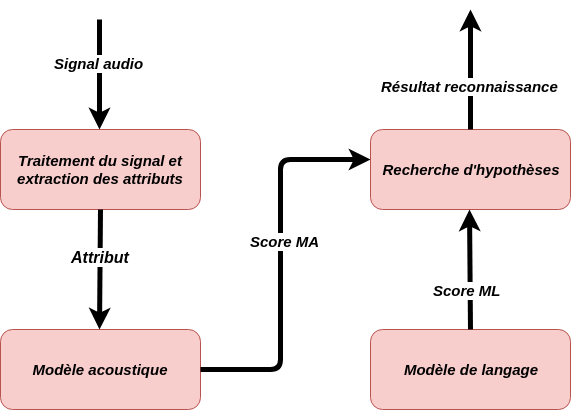
\includegraphics[height=200pt,width=300pt]{images/chap1/architecture_asr.png}
    \caption{Architecture d'un système de reconnaissance de la parole basée reconnaissance de phonèmes}
\end{figure}

Nous présentons dans ce qui suit chaque module de l'architecture :

\subsubsection{Traitement du signal et extraction des attributs}
Traduit de "signal processing and feature extraction", ce module de l'architecture prend un signal audio en entrée, passe par une étape de réduction du bruit suivie de la transformation du signal analogique en fréquences et donne en sortie des vecteurs contenant les caractéristiques de ces fréquences sous forme d'attributs. L'une des méthodes les plus répandues pour l'extraction de ces attributs est l'utilisation du MFCC\footnote{MFCC : Mel Frequency Ceptral Coefficients.} \cite{mfcc} qui prend un enregistrement audio en entrée, y applique un certain nombre de filtres et renvoie en sortie une matrice numérique de caractéristiques qui est un spectrogramme représentant la variation du signal. Nous présentons le MFCC en détail dans le troisième chapitre de ce mémoire.

\subsubsection{Modèle acoustique}
Le modèle acoustique représente la pierre angulaire de cette architecture, il a pour objectif de transformer les informations contenues dans le vecteur de caractéristiques produit par le module précédent (traitement du signal) en unités linguistiques qui seront traitées au niveau du module suivant. \cite{featureextract} présente les approches utilisées pour répondre à ce besoin :
\begin{itemize}
    \item l'approche appelée algorithmes dynamiques de déformation temporelle \cite{terministicapproach} qui a pour but de comparer directement les séquences des données temporelles, tel que des enregistrements audio, en utilisant différentes mesures de distance tel que la distance euclidienne par exemple. Ces approches sont anciennes et très rarement utilisée de nos jours.
    \item l'approche statistique: nous parlons ici de HMM\footnote{Modèles de Markov Cachés, traduit de l'anglais : "Hidden Markov Models"} \cite{hmmtuto} et de GMM\footnote{Modèles de mélange Gaussien, traduit de l'anglais : "Gaussian Mixture Models"} \cite{gmmrobust} mais aussi de modèles d'apprentissage profond ou encore des modèles hybrides HMM-DNN\footnote{Réseaux de Neurones Profonds, traduit de l'anglais "Deep Neural Networks"} \cite{dnnnew}. Ces techniques seront brièvement présentées dans le chapitre 2.	 
\end{itemize}

\subsubsection{Modèle de langage}
Les modèles de langage sont utilisés dans les systèmes de reconnaissance de la parole pour améliorer leur performance. En pratique, ce modèle est utilisé pour rechercher une interprétation de l'entrée du modèle acoustique et prédire une suite de mots correspondant à cette entrée. D'après \cite{languagemodel}, ce modèle peut être basé sur :
\begin{itemize}
    \item une grammaire : Utilisée généralement lorsque la gamme de phrases à reconnaître est restreinte en terme de taille et peut être capturée par une grammaire déterministe. Ce type de modèles est très peu utilisé de nos jours; ou 
    \item un modèle probabiliste, le plus souvent utilisant la notion de N-Grammes \cite{ngramspeech} qui sera détaillée par la suite.\\
\end{itemize}

Le plus grand avantage du modèle de langage est de réduire la perplexité de la reconnaissance en imposant au système de respecter une cohérence dans la suite des mots reconnue par le modèle acoustique et ainsi,  améliorer les performances de la tâche de reconnaissance \cite{langmodelbenefit}.


\subsubsection{Recherche d'hypothèses}
Pour le modèle acoustique et le modèle de langage, un score est généré pour chacun afin d'évaluer le résultat et ce sont ces scores qui sont utilisés dans le module de recherche d'hypothèses.
Ce module compare le score associé au modèle acoustique à celui généré par le modèle de langage afin de décider du résultat final de la reconnaissance. Si le score du modèle de langage est supérieur à celui du modèle acoustique, le système effectue une rectification dans l'ordre d'apparition des mots reconnus  \cite{deeplearningapproach}.
Dans le cas de la reconnaissance de la parole, le score engendré est la performance du modèle qui est représentée par des métriques que nous détaillons dans le chapitre suivant.

La figure \ref{explASRpho} est un exemple de reconnaissance de la parole basée reconnaissance de phonèmes.

\begin{figure}[H]
    \centering
    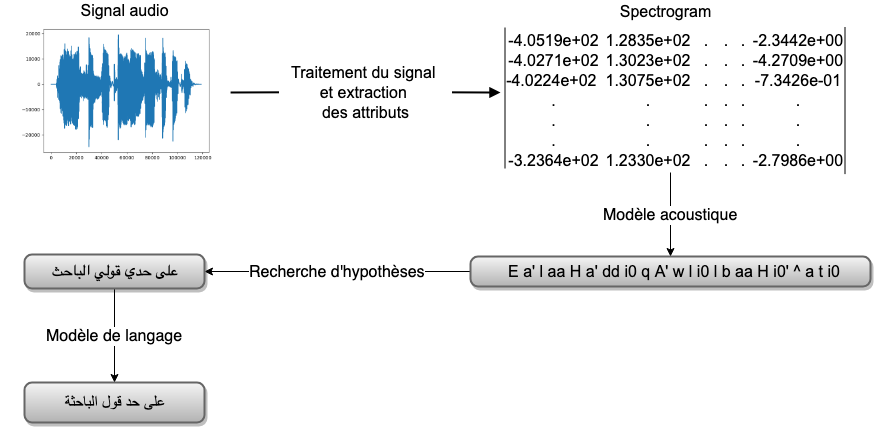
\includegraphics[width=400pt]{images/chap1/Exemple_ASR_Phoneme.png}
    \caption{Exemple de reconnaissance de la parole basée reconnaissance de phonèmes}
    \label{explASRpho}
\end{figure}


\subsection{Architecture End-To-End d'un système de reconnaissance de la parole} \label{Archi2}
L'architecture bout à bout, ou End-To-End en anglais, porte ce nom car contrairement à l'architecture précédente elle consiste en un seul module qui prend en entrée un enregistrement audio et produit la transcription qui y correspond. 
Cette approche pour appréhender les systèmes de reconnaissance de parole a été introduite par \cite{towardse2esr} pour palier aux difficultés rencontrées dans l'approche basée reconnaissance de phonèmes :
\begin{itemize}
    \item complexité de développement
    \item pauvreté des corpus disponibles, et 
    \item barrière de la langue. 
\end{itemize}

Nous commençons par présenter la figure suivante qui illustre les composantes principales de cette architecture : 
\begin{figure}[H]
    \centering
    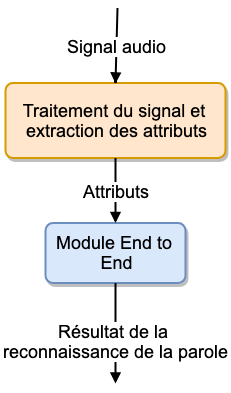
\includegraphics[width=140pt]{images/chap1/E2E_Archi.png}
    \caption{Architecture End-To-End d'un système de reconnaissance de la parole}
\end{figure}

Comme nous le voyons, cette architecture se compose de deux modules principaux.

\subsubsection{Traitement du signal et extraction des attributs}
Ce module a la même fonction que le module portant le même nom dans l'approche basée reconnaissance de phonèmes qui est de générer, à partir d'une enregistrement audio, un spectrogramme sous forme de matrice numérique représentant les variations du signal de l'enregistrement.

\subsubsection{Module End-To-End}
Ce module, que nous considérons pour l'instant comme une boîte noire, est le module qui apprend à générer une transcription à partir d'un spectrogramme jouant ainsi le rôle du modèle acoustique et du modèle de langage. Ce module a donc pour but d'abstraire la difficulté de la tâche de reconnaissance et simplifier le pipeline du développement et ce, en se basant sur des techniques plus récentes d'apprentissage automatique et d'apprentissage profond tel que les réseaux de neurones que nous présentons à travers les deux chapitres suivants.

La figure suivante est un exemple qui a pour but de présenter les étapes de la reconnaissance d'un enregistrement audio pour l'approche End-To-End.

\begin{figure}[H]
    \centering
    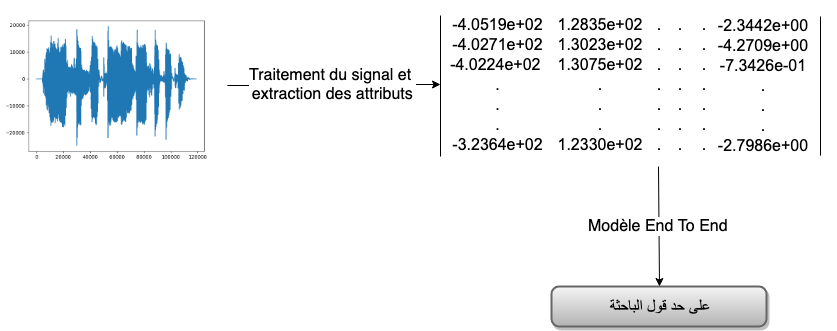
\includegraphics[width=400pt]{images/chap1/Exemple_archi_end2end.png}
    \caption{Exemple de reconnaissance avec l'architecture End-To-End}
    \label{explASRE2E}
\end{figure}


\section{Systèmes de synthèse vocale}
\subsection{Présentation}
Les systèmes de synthèse vocale ou, Text-To-Speech en anglais, sont utilisés pour convertir des mots écrits (dans un document par exemple) en discours audible et doivent êtres capables de lire n'importe quel texte.
Ces systèmes sont largement utilisés de nos jours et il y a de plus en plus d'applications qui fournissant des services de synthèse vocale. L'engouement pour ces systèmes est dû aux possibilités que ceux-ci offrent \cite{ttsuse}, parmis ces possibilités nous citons : 
\begin{itemize}
    \item l'aide aux mal-voyants,
    \item l'aide à l'assimilation des connaissances, 
    \item l'aide à la traduction et à la prononciation, et
    \item les assistants intelligents. \\
\end{itemize}

Comme pour la tâche de reconnaissance de la parole, il existe une approche qui se base sur la synthèse des phonèmes et une approche bout à bout. Nous présentons dans ce qui suit ces deux approches en mettant l'accent sur la complexité de conception d'un système basée synthèse de phonèmes par rapport à un système bout à bout.

\subsection{Architecture d'un système de synthèse vocale basée synthèse de phonèmes}
Les systèmes basés synthèse de phonèmes se basent sur deux parties principales: conversion du texte en phonèmes puis, conversion des caractéristiques linguistiques des phonèmes en discours \cite{textspeechpres}. Nous présentons dans ce qui suit quelques généralités sur cette approche.
Un système de synthèse vocale, indépendamment du texte et de la langue , se compose des modules de base suivants \cite{textspeechmodules} :
\begin{itemize}
    \item \textbf{Conversion de graphème vers phonèmes} : Permet de convertir un texte écrit en phonèmes et ce en utilisant un alphabet phonétique qui est un ensemble de symboles ou de codes utilisés pour indiquer le son d'une lettre (comme Arpabet \cite{arpabet} par exemple).
    \item \textbf{Modèle de segmentation} : il localise les temps de début et fin de chaque phonème et permet d'effectuer un alignement entre les phonèmes ainsi que les lettres présentes présentes dans le catalogue de voix disponible.
    \item \textbf{Modèle de fréquence fondamentale} :  il prédit si un phonème est exprimé et si tel est le cas, il retourne la fréquence du signal correspondante à ce phonème selon la durée de ce dernier.
    \item \textbf{Modèle de synthèse audio} : il combine les sorties des modèles précédents et renvoie en sortie une synthèse vocale du texte désiré. 
\end{itemize}
 
\subsection{Architecture End-To-End d'un système de synthèse vocale}
L'architecture bout à bout \cite{e2espeechsynth} se compose de deux modules principaux comme le montre la figure \ref{E2Esynthese} : 
\begin{figure}[H]
    \centering
    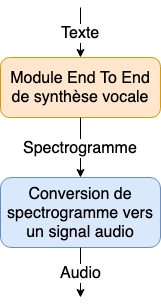
\includegraphics[width=120pt]{images/chap1/Synthese_E2E_Archi.png}
    \caption{Architecture End-To-End d'un système de synthèse vocale}
    \label{E2Esynthese}
\end{figure}

Cette architecture est donc composée des : 

\begin{itemize}
    \item \textbf{Module End-To-End de synthése vocale} : qui prend un texte en entrée et génère à partir de ce texte un spectrogramme. Nous pouvons considérer ce processus comme le processus inverse que celui présenté dans le module séquence à séquence pour les systèmes de reconnaissance de la parole.
    \item \textbf{Conversion de spectrogramme vers signal audio} : ce module permet de convertir un spectrogramme en un signal audio générant ainsi un enregistrement. \\
\end{itemize}

La figure \ref{exempleSyntheseVoc} est un exemple de traduction d'un texte vers un enregistrement sonore à l'aide de l'architecture End-To-End.

\begin{figure}[H]
    \centering
    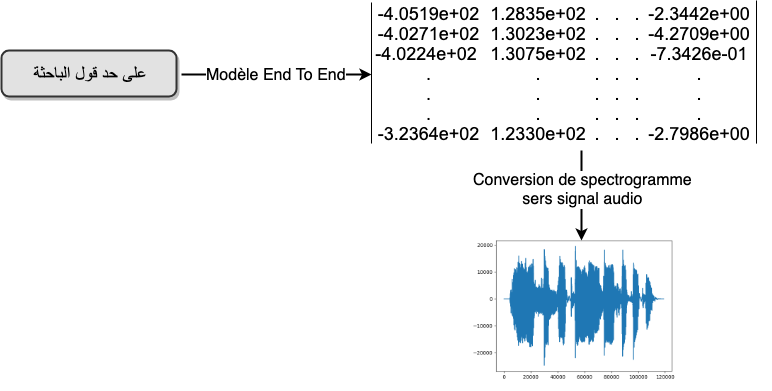
\includegraphics[width=400pt]{images/chap1/Exemple_Synthese_E2E.png}
    \caption{Exemple de synthèse vocale avec l'architecture End-To-End}
    \label{exempleSyntheseVoc}
\end{figure}
\subsection{Quelques applications de synthèse vocale}
Il existe à ce jour plusieurs applications de synthèse vocale \cite{ttsapps}; nous présentons dans ce qui suit les meilleures applications en terme de performance et de simplicité d'utilisation.
\begin{itemize}
    \item \textbf{Amazon Polly} : Alexa n'est pas le seul outil d'intelligence artificielle créé par le géant de la technologie Amazon; il propose également un système de synthèse vocale intelligent appelé Polly \cite{polly} et utilise des techniques avancées d'apprentissage profond. Ce logiciel transforme le texte en discours réaliste et les développeurs peuvent utiliser le logiciel pour créer des produits et des applications embarquant des systèmes de traitement de la parole. Amazon Polly comporte une API permettant d'intégrer facilement les fonctionnalités de synthèse vocale dans des livres électroniques, des articles et d'autres supports. Pour convertir du texte en parole, il suffit de l'envoyer par l'intermédiaire de l'API, qui enverra un flux audio directement à votre application. Amazon Polly est disponible pour plusieurs langues dont l'anglais, le français, le portugais, le japonais et le mandarin. \\
    
    \item \textbf{Voice Reader Home} : basée en Allemagne, Linguatec est une autre société qui crée des applications de synthèse vocale depuis plusieurs années. À présent dans sa 15ème édition, Voice Reader \cite{voicereader} peut convertir rapidement du texte en fichiers audio et peut convertir rapidement des textes tels que des documents Word, des courriels, des EPUB et des PDF pour les écouter sur un PC ou un appareil mobile par la suite. Cette application a l'avantage d'offrir 67 voix différentes et prendre en charge jusqu'à 45 langues telles que l'anglais, l'arabe, le français, l'espagnol, l'italien, le danois et le turc. \\ 
    
    \item \textbf{Capti Voice} : Les applications de synthèse vocale sont également populaires dans le monde de l'éducation, où elles sont notamment utilisées pour améliorer la compréhension. Positionnée comme une solution d'aide à la lecture hors ligne et en ligne, Capti Voice dans sa version 2.0 \cite{captivoice} est utilisée par un grand nombre d'écoles, de collèges, d'entreprises et de professionnels du monde entier. Soutenant plus de 20 langues, dont la langue arabe, l'application peut être utilisée pour améliorer le vocabulaire ainsi que dans le cadre de stratégies de lecture active. Elle peut décrire un éventail de contenus, notamment des livres électroniques, des articles et des pages web. Capti Voice a cependant le désavantage de proposer des licences chères ce qui rend son utilisation très contraignante dans les milieux démunis. \\
    
    \item \textbf{Natural Reader} : c'est une application de synthèse vocale basée sur le cloud et destinée d'avantage à un usage personnel. Natural Reader \cite{naturalreader} permet de convertir des textes écrits tels que des documents Word et PDF, des livres électroniques et des pages Web en des discours continus. Etant basée sur la technologie du cloud, cette application peut accéder au service de synthèse vocale quel que soit le support du moment que l'application est connectée au même service cloud. Natural Reader propose le service de synthèse vocale pour plusieurs langues dont : l'anglais, l'arabe, l'allemand, le français et le mandarin.
\end{itemize}

\subsection{Discussion}
À travers cette présentation, nous notons que le développement d'un système basé synthèse de phonèmes peut s'avérer plus complexe car il nécessite en premier lieu la collecte d'un corpus de données contenant une description des temps de début et de fin de chaque phonème et la collecte d'un tel corpus peut s'avérer délicate comparée à la collecte d'un simple corpus d'enregistrements sonores et transcriptions pour l'approche End-To-End. En plus de cela, l'approche End-To-End présente un développement plus intuitif et plus prometteur grâce à l'avancée des technologies qui y sont utilisées. 

Nous nous contentons de ces généralités en ce qui concerne les architectures des systèmes de synthèse vocale car le corps de notre travail consiste à développer un système de reconnaissance de la parole et son application sur une problématique donnée. Nous introduisons dans ce qui suit les systèmes de questions-réponses, leurs différents types ainsi qu'une présentation de quelques exemples de ces systèmes.

\section{Les systèmes de questions-réponses}
\subsection{Présentation}
Les systèmes de questions-réponses sont des systèmes intelligents. Selon  \newline \cite{QAS}, un système de questions-réponses est un système d'information capable de comprendre des questions et y répondre de manière précise dans un langage naturel humain comme par exemple donner une réponse à la question "Quels sont les meilleurs laboratoires de recherche en intelligence artificielle ?"

Les systèmes de questions-réponses sont généralement classifiés selon le domaine auquel ils appartiennent ainsi que le type de questions.

\subsection{Classification des systèmes de questions-réponses par domaine} \label{QASdomain}
Nous commençons par introduire les deux domaines auxquels peuvent appartenir les systèmes de questions-réponses. D'après \cite{Types_QAS_Survey} ceux-ci peuvent être ouverts ou fermés.
\subsubsection{Domaine ouvert}
Les systèmes de questions-réponses de domaine ouvert sont des systèmes qui ne sont pas limités à un domaine spécifique. En d'autres termes, pour cette classe de systèmes, l'utilisateur a la possibilité d'introduire la question qu'il désire dans le système étant donné que ce type de systèmes recherche généralement les réponses dans une grande collection de documents comme les recherches sur le web à titre d'exemple.

\subsubsection{Domaine fermé}
Les systèmes de questions-réponses appartenant au domaine fermé consistent en un référentiel limité de questions spécifiques à un domaine (le domaine médical à titre d'exemple) et peuvent répondre à un nombre limité de questions. La qualité des réponses dans le domaine fermé est élevée, les réponses sont obtenues à partir de données structurées (telles que des bases de données), des données semi-structurées (par exemple, des textes annotés au format XML) ou des données non structurées (textes libres).
% ici classification des SQR par type de question
\subsection{Classification des systèmes de questions-réponses par types de questions} \label{QASqstType} 
Le type de la question posée par un utilisateur est très important car il permet de déduire, à priori, le type de réponse attendue et ainsi de générer cette dernière d'une manière plus efficace. 
Les différents types de questions posées par les utilisateurs sont classés d'après \cite{qstClassif} en :
\begin{itemize}
    \item questions de type factoïde, 
    \item questions de type liste,
    \item questions de confirmation, et 
    \item questions de causalité.\\
\end{itemize}

Prenons pour exemple la question "Qui était le premier président de l'Algérie?", le domaine de la question posée par l'utilisateur est l'histoire de l'Algérie, la réponse attendue est une entité nommée et plus précisément le nom d'une personne qui est “Ahmed Benbella”. Cette question est de type factoïde.

Dans le tableau \ref{table:qstclass} nous présentons les principaux types de questions.

\FloatBarrier
\begin{center}
    \begin{table}[h]
    \caption{Classification des questions par type  de réponse}
    \label{table:qstclass}
    \begin{tabular}{|c|c|c|}
        \hline
         \thead{Type} & \thead{Réponse attendue} & \thead{Exemple}\\
         \hline
         \makecell[l]{Factoïde} & \makecell[l]{Entité nommée (nom d'une \\ personne nom d'une organisation, \\lieu ou date)} &  \makecell[l]{\textbf{Question} : Quelle est\\la capitale de l'Algérie ?\\ \textbf{Réponse} : Alger.} \\
         \hline
         \makecell[l]{Liste} & \makecell[l]{Une liste d'entités nommées} & \makecell[l]{\textbf{Question} : quels sont les\\ pays les plus propres\\ du monde?\\ \textbf{Réponse} : Suède, Nouvelle\\ Zélande, Australie, \\Canada.}\\
        \hline
        \makecell[l]{Définition}  & \makecell[l]{Information concernant\\ une entité nommée} & \makecell[l]{\textbf{Question} : Qui est \\Thomas Pesquet ?\\\textbf{Réponse} : un spationaute\\français de l'Agence\\spatiale européenne.}\\
        \hline
        \makecell[l]{Confirmation} & \makecell[l]{Les réponses peuvent être de \\ différents types : \\ Oui/Non Arguments, etc.} & \makecell[l]{\textbf{Question} : Est-ce-que\\l'USTHB se situe en Algérie \\ \textbf{Réponse} : Oui.} \\
        \hline
        \makecell[l]{Causale} & \makecell[l]{Des explications sur une entité.} & \makecell[l]{\textbf{Question} : Pourquoi les \\abeilles  produisent du miel? \\ \textbf{Réponse} : Les abeilles \\ fabriquent  du miel pour \\ nourrir les larves  et surtout\\ pour avoir des  réserves de \\nourriture en hiver.}\\
        \hline
    \end{tabular}
    \end{table}
\end{center}
\FloatBarrier

\subsection{Architecture des systèmes de questions-réponses}
L'architecture type d'un système de questions-réponses (voir la figure \ref{ArchiQAS}) se compose de trois modules principaux \cite{thesisasma} : un module d'analyse des questions, un module de traitement des documents et un module d'extraction et validation de la réponse.

\subsubsection{Module d'analyse des questions}
Dans ce module, la question posée par l'utilisateur est analysée afin d'identifier son type, d'en extraire les caractéristiques et la structure de la réponse attendue et de déterminer les contraintes qui pèsent sur la réponse attendue.
\subsubsection{Module de traitement des documents}
Ce module est un composant essentiel du système de questions-réponses. Son rôle est d'extraire les documents et les passages pertinents pour la question à partir d'une collection de données (Web ou autre) pour effectuer ensuite un processus de classement qui permettra d'améliorer la pertinence des passages candidats qui correspondent le mieux à la question de l'utilisateur.
\subsubsection{Module d'extraction et validation de la réponse}  
Dans les systèmes de questions-réponses, ce module peut être conçu pour extraire la réponse à partir d'un ou plusieurs passages. Ce module ne renvoie la réponse que si les passages candidats fournis par le module de traitement des documents sont pertinents et contiennent réellement la réponse. Certains systèmes intègrent également la validation des réponses dans ce module. 
\begin{figure}[H]
    \centering
    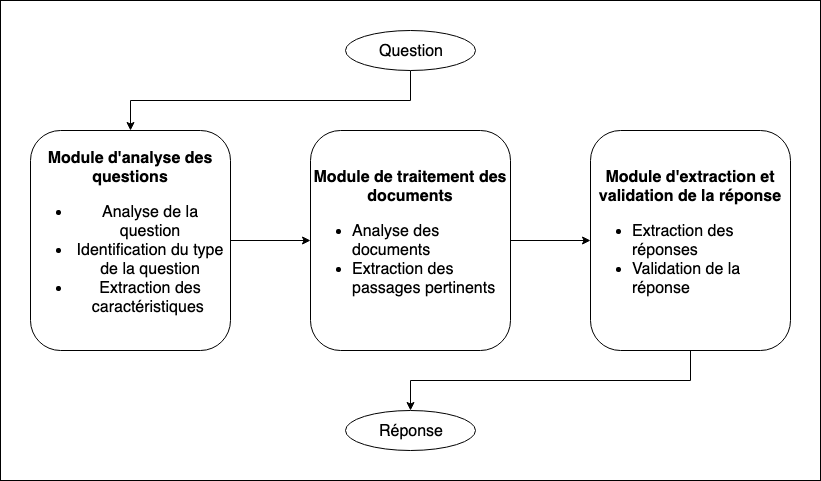
\includegraphics[height=200pt,width=325pt]{images/chap1/QAS_archi.png}
    \caption{Architecture générique d'un système de questions-réponses}
    \label{ArchiQAS}
\end{figure}


\subsection{Quelques systèmes de questions-réponses}
Les systèmes de questions-réponses pour la langue arabe ne sont pas aussi nombreux que pour l'anglais par exemple, ce qui peut s'expliquer par le nombre limité de corpus de qualité existants.

Dans ce qui suit, nous présentons quelques exemples de systèmes de questions-réponses pour la langue anglaise et la langue arabe.


\subsubsection{Start}
START est un des systèmes de questions-réponses les plus connus pour la langue anglaise. Développé par Boris Katz et ses collaborateurs du groupe InfoLab du laboratoire d'informatique et d'intelligence artificielle du MIT, START est en ligne depuis 1993 \cite{StartPaper}. Actuellement, ce système peut répondre à des millions de questions en anglais en langage naturel. Les réponses sont en format texte ou multimédia qui sont tirés d'un ensemble de ressources d'informations hébergées localement ou accessibles à distance via Internet.

% START vise une grande précision dans la réponse à ses questions et, en grande partie, sa capacité à répondre aux questions se fait grâce à l'utilisation des annotations en langage naturel en tant que mécanisme d'ajustement des questions aux réponses des candidats. 

% Lorsque de nouvelles ressources d'information sont incorporées pour l'utilisation de START, les annotations en langage naturel sont souvent composées manuellement - généralement à un niveau abstrait - puis associées à divers composants d'information. Bien que l'effort START ait également exploré diverses techniques pour la génération automatique d'annotations, le présent document porte sur l'utilisation des annotations composées manuellement dans START et ses systèmes affiliés, ainsi que sur les avantages qui en découlent.

% \subsection{Travaux sur la langue arabe}
% L'arabe est la 6ème langue naturelle la plus répandue au monde avec plus de 350 millions de locuteurs natifs. Les systèmes de questions-réponses en arabe gagnent en importance en raison de la quantité croissante du contenu en arabe et de la demande croissante d'informations que les techniques habituelles de recherche d'information ne peuvent satisfaire.
% Malgré cela, ces systèmes rencontrent des difficultés en terme de ressources. Comparé à d'autres langues, les corpus utilisés sont peu volumineux et manquent en diversité du contenu. Dans ce qui suit nous présentons les systèmes que nous jugeons être les plus intéressants en la matière.

\subsubsection{DefArabicQA}
DefArabicQA \cite{ArabicQA}  est un système de questions-réponses de définition, en d'autres termes ce système traite les questions du type \setcode{utf8}\<ما هو ؟> ou \setcode{utf8}\<ما هي ؟> . Il identifie les définitions candidates en utilisant un ensemble de modèles lexicaux \footnote{Un modèle lexical est une séquence de chaînes de caractères (par exemple, des mots, des lettres et des signes de ponctuation) qui fournissent un contexte pour identifier les réponses exactes \cite{ArabicQA}.}, filtre ces définitions candidates en utilisant des règles heuristiques qui se déduisent de l'observation d'un ensemble de définitions candidates annotées\footnote{Un ensemble de définitions candidates divisées en définitions de candidats incorrectes et correctes} et les hiérarchise en utilisant une approche statistique. Le type de réponse attendu est déduit par la suite du pronom interrogatif de la question.
% Dans \cite{ArabicQA}, Trigui1 et al. ont effectué deux expériences d'évaluation sur 50 questions de définition. 
% \begin{center}
%     \begin{table}[H]
%         \centering
%         \begin{tabular}{|c|c|c|}
%             \hline
%             \thead{Expérience} & \thead{ressource Web} & \thead{MRR}\\
%             \hline
%             \makecell{1} & \makecell{Google} & \makecell{0,70}  \\
%             \hline
%             \makecell{2} & \makecell{Google couplé \\ à Wikipédia} & \makecell{0,81}  \\
%             \hline
%         \end{tabular}
%         \caption{Expériences d'évaluation de DefArabicQA}
%         \label{tab:my_label}
%     \end{table}
% \end{center}

\subsubsection{Al-Bayan}
Al-Bayan \cite{Albayan} est un système de questions-réponses spécifique au Coran. Il prend une question en arabe en entrée et récupère des versets  accompagnés de leur \textit{tafsir} (interprétation des versets) sémantiquement pertinents en tant que passages candidats.

La spécificité de ce système réside dans le fait qu'il automatise le processus de sélection des réponses. Les réponses candidates sont ensuite classées en :
\begin{itemize}
    \item Réponses qui répondent directement à la question.
    \item Réponses qui peuvent être utiles.
    \item Réponses qui ne sont pas pertinentes.
\end{itemize}


\section{Conclusion}
Au vu de l'importance des systèmes de reconnaissance de la parole, l'étude de ces derniers et leur implémentation pour la langue arabe dans des applications telles que les systèmes de questions-réponses est devenu un besoin pour le monde arabe en particulier et pour les utilisateurs de l'arabe de manière générale. Au cours de ce chapitre, nous avons abordé les aspects de bases des systèmes de reconnaissance de la parole, systèmes de synthèse vocale ainsi que des systèmes de questions-réponses comme cas d'application pour la reconnaissance de la parole.

Dans le chapitre suivant, nous introduisons les différentes approches utilisées pour le développement d'un système de reconnaissance de la parole pour ensuite présenter les travaux faisant état de l'art tant pour la langue arabe que pour les autres langues afin de nous guider à concevoir notre propre système.

    

\chapter{Travaux sur les systèmes de reconnaissance de la parole}
\section{Introduction}
L'utilisation des systèmes de reconnaissance de la parole permet d'accéder à l'information de manière rapide et intuitive. Aujourd'hui, beaucoup de nos appareils électroniques ont une exploitation plus naturelle car ils embarquent des fonctionnalités de reconnaissance de la parole. Cependant, nous remarquons que ces systèmes traitent rarement la langue arabe de manière efficace.

Dans ce chapitre nous présentons l'état de l'art pour les systèmes de reconnaissance de la parole et notamment pour la langue arabe. Mais avant cela, nous définissons les différentes techniques et approches utilisées pour la conception des systèmes End-To-End et des systèmes basés reconnaissance de phonèmes pour la reconnaissance de la parole.

\section{Techniques utilisées pour l'approche End-To-End}
\cite{ml} définit l'apprentissage automatique comme étant un programme informatique qui apprend d'une expérience \textit{E} à l'égard de certaines classes de tâches \textit{T} et de la mesure de performance \textit{P}. Si sa performance aux tâches en \textit{T}, la performance mesurée par \textit{P}, s'améliore avec l'expérience \textit{E}.\\ En d'autres termes, l'apprentissage automatique est une technique d'intelligence artificielle basée sur différentes notions mathématiques et plus particulièrement statistiques. Elle permet aux ordinateurs d'apprendre à partir des données et résoudre des problèmes ou effectuer des tâches complexes sans être explicitement programmés à cet effet \cite{Goodfellow-et-al-2016}.

L'apprentissage automatique se présente sous plusieurs types et ce en fonction du problème et du jeu de données à disposition. Ces types sont l'apprentissage supervisé, l'apprentissage non supervisé et l'apprentissage par renforcement \cite{typesml}. Pour la conception de notre système, nous nous intéressons au paradigme d'apprentissage supervisé.

L'apprentissage est dit supervisé lorsque le système apprend à classer des données à partir d'un algorithme d'entraînement\footnote{Nous utilisons pour la suite de ce document l'expression : Algorithme d'apprentissage}, traduit de "training" en anglais, ainsi que des exemples de données connus \cite{supervised}. Ce type d'apprentissage se divise en deux parties :
\begin{itemize}
    \item la première correspond à générer un modèle ayant la capacité de prédire la classe d'un ensemble de données qu'il rencontre pour la première fois. La génération de ce modèle se fait grâce à un algorithme d'apprentissage ainsi qu'à des données étiquetées (labelisées), et
    \item la deuxième consiste à prédire l'étiquette d'une nouvelle donnée dont nous ignorons le label à partir du modèle préalablement généré. \\
\end{itemize}

Comme mentionné dans le chapitre précédent, l'architecture End-To-End se base sur différents types de réseaux de neurones pour permettre de prédire la transcription associée à une entrée audio. Ce choix d'algorithme d'apprentissage, en plus des avantages classiques des réseaux de neurones, se justifie par :\\
\begin{itemize}
    \item la capacité d'apprendre et de modéliser des relations complexes et non-linéaires ce qui est le cas lorsqu'il s'agit d'associer du texte à de la parole, et
    \item contrairement à beaucoup d'autres techniques, certains réseaux de neurones tels que les réseaux récurrents n'imposent pas de restriction en terme de taille des données aux variables d'entrée. Dans notre cas, les données sont des séries chronologiques, traduit de Time Series en anglais, et se présentent sous forme de séquences de taille variable. Étant donné leur capacité à apprendre des relations cachées entre les données, les réseaux de neurones sont la solution de prédilection à notre problématique. \\
\end{itemize}

Nous présentons dans ce qui suit les différents types de réseaux de neurones ainsi que ce qu'ils peuvent apporter à notre tâche.

\subsection{Réseaux de neurones artificiels}
Les réseaux de neurones artificiels, ou Artificial Neural Networks (ANN) en anglais, sont des réseaux fortement connectés de processeurs élémentaires fonctionnant en parallèle. Chaque processeur élémentaire calcule une sortie unique sur la base des informations qu'il reçoit \cite{neuralnetsbook}. Ces réseaux artificiels sont inspirés de l'interconnexion des neurones chez les êtres vivants et sont composés d'une succession de couches où chacune prend ses entrées depuis les sorties de la couche précédente. 
De base, tout réseau de neurones est composé d'une couche d'entrée, une ou plusieurs couches cachées et une couche de sortie comme le montre la figure suivante \cite{neuralnetsbook} : 

\begin{figure}[H]
    \centering
    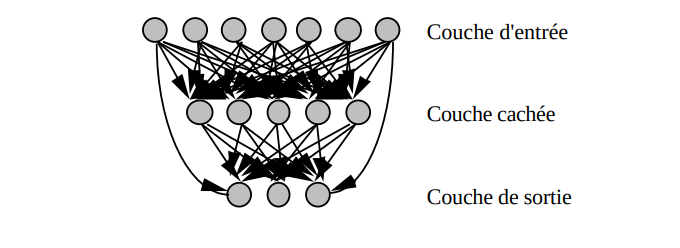
\includegraphics[height=150pt,width=325pt]{images/chap2/neural_net.png}
    \caption{Couches d'un réseau de neurones}
\end{figure}

Il existe plusieurs catégories de réseaux de neurones artificiels, \cite{neuralnetsbook} les classifie en : \\
\begin{itemize}
    \item \textbf{Réseaux multicouche} : Les connexions se font entre les neurones des couches en aval, et chaque neurone d'une couche est connecté à tous les neurones de la couche suivante et celle-ci seulement.
    \item\textbf{Réseaux à connexions locales} : Chaque neurone entretient des relations avec un nombre réduit et localisé de neurones de la couche avale.
    \item \textbf{Réseaux à connexion complète} : Structure d'interconnexion la plus générale où chaque neurone est connecté à tous les neurones du réseau.
\end{itemize}

\subsection{Réseaux de neurones profonds}
Les réseaux de neurones profonds, traduits de l'anglais Deep Neural Networks (DNN), sont des réseaux qui se composent de plusieurs couches cachées où chaque type de couche présente des avantages pour des cas d'utilisation spécifiques. Cependant, quelque soit l'architecture interne de ces réseaux, ces derniers partagent la même intuition des réseaux de neurones qui consiste à introduire des données et entraîner le modèle à interpréter ces dernières et à prédire un label qui, dans notre cas, est la transcription d'une entrée audio.

Dans le cas de l'architecture End-To-End du système de reconnaissance de la parole, nous nous intéressons aux réseaux de neurones récurrents et réseaux à convolutions.

\subsubsection{Réseaux de neurones récurrents}
Les réseaux de neurones récurrents, ou Recurrent Neural Networds (RNN) en anglais, font partie d'un groupe plus large d'algorithmes appelés modèles de séquence. Les modèles de séquence ont fait des pas de géant dans les domaines qui traitent des données séquentielles comme la reconnaissance de la parole, la génération de musique, l'analyse des séquences ADN ou encore la traduction automatique \cite{rnntowardsdata}. Les réseaux de neurones récurrents sont idéals pour appréhender ce genre de problèmes car contrairement aux réseaux de neurones classiques (ou encore les réseaux à convolutions que nous présentons dans ce qui suit), ces réseaux sont conçus pour prendre une série d'entrées sans déterminer leur taille au préalable. \\
Le point fort des RNNs reste néanmoins leur capacité à mémoriser les suites de séquences de données ce qui s'avère essentiel pour la reconnaissance de la parole \cite{rnnintro}. En effet ces réseaux se souviennent des séquences de données passées et la décision à prendre (classification par exemple) est influencée par ce qui a été appris du passé et ce grâce à une composante de ce réseau qui est le vecteur d'états cachés ou Hidden States Vector en anglais. 

La figure suivante \cite{rnnschema} détaille le flux de l'information dans ce réseau.
\begin{figure}[H]
    \centering
    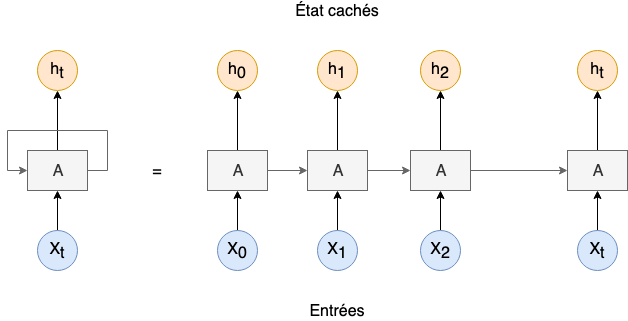
\includegraphics[height=175pt,width=300pt]{images/chap2/RNN.png}
    \caption{Réseau de neurones récurrent}
\end{figure}

Nous remarquons donc qu'à chaque timestep \footnote{Timestep : Pas de temps ou découpe temporelle d'une donnée}, le RNN génère un output ainsi qu'un vecteur d'états cachés qui fera office d'input pour le prochain timestep. \\
Le vecteur d'états cachés est une représentation abstraire du séquencement des données et c'est cette information qui permet au réseau de prendre en compte les informations précédentes à l'instant \textbf{t}. Il est cependant important de noter que les RNNs souffrent, lorsque la taille des séquences est suffisamment grande, du problème du \textit{Vanishing Gradient} qui arrive lorsque les poids du modèle ne sont plus mis à jour et que le gradient avoisine le zero. Il existe néanmoins d'autres réseaux tel que les LSTMs\footnote{Long Short-Term Memory : type de réseau récurrent que nous détaillons dans le chapitre suivant.} basés sur le principe des réseaux de neurones récurrents et qui évitent le \textit{Vanishing Gradient} \cite{vanishinggradient}.  

\subsubsection{Réseaux de neurones à convolutions}
Les réseaux de neurones à convolutions, ou Convolutional Neural Networks (CNN) en anglais, ont été introduits par \cite{cnnhist} et sont analogues aux réseaux de neurones classiques car ils sont composés de neurones qui s'auto-optimisent par l'apprentissage \cite{cnnintro}. L'une des plus grandes limitations des réseaux de neurones traditionnels est qu'ils ne donnent pas de bon résultats avec des données multi-dimensionnelles au vu de  la complexité de calcul et c'est là où réside la grande différence entres les réseaux à convolutions et les ANNs. Un CNN est capable de capturer avec succès les dépendances spatiales et temporelles des données grâce à l'application de filtres appropriés. L'architecture s'ajuste mieux aux données spatiales ou encore séquentielles en raison de la réduction du nombre de paramètres impliqués comme c'est le cas des images, des vidéos ou encore du son comme dans notre cas. Dans un CNN, deux opérations sont appliquées : 
\begin{itemize}
    \item \textbf{Convolution :} Consiste à appliquer un masque de convolution de taille \textbf{(M $\times$ M)} sur l'image en spécifiant un nombre de filtres afin d'extraire les informations pertinentes sous forme d'un ensemble de matrices (ou de filtres) de taille \textbf{(N-M+1 $\times$ N-M+1)}.    
    \item \textbf{Pooling :} Il existe deux variantes pour cette opération: Pooling Maximum et Pooling Moyen. Cette opération consiste à appliquer un masque de taille \textbf{(M $\times$ M)} à la matrice et ne garder que le maximum ou la moyenne de ce masque selon que nous appliquons un Pooling Maximum ou moyen et générer un ensemble de matrices de taille \textbf{(N/M $\times$ N/M)}.\\
\end{itemize}

La figure suivante illustre le fonctionnement d'un réseaux de neurones à convolution à travers un exemple numérique pour une image en 2D.
\begin{figure}[H]
    \centering
    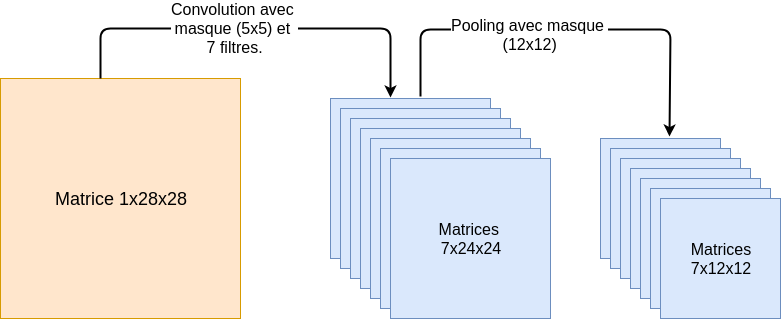
\includegraphics[height=150pt,width=300pt]{images/chap2/CNN.png}
    \caption{Réseau de neurones à convolution}
\end{figure}

Dans le cadre de ce projet, nous traitons des enregistrements audio qui sont des données de type séries temporelles, ces données sont sous forme de vecteurs d'attributs nous utilisons donc des réseaux de neurones à convolution en 1D \cite{cnn1d}. La logique de fonctionnement de ces réseaux est la même à la différence que les masques de convolution et de pooling sont des vecteurs en une dimension au lieu de matrices en deux dimensions pour le cas des images.

\section{Approches utilisées pour les systèmes de reconnaissance basés reconnaissance de phonèmes}
\subsection{Modèle acoustique}  
\subsubsection{Modèles de Markov Cachés}
Traduit de Hidden Markov Models (HMM), les Modèles de Markov Cachés est une approche probabiliste permettant de représenter des distributions de probabilités à partir d'une chaîne d'observations. Par définition, un modèle de Markov caché est un processus doublement stochastique avec un processus sous-jacent non observable (processus caché) mais pouvant uniquement être observé au moyen d'un autre ensemble de processus stochastiques produit à partir de la séquence d'événements observée \cite{hmmdef}. Ces modèles sont basés sur deux propriétés. Premièrement, l'observation à l'instant \textit{t} a été générée par un processus dont l'état \textit{S} est caché à l'observateur. Deuxièmement, nous supposons que l'état du processus caché satisfait la propriété de Markov qui dit qu'étant donné la valeur de l'état \textit{$S_{t-1}$}, l'état actuel \textit{$S_{t}$} est indépendant de tous les états antérieurs à \textit{t - 1}. En d'autres termes, à un moment donné, l'état résume tout ce que nous devons savoir sur l'historique du processus afin de prédire son avenir \cite{hmmdef2}.

Afin d'illustrer ce que nous venons d'expliquer nous prenons l'exemple suivant \cite{hmmexample} : 
\begin{figure}[H]
    \centering
    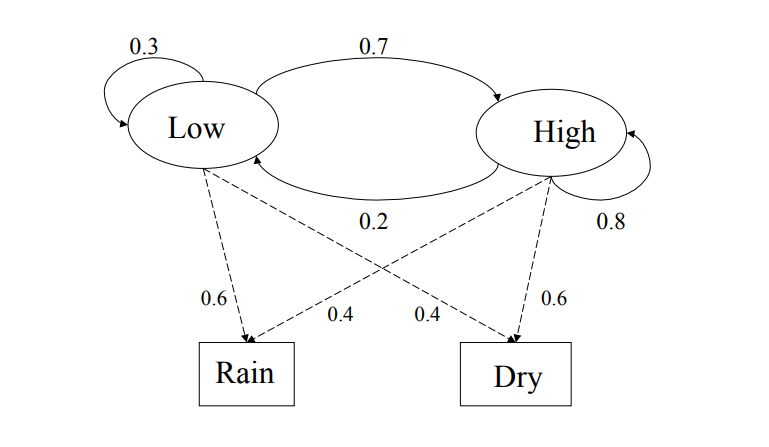
\includegraphics[width=350pt]{images/chap2/hmm_example.png}
    \caption{Exemple Modèle de Markov Caché}
\end{figure}

\begin{itemize}
    \item High et Low sont les états et Rain et Dry sont les observations.
    \item Les probabilités de transition sont : P(Low|Low)=0.3 , P(High|‘Low)=0.7 ...
    \item Les probabilités d'obvservation sont : P(‘Rain'|‘Low')=0.6, P('Dry'|'Low')=0.4 ...
    \item Les probabilités initiales sont : P('Low')=0.4, P('High')=0.6.
\end{itemize}

Une chaîne de Markov Caché nous permet de calculer la probabilité d'une séquence d'observations. Dans le cas de la reconnaissance de la parole nous utilisons cette propriété pour calculer la probabilité de d'avoir une suite de phonèmes sachant un ensemble d'observations (le spectrogramme) et un ensemble d'états (les phonèmes).
Afin de tirer profit des HMMs pour la conception du modèle acoustique, nous avons besoin du vecteur de distributions de probabilités. Pour cela nous pouvons utiliser des Modèles de Mélange Gaussien.

\subsubsection{Modèles de Mélange Gaussien}
Traduit de "Gaussian Mixture Models (GMM)", les Modèles de Mélange Gaussien consistent en une fonction de densité de probabilité paramétrique représentée par la somme pondérée de valeurs Gaussiennes.

Les GMMs sont couramment utilisés comme modèle paramétrique de la distribution de probabilité de mesures ou de caractéristiques continues dans un système biométrique, telles que les caractéristiques spectrales liées au tract vocal dans un système de reconnaissance de la parole \cite{gmmdef}.

Les GMMs permettent de calculer la vraisemblance de variables aléatoires continues offrent ainsi la possibilité de modéliser les distributions de probabilités sur des vecteurs d'entités en entrée associés à chaque état d'un HMM.
Malgré tous leurs avantages, les GMMs présentent un grave inconvénient: ils sont statistiquement inefficaces pour modéliser des données situées sur ou à proximité d'une variété non linéaire dans l'espace de données \cite{dlacoustic}. Dans le cas des systèmes de reconnaissance de la  parole, le discours est produit en modulant un nombre relativement réduit de paramètres, ce qui implique que sa véritable structure sous-jacente est beaucoup plus petite que ce qui apparaît immédiatement dans un vecteur contenant des centaines de caractéristiques.


\subsection{Modèle de langage}
Dans un système de reconnaissance de la parole, un modèle de langage peut être créée à partir du principe de N-gramme. Un N-gramme est une suite de \textit{N} caractères, mots ou même phonèmes qu'on peut retrouver dans une chaîne de caractères ou plus généralement dans un texte \cite{speechlangprocessing}. À titre d'exemple, la phrase : "ce projet est passionnant" contient :
\begin{itemize}
    \item Quatre 1-grammes (ou Uni-grammes) qui sont des chaînes de caractère de longueur de un mot à savoir : "ce", "projet", "est" et "passionnant".
    \item Trois 2-grammes (ou Bi-grammes) qui sont : "ce projet", "projet est" et "est passionnant".
    \item Deux 3-grammes (ou Tri-grammes) qui sont : "ce projet est" et "projet est passionnant".
    \item Un 4-grammes qui est la phrase entière.\\
\end{itemize}

Le choix du N-gramme à utiliser dépend de la structure de la langue que nous voulons traiter (la langue arabe dans notre cas). Utiliser un N-gramme avec un \textit{N} trop petit risquerait de ne pas permettre au modèle de langage de détecter les incohérence dans les suites de phonèmes reconnues par le modèle acoustique. Par ailleurs, si la suite de mots est trop longue nous pouvons nous retrouver dans un cas de sur-apprentissage\footnote{Désigne le fait qu'un modèle s'adapte bien aux données d'apprentissage et présente de très bons résultats mais, présente des résultats bien inférieurs une fois face à des données qu'il n'a jamais croisé \cite{underoverfitting}.} et donc de mémoriser les phonèmes associés à une entrée audio rencontrée pendant la phase d'entraînement mais donner de mauvais résultats pour de nouvelles entrées audio non rencontrées.

\section{Mesures de performances}

Il existe plusieurs mesures possibles pour évaluer la performance d'un système de reconnaissance de la parole.
Nous présentons les quatre métriques que nous utiliserons pour la suite de ce mémoire afin d'évaluer différents systèmes et architectures.

\subsection{Taux d'erreur des mots}
Le taux d'erreur de mots, traduit de Word Error Rate (WER) en anglais, est utilisé pour la reconnaissance continue des mots et où la taille d'une séquence n'est pas prédéfinie. Cette mesure est calculée à partir de la formule suivante \cite{werformula} : \\
        \begin{equation}
            WER = \frac{S + D + I}{N}
        \end{equation}
        où :\\
        S : nombre de mots qui ont été substitués lors de la reconnaissance.\\
        D : nombre de mots qui n'ont pas été écoutés ou ont plutôt été supprimés.\\
        I : nombre de mots qui ont été rajoutés sans qu'ils soient présents dans la parole.\\
        N : nombre total de mots de l'entrée.
        
\subsection{Taux d'erreur de caractères}
Le taux d'erreur de caractères, traduit de Character Error Rate CER en anglais, est une mesure similaire à la métrique WER. Celle ci est généralement utilisée pour mesurer la performance de l'architecture End-To-End où le résultat de la reconnaissance peut être une suite de caractères. Cette mesure est calculée à partir de la formule suivante : \\
        \begin{equation}
            CER = \frac{S + D + I}{N}
        \end{equation}
        où :\\
        S : nombre de caractères qui ont été substitués lors de la reconnaissance.\\
        D : nombre de caractères qui n'ont pas été écoutés ou ont plutôt été supprimés.\\
        I : nombre de mots qui ont été rajoutés sans qu'ils soient présents dans la parole.\\
        N : nombre total de caractères de l'entrée.

\subsection{Exactitude des mots}
L'exactitude des mots ou, Word Accuracy en anglais, est une mesure que nous utilisons lors de  l'entraînement de notre modèle afin de visualiser la performance de ce dernier et ainsi modifier les paramètres utilisés en fonction du besoin. Cette mesure est calculée à partir de la formule suivante :\\ 
    \begin{equation}
    WAcc = 1 - WER = \frac{N - S - D - I}{N} = \frac{H - I}{N}
    \end{equation}
    où : \\
        S : nombre de mots qui ont été substitués lors de la reconnaissance.\\
        D : nombre de mots qui n'ont pas été écoutés ou ont plutôt été supprimés.\\
        I : nombre de mots qui ont été rajoutés sans qu'ils soient présents dans la parole.\\
        N : nombre total de mots de l'entrée.\\    
        H : nombre de mots correctement reconnus.

\subsection{Exactitude des caractères}
L'exactitude des caractères ou, Character Accuracy en anglais, est une mesure que nous utilisons lors de  l'entraînement de notre modèle afin de visualiser la performance de ce dernier et ainsi modifier les paramètres utilisés en fonction du besoin. Cette mesure est calculée à partir de la formule suivante :\\ 
    \begin{equation}
    CAcc = 1 - CER = \frac{N - S - D - I}{N} = \frac{H - I}{N}
    \end{equation}
    où : \\
        S : nombre de caractères qui ont été substitués lors de la reconnaissance.\\
        D : nombre de caractères qui n'ont pas été écoutés ou ont plutôt été supprimés.\\
        I : nombre de caractères qui ont été rajoutés sans qu'ils soient présents dans la parole.\\
        N : nombre total de caractères de l'entrée.\\    
        H : nombre de caractères correctement reconnus.


% \subsection{Mesure pour les systèmes de questions-réponses}
% La métrique que nous utilisons pour évaluer la performance d'un système de questions-réponses est le Rang Réciproque Moyen.\\
% Traduit de "Mean Reciprocal Rank (MRR)", le Rang Réciproque Moyenf  est une mesure statistique permettant d'évaluer tout processus produisant une liste de réponses possibles à un échantillon de questions. Ces réponses sont classées par probabilité d'exactitude\cite{MRR}.\\
% Le MRR est calculé comme suit: \\ 
% \begin{center}
%   MRR = $\sum_{i=1}^{n}\frac{1}{R_{i}}$ 
% \end{center}
% où :
% \begin{itemize}
%     \item n : le nombre de questions du test
%     \item $R_{i}$ : le rang de la première réponse correcte pour la i\_eme question du test.
% \end{itemize}

 
%Si aucune des cinq chaînes de réponse ne contient de réponse, la question se voit attribuée un score de zéro. 
%La valeur de MRR pour l'expérience est calculée en prenant la moyenne des scores pour toutes les questions.
% YAS : je m'explique la 2 eme phrase j'ai décidé de la commenter psq ça a été le cas que dans un seul travail en gros un seul article que j ai lu donc ce n'est pas correcte de le mettre dans une définition et c'est la même chose pour la 1 ere remarque%

%\subsubsection{Rappel et précision}
%Nous commençons par présenter la matrice de confusion qui est une table NxN qui résume la corrélation entre les étiquettes et les classifications du modèle. L'axe des x est% 
%la classe prédite par le modèle, et l'axe des y représente la classe réelle. N correspond au nombre de classes%.
%\begin{center}
%    \begin{table}[H]
%        \centering
%        \begin{tabular}{|c|p{3cm}|p{3cm}|}
%            \hlin%e
%            \backslashbox{Classe réelle}{Classe prédite} & Oui & Non \\
%            \hlin%e
%            Oui & Vrais positifs (VP) & Faux négatifs (FN) \\
%            \hlin%e
%            Non & Faux positifs (FP) & Vrais négatifs (VN)\\ 
%            \hline
       % \end{tabular}
%        \caption{Matrice de confusion}
%        \label{tab:my_label}
%    \end{table}
%\end{center}
%\FloatBarrier
%Le rappel est une mesure statistique qui donne la proportion d'éléments bien classés par rapport au nombre d'éléments à prédire \cite{typesml}. 
%ou ça : Le rappel est une mesure statistique qui répond à la question suivante : Parmi toutes les étiquettes positives possibles, combien d'entre elles le modèle a-t-il correctement identifié ?, i think the other one is good % 
%\begin{center}
 %  Rappel = $\frac{VP}{VP + FN \footnote{Exemple dans lequel le modèle a prédit à tort la classe négative}}$ 
%\end{center}
%La précision est également une mesure statistique qui correspond à la proportion d'éléments bien classé pour une classe donnée \cite{typesml}.
% La précision correspond à la fréquence à laquelle le modèle prédit correctement la classe positive.

%\begin{center}
 %  Précision = $\frac{VP}{VP+ FP\footnote{Exemple dans lequel le modèle a prédit à tort la classe positive}}$ 
%\end{center}

%\subsubsection{F-mesure}
%La F-mesure est une mesure populaire qui combine la précision et le rappel en utilisant la formule suivante: 
%\begin{center}
%   F-mesure = $\frac{2 \times Précision \times Rappel}{Précision + Rappel}$ 
%\end{center}

\section{Systèmes de reconnaissance de la parole les plus performants}
Nous effectuons une comparaison entre les deux types de système de reconnaissance de la parole en commençant par présenter les systèmes basés reconnaissance de phonèmes.

\subsection{Systèmes basés reconnaissance de phonèmes}
Nous présentons dans cette partie les systèmes de reconnaissance de la parole qui sont basés reconnaissance de phonèmes les plus performants \cite{asrreview}.

\subsubsection{Dragon Mobile SDK}
Dragon Mobile SDK est un système closed source \footnote{Un logiciel Closed Source est un logiciel dont le code source est gardé en toute sécurité et crypté. Cela signifie que l'utilisateur ne peut pas copier, modifier ou supprimer des parties du code sans conséquence. Cela peut aller de l'annulation de la garantie à des répercussions juridiques} Développé par Nuance Communication \cite{dragonsdk}, leader mondial du développement de systèmes de reconnaissance de la parole. Ce système client serveur est apprécié pour sa documentation riche ainsi que le nombre important de frameworks\footnote{désigne un ensemble cohérent de composants logiciels structurels, qui sert à créer les fondations ainsi que les grandes lignes de tout ou d'une partie d'un logiciel (architecture)} qu'il propose.
Ce système utilise la plate-forme Speech Kit, également développée par Nuance communication, permettant une simple intégration des systèmes de reconnaissance et synthèse vocale. Cette plateforme fournit ces services à travers un accès asynchrone à des serveurs minimisant ainsi les coûts d'exécution en terme de temps et de ressources matérielles.
Dragon Mobile SDK\footnote{Software Development Kit (SDK): est un ensemble d'outils logiciels destinés aux développeurs et facilitant le développement d'un logiciel sur une plateforme donnée} \cite{dragonsdk} est l'un des systèmes les plus performants pour la langue anglaise avec un taux d'erreur avoisinant les 1\% \cite{asrreview} mais a le gros désavantage de ne permettre qu'un nombre limité de requêtes par jour dans sa version gratuite.


\subsubsection{Google Speech Recognition}
Produit du géant Google, Google Speech Recognition est un système closed source présent sur tout type de support sous système Android ou tout simplement intégrant l'API \cite{googleapi}. Cette dernière a un taux d'erreur de mots (WER) d'environ 2\% \cite{googleapiwer}, un temps de réponse moyen très court et a l'avantage de ne pas limiter le nombre de requêtes par jour, ce qui en fait l'un des systèmes de reconnaissance de la parole les plus utilisés \cite{asrreview}.

\subsubsection{Microsoft Speech API}
Microsoft Speech API est le système de reconnaissance de la parole closed source développé par Microsoft \cite{microsoftapi} et offrant une interface appelée Microsoft Speech Application Programming Interface (SAPI) qui, combiné au Microsoft Speech SDK, offre des services de commande vocale. Cette API comprend un ensemble de méthodes et de données efficaces et bien intégrées au .NET Framework, fournissant ainsi une plate-forme de développement accessible et facile d'intégration d'où l'avantage de ce système. Bien que la Microsoft Speech API soit semblable à la Google Speech Recognition API en terme d'accessibilité et de temps de réponse, celle ci présente néanmoins un taux d'erreur de 5.1\% \cite{msapiwer} supérieur à celui fournit par le produit de Google. 

\subsubsection{Kaldi Speech Recognition Toolkit}
Kaldi Speech Recognition Toolkit est un système open source \footnote{Un logiciel Open Source est un logiciel dont le code source est disponible. Un utilisateur peut lire, utiliser ou même modifier ce code suivant certaines licences. Plus d'informations dans l'annexe de ce mémoire.} qui propose un grand nombre d'approches modernes couramment utilisées pour la reconnaissance de la parole permettant ainsi d'utiliser divers algorithmes pour réduire la taille des caractéristiques du signal acoustique et ainsi améliorer les performances du système \cite{kalidiapi}. Kaldi est écrit en C ++ et possède une structure très modulaire, ce qui permet d'ajouter facilement de nouvelles fonctions et de corriger rapidement les erreurs. Ce système prend en charge différentes plateformes, mais ne fournit qu'une console qui complique son intégration à d'autres applications. Par défaut, Kaldi prend uniquement en charge la langue anglaise et fournit une documentation détaillée orientée aux lecteurs expérimentés dans le domaine de la reconnaissance de la parole.

Parmi les systèmes de reconnaissance de la parole open source, Kaldi Speech Recognition Toolkit est celui qui présente le taux d'erreur le moin élevé qui est d'environ 6.5\% \cite{sphinxkalidiaccuracy}  et la vitesse de reconnaissance les plus élevées, ainsi que des algorithmes et structures de données de pointe.


\subsubsection{CMU Sphinx}
L'un des systèmes open source les plus répandus est sans doute le CMU Sphinx ou simplement Sphinx, développé par le groupe Xuedong Huang de l'Université Carnegie Mellon \cite{sphinxapi}. Ce système inclut un ensemble de modèles acoustiques et modèles de langage pour certaines langues dont : Anglais, Français, Allemand, Mandarin et Espagnol. Du fait que ce soit un système Open Source, ce dernier fournit des fonctions pour créer et entraîner nos propres modèles acoustiques et modèles de langage pour les langues non disponibles ou même améliorer celles disponibles selon le domaine d'application. Sphinx présente une taux d'erreur de 21.4\%  \cite{sphinxkalidiaccuracy}  qui n'est pas satisfaisant et particulier par rapport aux systèmes présentés précédemment cependant, Sphinx mais est le plus rapide en terme de temps de reconnaissance. Ce qui fait la force de CMU Sphinx est le fait qu'il contienne des modules permettant d'améliorer les modèles présents par défaut dans l'API mais surtout permet à l'utilisateur de créer ses propres modèles et ainsi améliorer le taux d'erreur des modèles par défaut de Sphinx.

\subsubsection{Discussion}
Nous pouvons tirer la conclusion que parmi les systèmes Open Source, Kaldi est le plus performant mais Sphinx est le système le plus simple à implémenter. Cependant, pour obtenir des résultats satisfaisant avec Sphinx,, un corpus de qualité est nécessaire sinon le taux d'erreur de la reconnaissance sera élevé. Pour ce qui est des systèmes Closed Source, le plus performant est Dragon Mobile SDK parce qu'il convient mieux aux tâches de reconnaissance, offre une bonne documentation et l'API est simple à intégrer. Nous notons par contre les restrictions en terme d'utilisation. Par conséquent, il devient difficile de mettre en œuvre un produit personnalisé basé sur Dragon Mobile SDK et c'est pour cela que Google Speech Recognition API est plus pratique pour sa simplicité d'intégration, son temps de réponse en raison de la grande puissance de calcul, et bien sûr, le nombre illimité de requêtes par jour.

\subsection{Systèmes basés reconnaissance de phonèmes pour la langue arabe}\label{stateartphoneme}
La langue arabe présente beaucoup de défis et difficultés par rapport à d'autres langues. Parmi ces difficultés nous citons la complexité morphologique et la diacritisation qui est un élément important dans la structure morpho-syntaxique de la langue \cite{diacritisation}. 

Les travaux réalisés ne sont pas toujours basés sur le même corpus. Pour la langue arabe, les travaux sont la plupart du temps menés à partir de différents corpus ce qui rend la performance de la reconnaissance difficile à améliorer et peu flexible contrairement à la langue anglaise par exemple où cette tâche se fait à partir de grands corpus communs. Travailler sur des corpus communs permet de gagner du temps et d'améliorer progressivement la qualité des systèmes car les performances peuvent être comparées et de ce fait, être améliorées \cite{arasurvey}.

En plus de la qualité du corpus, il est important de mentionner que la variation de la prononciation dans un discours joue un rôle important dans la capacité à reconnaître des mots. La référence \cite{prononciation} résume les difficultés associées à la façon dont les mots sont prononcés tels que l'assimilation, la co-articulation, la réduction, la suppression et l'insertion.

Dans ce qui suit, nous présentons les corpus utilisés, les architectures ainsi que les performances enregistrées par les différents systèmes.
\newpage
\begin{center}
\centering
    \begin{table}
        \caption{Performances des systèmes basés reconnaissance de phonèmes pour la langue arabe }
        \resizebox{\textwidth}{!}{%
    \begin{tabular}{|c|c|c|c|c|}
        \hline
         \thead{Papier} & \thead{Corpus utilisé} & \thead{Modèle\\Acoustique} & \thead{Modèle \\de Langage} & \thead{WER}\\
         \hline
         \makecell{[Kirchhoff\\and\\Stoleke,\\2016]} &\makecell{CallHome\\ Corpus} & \makecell{CMU Sphinx\\HMM based\\Acoustic Model} &\makecell{N-grammes allant\\Jusqu'à N=6} & \makecell{55.02&}\\
         \hline
          \makecell{[Alghamdi\\and\\Al-Muhtaseb,\\ 2017]} &\makecell{Arabic\\ Broadcast \\News Corpus} & \makecell{CMU Sphinx\\HMM based \\AcousticModel} &\makecell{Bi-grammes et\\Tri-grammes} & \makecell{13.66&}\\
         \hline
          \makecell{[Abushariah, \\2012]} & \makecell{8.043 \\déclarations \\recueillies de \\ huit locuteurs  \\environ \\8 heures \\de discours} & \makecell{HMMs basés\\GMMs }&\makecell{Bi-grammes et\\grammaire à\\contexte libre} & \makecell{10.07&}\\
         \hline
         \makecell{[Menacer \\and\\Smaili, \\2017]} & \makecell{Numlar , \\NetDC \\ GigaWord \\Arabic corpus} & \makecell{GMM-HMM\\DNN-HMM} & \makecell{Bi-grammes et\\ 4-grammes} & \makecell{13.45&}\\
         \hline
         \end{tabular}
         }
    \end{table}
\end{center}
\FloatBarrier

À travers ce tableau récapitulatif, nous voyons clairement que plus le corpus utilisé est riche, plus la performance du système s'améliore.

En plus du corpus, nous remarquons que dans les premières références (avant 2012), les modèles acoustiques se basaient systématiquement des HMMs associés à des GMMs pour la reconnaissance des phonèmes. Cette pratique se voit de plus en plus remplacée par des architectures hybrides HMM-DNN qui présentent de très hautes performances lorsque le système utilise un corpus de qualité pour entraîner les modèles acoustique et de langage et c'est ce qui fait défaut à la langue arabe pour l'instant.

\subsection{Systèmes de reconnaissance de la parole End-To-End}\label{statearte2e}
Nous présentons dans cette partie les travaux faisant état de l'art en ce qui concerne les systèmes End-To-End de reconnaissance de la parole. Étant une approche exploitée que depuis très récemment, il existe moins de travaux proposant de très bon résultats et c'est d'autant plus vrai pour ce qui est de la langue arabe. La tableau suivant est un récapitulatif des travaux, incluant les travaux pour la langue arabe, faisant état de l'art des systèmes End-To-End de reconnaissance de la parole.

\begin{center}
\centering
    \begin{table}
    \caption{Performance des systèmes  End-To-End pour la langue Arabe}
    \resizebox{\textwidth}{!}{%
    \begin{tabular}{|c|c|c|c|}
        \hline
         \thead{Papier} & \thead{Corpus utilisé} & \thead{Architecture du modèle} & \thead{WER}\\
         \hline
         \makecell{[Awni\\Hanuun,\\2014]} & \makecell{Switchboard Hub5'00, 
         \\Fisher Corpus\\WSJ Corpus\\pour l'anglais} &\makecell{Réseaux de neurones\\récurrents} & \makecell{11.85&}\\
         \hline
         \makecell{[Dzmitry\\Bahdanau\\and\\Bengio,\\2016]} & \makecell{WSJ Corpus\\pour l'anglais} &\makecell{Réseaux de neurones\\récurrents avec ajout\\d'un modèle\\de langage tri-gram} & \makecell{9.3&}\\
         \hline
         \makecell{[]Dario\\Amodei,\\2016]} & \makecell{12000 Heures\\pour l'anglais+\\9400 Heures\\pour le mandarin} &\makecell{ Trois couches CNN +\\7 couches RNNs +\\Couche multiconnectée} & \makecell{7.93&}\\
         \hline
         \makecell{[Abdelrahman\\Ahmed\\and\\Toral,\\2018]} & \makecell{Al Jazeerah QCRI\\Corpus de 1200 heures\\pour l'arabe} &\makecell{ Réseaux de neurones\\récurrent} & \makecell{12.03&}\\
        \hline
    \end{tabular}
    }
    \end{table}
\end{center}
\FloatBarrier

Nous remarquons à travers ce tableau, que les performances des sytèmes End-To-End sont quelque peu inférieures à celles des systèmes tel que Dragon Mobile SDK ou la Google Speech Recognition API. Cependant, il est clair que ces systèmes sont prometteurs compte tenu de leur performance actuelle, de l'intérêt qu'ils suscitent de la part de la communauté scientifique et des avancées des techniques d'apprentissage profond.

% % Ici le titre " Quelques systèmes de questions-réponses.
% \section{Étude des systèmes de questions-réponses}
% Les travaux autour de la langue arabe ne sont pas aussi nombreux que pour l'anglais par exemple, ce qui peut s'expliquer par le nombre limité de corpus de qualité.
% Dans ce qui suit, nous présentons quelques systèmes de questions-réponses pour la langue anglais puis pour la langue arabe afin d'en tirer les enseignements nécessaires pour notre futur conception
% . 
% % \subsection{Travaux sur les systèmes de questions-réponses pour la langue anglaise}

% Les systèmes de questions-réponses pour la langue anglaise ont la particularité de se baser sur des corpus de qualité. Il existe également beaucoup de travaux en la matière ce qui permet de comparer ces systèmes et ainsi, les améliorer.

% \subsection{Start}
% START est un des systèmes de questions-réponses les plus connus. Développé par Boris Katz et ses collaborateurs du groupe InfoLab du laboratoire d'informatique et d'intelligence artificielle du MIT, START est en ligne depuis 1993.\\ 
% Actuellement, ce système peut répondre à des millions de questions en anglais sur des lieux (villes, pays, lacs, coordonnées, météo, cartes géographiques, systèmes démographiques, systèmes politiques et économiques), des films (titres, acteurs, réalisateurs), des personnes (par exemple, dates de naissance, biographies), définitions du dictionnaire, et bien plus encore\cite{StartPaper}.



% \subsection{Travaux sur la langue arabe}
% L'arabe est la 6ème langue naturelle la plus répandue au monde avec plus de 350 millions de locuteurs natifs. Les systèmes de questions-réponses en arabe gagnent en importance en raison de la quantité croissante du contenu en arabe et de la demande croissante d'informations que les techniques habituelles de recherche d'information ne peuvent satisfaire.
% Malgré cela, ces systèmes rencontrent des difficultés en terme de ressources. Comparé à d'autres langues, les corpus utilisés sont peu volumineux et manquent en diversité du contenu. Dans ce qui suit nous présentons les systèmes que nous jugeons être les plus intéressants en la matière.

% \subsubsection{DefArabicQA}
% % TODO : Trouver une manière d'écrire du texte en arabe au milieu d'un texte en français
% DefArabicQA est un système de questions-réponses de définition, en d'autres termes ce système traite les questions du type  "? من هو " ou "? ما هو" .\\ Ce système identifie les définitions candidates en utilisant un ensemble de modèles lexicaux \footnote{Un modèle lexical est une séquence de chaînes (par exemple, des mots, des lettres et des signes de ponctuation) qui fournissent un contexte pour identifier les réponses exactes \cite{ArabicQA}.}, filtre ces définitions candidates en utilisant des règles heuristiques qui se déduisent de l'observation d'un ensemble de définitions candidates annotées\footnote{Un ensemble de définitions candidates divisées en définitions de candidats incorrectes et correctes} et les hiérarchise en utilisant une approche statistique. Le type de réponse attendu est déduit par la suite du pronom interrogatif de la question \cite{ArabicQA}.
% Dans \cite{ArabicQA}, Trigui1 et al. ont effectué deux expériences d'évaluation sur 50 questions de définition. 
% \begin{center}
%     \begin{table}[H]
%         \centering
%         \begin{tabular}{|c|c|c|}
%             \hline
%             \thead{Expérience} & \thead{ressource Web} & \thead{MRR}\\
%             \hline
%             \makecell{1} & \makecell{Google} & \makecell{0,70}  \\
%             \hline
%             \makecell{2} & \makecell{Google couplé \\ à Wikipédia} & \makecell{0,81}  \\
%             \hline
%         \end{tabular}
%         \caption{Expériences d'évaluation de DefArabicQA}
%         \label{tab:my_label}
%     \end{table}
% \end{center}
% \textarab{كتاب}
% \subsubsection{Al-Bayan}
% Al-Bayan \cite{Albayan} est un système de questions-réponses spécifique au Coran. Il prend une question en arabe en entrée et récupère des versets  accompagnés de leur \textit{tafsir} (explications standard du Coran) sémantiquement pertinents en tant que passages candidats.
% La spécificité de ce système réside dans le fait qu'il automatise le processus de sélection des réponses,les réponses candidates sont ensuite classées en :
% \begin{itemize}
%     \item Réponses qui répondent directement à la question.
%     \item Réponses qui peuvent être utiles.
%     \item Réponses qui ne sont pas pertinentes.
% \end{itemize}
% Le système a été construit en utilisant une ontologie sémantique Coranique et le jeu de données fourni dans \cite{datasetAlBayan}. Le système présente une précision globale de 74,53\%.



\section{Conclusion}

Il est à présent clair que développer un système de reconnaissance de la parole n'est pas une tâche aisée et requiert des ressources importantes en terme de données ainsi qu'en terme de maîtrise technique.
Au cours de ce chapitre, nous avons présenté différents systèmes de reconnaissance de la parole et nous nous sommes inspirés des différentes approches et techniques possibles pour appréhender cette problématique.

Dans le chapitre suivant, nous entamons la conception de notre système à commencer par la préparation de notre corpus, le choix de l'architecture du système de reconnaissance de la parole et son développement, pré-traitement des questions reconnus et tuning\footnote{Tuning : Ajustement dans un contexte technique} de notre système de questions-réponses afin qu'il puisse répondre au mieux à tout type de question.

\chapter{Conception de ASeR-System}
 
\section{Introduction}
Comme nous l'avons présenté dans le premier chapitre à travers la section \ref{Archi1} et la section \ref{Archi2}, il existe deux approches pour développer un système de reconnaissance de la parole : l'approche basée reconnaissance de phonèmes et l'approche End-To-End; chacune présente un intérêt pour notre problématique, qui est la conception et le développement d'un système de reconnaissance de la parole pour la langue arabe. Le choix de l'approche se fait à travers l'étude des avantages et inconvénients, dans le contexte général puis dans le contexte de ce projet particulièrement, suivie d'une phase d'expérimentations pour appuyer notre raisonnement.

Nous présentons en premier lieu dans ce chapitre un comparatif de ces deux approches et nous justifions notre choix. Nous poursuivons par l'étape de collecte des données que nous utiliserons pour l'apprentissage de \textit{ASeR-System (\textbf{A}rabic \textbf{S}pe\textbf{e}ch \textbf{R}ecognition System)}, notre système de reconnaissance de la parole. Nous détaillons par la suite les différentes architectures que nous avons utilisées pour nos expérimentations ainsi que la méthodologie suivie pour définir les différentes architectures de ce système. 

\section{Choix de l'approche pour la conception de ASeR-System}
Afin de choisir l'approche que nous allons utiliser pour développer notre système de reconnaissance de la parole, nous étudions les avantages et inconvénients de l'approche End-To-End ainsi que l'approche basée reconnaissance de phonèmes en nous basant sur des critères que nous présentons ci-dessous. Nous commençons par comparer les corpus que nous utiliserons pour chacune des deux approches.

\subsection{Corpus utilisé}
Développer un système de reconnaissance de la parole End-To-End requiert une grande quantité de données par rapport à l'approche basée reconnaissance de phonèmes pour que le modèle puisse comprendre la structure morphologique de la langue. Cependant, la collecte de données pour l'approche End-To-End est plus intuitive car pour former un corpus. En effet, il suffit de récupérer des enregistrements audio et leurs transcriptions ce qui facilite grandement la collecte de données et l'enrichissement des corpus.

Le corpus utilisé pour l'approche basée reconnaissance de phonèmes quant à lui doit contenir les descriptions phonétiques des transcriptions. Il doit également contenir les informations temporelles qui sont les temps de début et de fin de chaque phonème ce qui peut s'avérer plus difficile à préparer.

\subsection{Comparaison des performances}
Nous avions noté dans la présentation de l'état de l'art que les systèmes basés reconnaissance de phonèmes les plus performants tel que Dragon Mobile SDK ou encore Google Speech API présentent des taux d'erreur moin élevés que les systèmes End-To-End. Ceci est dû à la qualité des corpus phonétiques utilisés pour ces systèmes qui ne sont, la plupart du temps, disponibles qu'au sein des laboratoires qui les développent. Nous avons également noté qu'entre 2014, où les systèmes End-To-End furent introduits, et aujourd'hui, les performances de ces derniers se sont largement améliorés se rapprochant ainsi de la performance des systèmes basés reconnaissance de phonèmes. Ceci laisse à penser qu'à l'avenir, avec des corpus plus riches en terme de quantité de données, les systèmes End-To-End seraient aussi performants que l'humain en terme de reconnaissance de la parole. Cette intuition se base sur les performances de l'état de l'art que nous avons rapportées dans les sections \ref{stateartphoneme} et \ref{statearte2e} de ce document.

\subsection{Complexité de développement}
Le développement d'un système basé reconnaissance de phonèmes requiert :
\begin{itemize}
    \item une équipe de linguistes pour la collecte d'un corpus qui contient la description phonétique de chaque enregistrement audio. Cette tâche peut s'avérer complexe et fastidieuse,
    \item le développement d'un modèle acoustique en utilisant les HMMs combinés à des GMMs ou encore à des réseaux de neurones profonds ainsi qu'une connaissance approfondie de la structure morphologique de langue traitée ce qui nécessite un expertise supplémentaire, et
    \item le développement d'un modèle de langage pour corriger et/ou valider l'interprétation du modèle acoustique. \\
\end{itemize}

Comparé à l'approche basée reconnaissance de phonèmes, le développement d'un système End-To-End se limite à la collecte d'un corpus d'enregistrements et de transcriptions qui peut se faire à l'aide d'algorithmes et sans intervention humaine et au développement d'un modèle Séquence à Séquence\footnote{Séquence à Séquence : Traduit de l'anglais "Sequence To Sequence", est un paradigme pour le développement de modèles capable de prédire des données séquentielles.} en utilisant des techniques d'apprentissage profond.

\subsection{Capacité d'amélioration des performances}
Le bon développement de tout système nécessite que ce dernier soit simple à maintenir et à enrichir. Ce n'est pas forcément le cas d'un système basé reconnaissance de phonèmes où la collecte de données pour le modèle acoustique est une tâche fastidieuse qui nécessite l'intervention de linguistes.

À contrario, un système End-To-End est plus facile à entretenir et surtout à améliorer. En premier lieu, la collecte de données présente moins de difficultés et ne nécessite pas d'intervention humaine. En second lieu, les avancées des différentes techniques d'apprentissage profond et la communauté de développeurs derrière ces techniques font des systèmes End-To-End une approche plus répandue et plus sûre aujourd'hui.

\subsection{Discussion}
Nous déduisons à travers ce comparatif, que chacune des deux approches présente des avantages que l'autre n'a pas. L'approche basée reconnaissance de phonèmes présente de meilleurs résultats avec un corpus moins volumineux grâce aux descriptions phonétiques mais la génération de tels corpus et leur enrichissement est une tâche difficile.
Les systèmes End-To-End quant à eux, ne nécessitent pas de descriptions phonétiques pour les corpus, ce qui facilite grandement leur enrichissement et donc l'amélioration des performances de ces systèmes. En plus des données, le développement d'un système End-To-End repose sur des techniques plus performantes et mieux documentées.

Notre choix s'est donc porté sur le développement d'un système de reconnaissance de la parole End-To-End. Dans la suite de ce chapitre, nous présentons les techniques que nous avons utilisées dans ce projet ainsi que les différentes architectures possibles pour ce développement. Nous commençons la conception de notre système par la collecte des données nécessaires à l'apprentissage de nos modèles.

\section{Environnement de développement pour la reconnaissance de la parole}
Dans le cadre de ce projet, nous développons notre propre système End-To-End de reconnaissance de la parole. En plus de ce système, nous nous attelons à la création d'un environnement de développement permettant à toute personne de non seulement utiliser notre système, mais aussi et surtout de contribuer à son amélioration. Cette initiative est motivée par le fait que la recherche dans le domaine de la reconnaissance de la parole et la compréhension du langage naturel est des plus actives. Ainsi, une telle contribution serait une valeur ajoutée pour la recherche et le développement au niveau des différentes universités, laboratoires ou encore entreprises au niveau national.\\
Cet environnement doit faire office d'un outil semi-automatisé pour l'utilisation ou l'amélioration d'un système de reconnaissance de la parole et doit proposer les fonctionnalités suivantes : 
\begin{itemize}
    \item Intégration rapide et intuitive du module de reconnaissance de la parole dans toute application.
    \item Possibilité de choix entre plusieurs modèles pré-entraînés pour la tâche de reconnaissance.
    \item Module semi-automatisé de nettoyage et présentation des enregistrements audio et des transcriptions.
    \item Module automatisé de pré-traitement des données.
    \item Module d'apprentissage profond avec différents modèles pré-définies et possibilité d'ajout de modèles personnalisés.
    \item Gestion dynamique de la mémoire pour que l'environnement soit performant sur tout type de machine. \\
\end{itemize}

La figure \ref{pip_dev} est un schéma représentant les différentes possibilités qu'offre notre environnement de développement pour la reconnaissance de la parole.

 \begin{figure}[H]
     \centering
     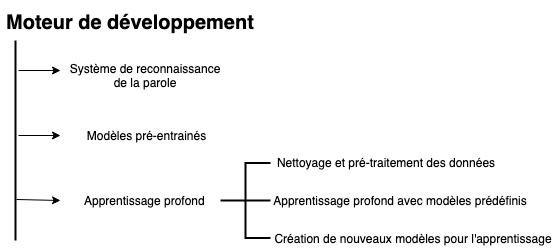
\includegraphics[width=400pt]{images/chap3/Pipeline_moteur_V1.png}
     \caption{Principales fonctions de l'environnement de développement pour la reconnaissance de la parole}
     \label{pip_dev}
 \end{figure}

Nous détaillons dans le chapitre suivant les différents modules de l'environnement de développement ainsi que leur fonctionnement.


\section{Collecte et pré-traitement des données}
Afin d'entraîner un modèle pour la tâche de reconnaissance de la parole, de grandes ressources en terme de données sont requises. Nous nous sommes inspirés des travaux de \cite{e2earabiclexiconfree} afin d'accéder à des données utilisables pour l'apprentissage de notre modèle.\\
Avant de parler de l'extraction et du pré-traitement de ces données, il est important de définir les critères \cite{towardse2esr} que doivent remplir ces dernières pour l'apprentissage. Nos données doivent obligatoirement : 
\begin{itemize}
    \item contenir des enregistrements audio et les transcriptions qui y correspondent,
    \item être de l'arabe moderne standard et non pas un dialecte,
    \item contenir un minimum d'une vingtaine d'orateurs, et
    \item être d'une longueur d'au moins 500 heures de dialogue. \\
\end{itemize}

Pour la conception de notre solution, nous testons nos modèles sur différentes tailles de corpus comme nous l'expliquons dans la suite de ce chapitre. Ces corpus sont respectivement constitués de : six heures de dialogues, 60 heures de dialogue, 260 heures de dialogue et 1200 heures de dialogue. Nous nommons corpus d'essai les six heures de dialogue car la source de données pour ce corpus est différente de celle du reste des données; nous nommons ce second corpus corpus élargi. 

\subsection{Collecte du corpus d'essai}\label{corpus_essais}
Les six heures de dialogue du corpus d'essai furent une partie du corpus collecté par l'équipe QCRI\footnote{https://www.qcri.org} et est disponible en libre accès sur la plateforme Github \cite{qcri6}. De cette référence, nous tirons un fichier texte contenant une liste de liens où chacun correspond à un enregistrement audio. Il a donc fallu développer un algorithme d'extraction automatique pour télécharger ces enregistrements. Nous avons également accès à un fichier contenant la transcription associée à chaque enregistrement. \\
La figure \ref{QCRI6} résume ce processus d'extraction :

\begin{figure}[H]
    \centering
    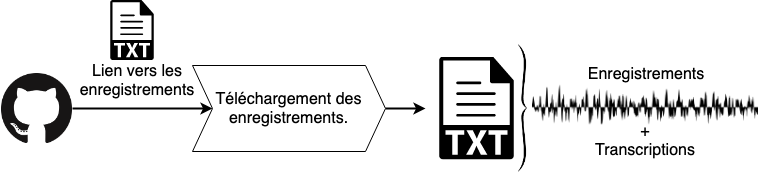
\includegraphics[height=140pt,width=450pt]{images/chap3/QCRI-6h-Github.png}
    \caption{Processus d'extraction des six heures de dialogue du corpus d'essai}
    \label{QCRI6}
\end{figure}

Le résultat est un corpus composé de 2219 enregistrements d'Arabe Moderne Standard (Modern Standard Arabic, MSA) enregistrés par une dizaine d'orateurs et où chaque enregistrement est d'une durée qui varie entre six secondes et une minute environ.

\subsection{Collecte des données du corpus élargi}\label{collecte_donnees}
Pour la suite de la conception du système, nous avons contacté l'équipe du QCRI qui nous ont accordé un accès au corpus MGB-2 \cite{mgb2corpus}. Ce corpus se compose de 1200 heures et plus d'une centaine d'orateurs de programmes enregistrés de la chaîne télévisée Al-Jazeera. La distribution des orateurs est diverse en terme de genre. La plupart de ces programmes sont des interviews de différentes personnalités et contiennent donc des questions. Il est très important pour nous que le corpus contienne des questions. En effet, \textit{ASeR-System} doit retranscrire ce type d'entrées pour qu'il soit testé, par la suite, avec un système de questions-réponses.  Tous les programmes ont été sous-titrés manuellement. 

Contrairement aux données du corpus d'essai, celles du corpus élargi sont formalisées d'une manière différente. La première chose que nous remarquons est les tailles des enregistrements qui sont d'une durée qui varie entre 25 et un peu plus d'une heure. La seconde est le format des fichiers qui contiennent les transcriptions qui sont au format XML suivant l'arborescence suivante : \\

\begin{figure}[H]
    \centering
    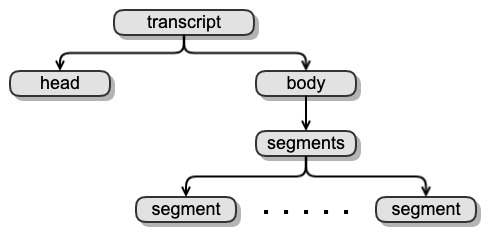
\includegraphics[height=150pt,width=325pt]{images/chap3/xml.jpg}
    \caption{Structure des fichiers XML du corpus élargi contenant les transcriptions}
    % Ancien Titre : Format des fichiers XML contenant les transcriptions
\end{figure}

Afin de tirer partie de ces données, un pré-traitement est nécessaire. Nous découpons ce pré-traitement en : 
\begin{itemize}
    \item extraction des temps de début et de fin de chaque phrase prononcée par un orateur à partir du fichier XML,
    \item extraction de la transcription associée à chaque phrase prononcée par un orateur,
    \item découpage des enregistrements audio selon les temps de début et de fin de phrase, et
    \item constitution d'un corpus contenant des enregistrements de durée allant de 6 à 40 secondes environ ainsi que la transcription qui y est associée sous forme de fichiers texte. \\
\end{itemize}

L'algorithme \ref{algo1} résume l'opération de collecte de données à partir du corpus élargi : 


\begin{algorithm2e}[H]
\SetAlgoLined
\label{ext_trans}
\SetKwInOut{Input}{Input}
\SetKwInOut{Output}{Output}
\Input{     repertoire\_dataset}
\tcc{repertoir\_dataset : le chemin vers le répértoire du dataset}
\Output{\tcc{Pas de variables en Output}}
\BlankLine
 liste\_pairs\_audio\_transcriptions $\gets$ liste\_fichiers(repertoire\_dataset) \\
 \For{(audio, fichierXML) $\in$ liste\_pairs\_audio\_transcriptions}{
    \For{segment $\in$ fichierXML}{
        date\_debut $\gets$ attribut\_start\_time \\
        date\_fin $\gets$ attribut\_end\_time \\
        transcription $\gets$ generer\_transcription(segment) \\
        liste\_transcriptions.ajouter(trancription)
        }
    generer\_fichier\_transcriptions(liste\_transcriptions) \\
    liste\_enregistrements\_audio $\gets$ Decouper\_audio(audio, date\_debut, date\_fin)\\
    generer\_fichier\_audio( liste\_enregistrements\_audio) 
    }
\caption{Extraction des transcriptions et partitionnement des longs enregistrements \label{algo1}}
\end{algorithm2e}

Maintenant que nous avons ces données à notre disposition, nous pouvons passer au pré-traitement pour qu'elles puissent être utilisées lors de l'apprentissage de nos modèles.

\subsection{Pré-traitement des données}
\subsubsection{Extraction des caractéristiques des enregistrements}\label{mfcc_section}
Afin d'utiliser nos enregistrements audio pour la phase d'apprentissage, nous devons extraire les caractéristiques de ces derniers. Il existe différentes manières d'effectuer cette opération mais dans le cadre de la reconnaissance de la parole nous nous intéressons aux caractéristiques MFCC. MFCC est l'acronyme de Mel Frequency Ceptral Coefficient introduit dans les années 1980s \cite{mfccintro}. Le processus par lequel il faut passer pour obtenir les caractéristiques MFCC est le suivant :
\begin{enumerate}[label=(\roman*)]
    \item Le signal audio passe par un filtre de pré-accentuation pour être découpé en un ensemble de spectres (qui peuvent être considérés comme des images ou plutôt des trames).
    \item Une transformation de fourrier est ensuite appliquée à chaque image afin de calculer les fréquences des spectres qui sont appelés périodogrammes.
    \item Calcul des Filter Bank\footnote{Filter Bank : Ensemble de 40 filtres appliqués aux periodogrammes pour extraire les bandes de fréquences.} est effectué pour y appliquer ensuite une Transformée en Cosinus Discrète (TCD) aux groupes de filtres en conservant un certain nombre de coefficients résultants tandis que les autres sont ignorés.
    \item L'étape finale consiste à normaliser les valeurs de ces coefficients.\\
\end{enumerate}

Dans notre cas, après application du MFCC sur nos données, chaque enregistrement audio sera représenté par une matrice de 40 colonnes où chaque colonne est une caractéristique et chaque ligne est une partie du spectrogramme; nous appelons cette partie timestep. Cette matrice n'étant pas normalisée, nous passons par une étape de normalisation.

\subsubsection{Normalisation des spectrogrammes}\label{normalisation_section}
La normalisation des données est une phase quasi nécessaire pour toute tâche d'apprentissage automatique et notre problématique ne fait pas exception à la règle.\\
Il existe plusieurs méthodes pour normaliser un jeu de données; nous nous intéressons à la méthode \textit{Min-Max} qui consiste à calculer les valeurs minimum et maximum de chaque attribut du jeu de données pour ensuite appliquer la formule : 

    \begin{equation}
            Normalise(X_{i}) = \frac{X_{i} - Min(X)}{Max(X) - Min(X)}
            \label{normalisation_equation}
    \end{equation}
    où :\\ \\
    X : est un attribut du spectrogramme, et \\
    $X_{i}$ : une valeur de X que nous voulons normaliser.

Dans le cas de notre problématique, le but de cette normalisation est de contenir toutes les valeurs entre 0 et 1 pour assurer une meilleure mise à jour des poids des réseaux de neurones lors de l'apprentissage.

\subsubsection{Pré-traitement des transcriptions}\label{trans_preprocessing}

Le second volet de nos données est l'ensemble des transcriptions. Chaque transcription est un texte écrit en utilisant la translittération Buckwalter \cite{buckwalter}. Cette translittération définit un mapping non ambigu de représentation de texte arabe en caractères latins étendus et vice-versa. La première étape du pré-traitement consiste à remplacer les caractères présents dans les transcriptions et qui ne font pas partie de l'alphabet Buckwalter. Ces caractères sont les suivants : 
\begin{itemize}
    \item les nombres présents sous la forme de nombres arabes (écrits en graphie occidentale ou orientale) qu'il faut convertir en texte,
    \item le cas particulier des lettres de l'alphabet où certaines lettres qui devraient être en minuscule selon la table Buckwalter sont écrites en majuscule et où une conversion est nécessaire,
    \item le caractère "\%" qui doit être remplacé par des caractères alphabétiques, ainsi que
    \item les caractères "\#", ";", "@" et "\textbackslash \textbackslash" qui n'apparaissent qu'un nombre dérisoire de fois sur tout le jeu de données.\\
\end{itemize}

Ce traitement des caractères spéciaux est important car des caractères superflus et sémantiquement redondants mais syntaxiquement différents augmentent la dimensionnalité des transcriptions. Ceci peut résulter par la suite en un sous-apprentissage. Notons ici, qu'a fin de pouvoir utiliser ces transcriptions lors de l'apprentissage, une conversion vers des valeurs numériques est requise. De ce fait nous présentons deux types d'encodage : encodage basé caractères et encodage basé mots.

\subsubsection{Encodage des transcriptions basé caractères} \label{character_based}
La première étape de cet encodage consiste à attacher au début de la transcription le caractère spécial "\textbackslash t" et le caractère spécial "\textbackslash n" pour marquer le début et la fin de transcription, respectivement.

La conversion de chaque caractère en valeur numérique se fait en utilisant une table de mappage qui associe à chaque caractère une valeur selon l'ordre d'apparition de celui-ci dans le corpus de transcriptions. Maintenant que chaque transcription est sous forme de valeurs numériques, nous appliquons un encodage appelé \textit{One Hot Encoding} \cite{textencoding} qui consiste à représenter chaque transcription sous forme de matrice binaire où chaque ligne représente un caractère de la transcription et où chaque colonne représente un caractère du jeu de caractères du corpus. Il s'agira par la suite de mettre à 1 chaque croisement de caractères entre lignes et colonnes. Pour illustrer cet encodage nous prenons l'exemple suivant : 

Soit le jeu de caractères "a", "b", "x", "d", "e", "l", "o", "h", "r", "w", " " et la phrase "hello world" que nous voulons encoder. La figure \ref{One-hot-car} montre l'encodage One Hot de cette phrase.

\begin{figure}[H]
    \centering
    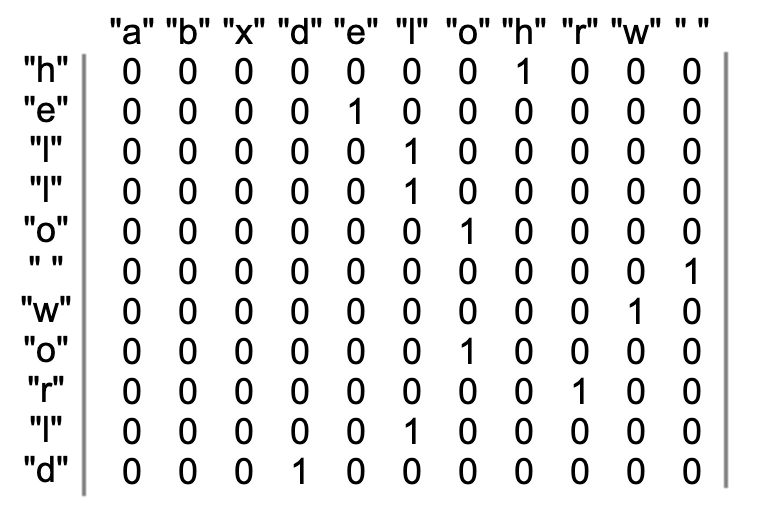
\includegraphics[height=200pt,width=300pt]{images/chap3/matrice_one_hot.png}
    \caption{Exemple de l'encodage basé caractères appelé One Hot Encoding}
    \label{One-hot-car}
\end{figure}

L'algorithme \ref{algo2} résume l'encodage basé caractères des transcriptions :

\begin{algorithm2e}[H]
\SetAlgoLined
\SetKwInOut{Input}{Input}
\SetKwInOut{Output}{Output}
\Input{repertoire\_dataset \\ char\_to\_int\_characters : table de conversion des caractères vers des entiers}
\Output{\tcc{Pas de variables en Output}}
\BlankLine
 liste\_transcriptions $\gets$ recuperer\_transcriptions(repertoire\_dataset) \\
 \For{transcritpion $\in$ liste\_transcriptions}{
    \For{index, caractere $\in$ transcription}
    {
        encoder\_caractere\_en\_input() \\
        \If{index > 1}{
            encoder\_caractere\_en\_target()} \\
    }
    decoder\_input.ajouter(caractere\_encode\_en\_input) \\
    decoder\_target.ajouter(caractere\_encode\_en\_target)
    }
 enregistrer\_fichier(decoder\_input) \\
 enregistrer\_fichier(decoder\_target)
 \caption{Encodage basé caractères des transcriptions \label{algo2}}
 \label{enc_car}
\end{algorithm2e}

L'encodage basé caractères est simple à implémenter mais présente des résultats qui sont moins performants qu'un encodage basés mots. En effet, des erreurs dans les suites de caractères donneraient naissance à des mots qui n'existent pas. C'est pour cela qu'il faut y associer un modèle de langage pour corriger ces erreurs. L'encodage basé mots quant à lui, en plus de présenter des résultats plus cohérents que ceux de l'encodage basé caractères, fait office de modèle de langage en assurant que les suites de caractères sont correctes pour les mots prédits correctement.

Nous présentons dans ce qui suit les différentes approches pour l'encodage basé mots.
 

\subsubsection{Encodage des transcriptions basé mots}\label{word_based}
Tout comme pour l'encodage basé caractères, nous attachons au début de nos transcriptions le mot spécial SOS qui signifie "Start Of Sentence" et à la fin le mot EOS qui signifie "End Of Sentence" pour marquer respectivement le début et la fin d'une transcription.

L'encodage basé mots va vraisemblablement présenter des résultats très différents de l'encodage basé caractères et ce car le modèle devra distinguer et classifier un très grand nombre de mots en comparaison avec une cinquantaine de caractères pour le premier encodage. 

Pour encoder des mots,  nous pensons naturellement à l'encodage \textit{One Hot Encoding} également appelé \textit{Bag Of Words} dans le cas des mots. C'est une approche similaire à celle présentée dans la section  \ref{character_based} et qui consiste à représenter une transcription par une matrice où les lignes représentent les mots, séparés par le caractère blanc, et les colonnes représentent tous les mots distincts de notre jeu de données. Nous illustrons cet encodage par un exemple réel de notre jeu de données. Prenons la phrase "m\$AhdynA AlkrAm AlslAm Elykm" qui est la translittération de "\setcode{utf8}\<مشاهدينا الكرام السلام عليكم>" dont l'encodage est le suivant :  

\begin{figure}[H]
    \centering
    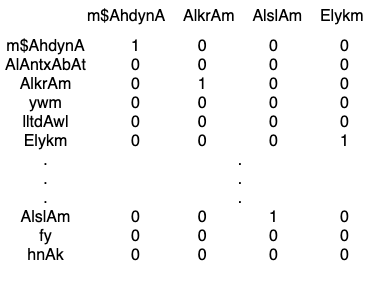
\includegraphics[height=200pt,width=300pt]{images/chap3/One-Hot-Word-level.png}
    \caption{Exemple de l'encodage basé mots Bag Of Words}
    \label{exemple_bag_of_words}
\end{figure}

Cet encodage paraît adéquat à première vue mais pour un jeu de données aussi large que le notre où il existe plus de 150000 mots distincts, il est quasi-impossible, en terme de mémoire vive, d'encoder chaque transcription \textit{x} sous forme d'une matrice de taille (x, 150000) d'où l'impossibilité d'utiliser cet encodage pour notre dataset.

Il existe néanmoins un autre encodage qui est l'encodage binaire où nous convertissons chaque mot en vecteur binaire. Cet encodage s'effectue en suivant les étapes suivantes :
\begin{itemize}
    \item Collecte de la liste des mots distincts existant dans notre jeu de données.
    \item Création d'une table associant un indice unique à chaque mot.
    \item Création d'un vecteur binaire avec une taille suffisante pour encoder chaque indice tel que :
    \begin{equation}
        2^{x} < nbr\_mots\_distincts
    \end{equation}
    où :\\ \\
    $x$ est le nombre de bits du vecteur.
    Nous estimons ne pas avoir besoin de plus de 18 bits pour encoder chaque mot de notre jeu de données.
    \item Convertir l'indice de chaque mot en binaire et l'introduire dans le vecteur binaire. \\
\end{itemize}

Si nous prenons l'exemple précédent avec la phrase : "m\$AhdynA AlkrAm AlslAm Elykm", l'encodage de cette dernière serait le suivant : 

\begin{figure}[H]
    \centering
    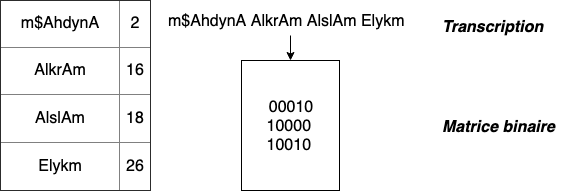
\includegraphics[width=400pt]{images/chap3/Binaire.png}
    \caption{Encodage binaire des mots du jeu de données}
\end{figure}

Bien que l'encodage binaire semble apporter la solution à notre problématique, il présente un désavantage majeur lors de l'apprentissage qui est le calcul d'une fausse précision. Si pour un vecteur binaire le modèle nous affiche, par exemple, une précision de 90\%, notre modèle aura donc la faculté de prédire 9 bits sur 10 mais après reconversion du vecteur binaire prédit en mot nous nous rendrons compte que le mot deviendra un tout autre mot.

Afin de remédier à cette anomalie, nous présentons un nouvel encodage pour les mots. Le principe de cet encodage consiste à :
\begin{itemize}
    \item calculer le nombre maximum de caractères par mot dans notre jeu de données,
    \item pour les transcriptions en entrée du modèle d'apprentissage, encoder chaque mot d'une transcription par un vecteur de taille \textbf{\og Nombre de caractères du jeu de données $\times$ Nombre maximum de caractères par mot \fg} de telle sorte à encoder chaque caractère de chaque mot en utilisant un One Hot Encoding sur une partie de taille \textbf{{Nombre de caractères du jeu de données}} de ce vecteur, et
    \item pour les transcriptions en sortie du modèle d'apprentissage, encoder chaque mot de la transcription par \textbf{N} vecteurs où \textbf{N} représente le \textbf{nombre maximum de caractères par mot} et où chaque vecteur est de taille \textbf{\og Nombre de caractères du jeu de données \fg}.\\ 
\end{itemize}

Afin de clarifier cet encodage qui peut paraître inhabituel au premier abord, nous présentons un exemple d'encodage avec le mot "hello", le jeu de caractères "a", "e", "h", "l", "b", "x", "o", " " et la taille maximale de mots de 7 comme le montre la figure \ref{word_based_multiple_output}.

 \begin{figure}[H]
    \centering
    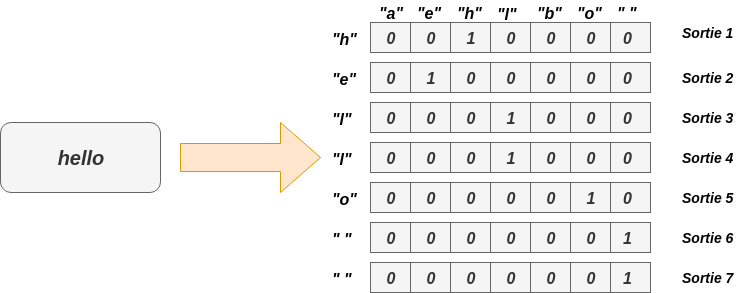
\includegraphics[height=175pt,width=350pt]{images/chap3/encodage_base_mots.png}
    \caption{Exemple Encodage basé mots à plusieurs sorties}
    \label{word_based_multiple_output}
\end{figure}

L'algorithme \ref{algo3} suivant résume cet encodage :

\begin{algorithm2e}[H]
\SetAlgoLined
\SetKwInOut{Input}{Input} 
\SetKwInOut{Output}{Output} 
\Input{repertoire\_dataset \\ char\_to\_int\_characters : table de conversion des caractères vers des entiers \\ max\_car\_mot : maximum de caracteres par mot de tout le corpus \\ nb\_car : nombre de caracteres disctincts du corpus}
\Output{\tcc{Pas de variables en Output}}
\BlankLine
liste\_transcriptions $\gets$ recuperer\_transcriptions(repertoire\_dataset) \\
\For{transcritpion $\in$ liste\_transcriptions}{
    liste\_mots $\gets$ diviser\_transcription\_en\_mots(transcription) \\
    \For{ mot $\in$ liste\_mots}{
        longueur\_liste $\gets$ nb\_car $\times$ max\_car\_mot \\
        encoded\_word $\gets$ liste\_de\_zeros(longueur\_liste) \\
        encoded\_word\_target $\gets$ matrice\_de\_zeros(nbr\_car, max\_car\_mot) \\
        \For{i, index\_caractere $\in$ mot}{
            encoder\_caractere\_en\_input()\\
            \If{i<max\_caracteres\_par\_mot}{
                encoder\_fin\_mot\_input()
                \If{i > 1}{
                encoder\_caractere\_en\_target() \\
                } 
            }
        }
        
    }
    encoded\_input.ajuoter(encoded\_transcriptions\_input) \\
    encoded\_target.ajouter(encoded\_transcriptions\_target) 
}
enregistrer\_fichier(decoder\_input) \\
enregistrer\_fichier(decoder\_target) 
\caption{Encodage basé mots des transcriptions \label{algo3}}
\label{enc_mot}
\end{algorithm2e}

En adoptant un tel encodage, nous évitons les difficultés liées à la gestion de la mémoire ainsi que l'erreur entre la précision et le WER pour l'encodage binaire. Nous présentons dans le chapitre suivant l'implémentation d'un tel encodage ainsi que les performances achevées par ces deux encodages. 

\subsubsection{Teacher Forcing}
Afin de mettre en place l'architecture que nous présentons dans la suite de ce chapitre, nous aurons, en plus des transcriptions encodées, une copie encodée de ces transcriptions à l'instant t+1. Ce principe s'appelle Teacher Forcing \cite{teacherforcing}, également appelé Professor Forcing. Cela permet à notre système de déduire quel caractère/mot avoir en sortie sachant  l'enregistrement audio et la séquence de caractères/mots précédents.

\subsubsection{Traitement des grandes tailles de données}
Comme mentionné précédemment, nous aurons à effectuer notre apprentissage sur des jeux de données de tailles différentes afin d'évaluer les performances des différents modèles. Nous serons donc amenés à effectuer des apprentissages sur six heures, 60 heures, 260 heures et 1200 heures d'enregistrements audio en fin de parcours.

Gérer une telle quantité de données nous met face à deux problèmes principaux : 
\begin{itemize}
    \item impossibilité de charger le dataset nettoyé en mémoire pour l'encodage des transcriptions au vue de sa taille, et
    \item envoi de toutes les données à notre modèle pour l'apprentissage sachant que dix heures de dialogue équivaut à environ 500 Mo en mémoire. \\
\end{itemize}

Afin de remédier à ces complications, nous appliquons le principe de pagination. Nous commençons par la génération des fichiers binaires qui contiennent les spectrogrammes ainsi que leurs transcriptions. Au lieu de générer un fichier contenant toutes les données à notre disposition, nous générons un ensemble de fichiers en limitant le nombre d'heures de dialogue contenues dans chaque fichier. Nous prenons, pour la suite de ce projet, des fichiers de dix heures de dialogue chacun.

L'étape suivante consiste à créer à partir de ces partitions, des sous-partitions de telle sorte à avoir des fichiers binaires pour l'apprentissage et le test. Nous définissons ce nombre de sous-partitions de manière dynamique de telle sorte à avoir une utilisation minimum de la mémoire vive de l'utilisateur. Nous calculons le nombre de partitions à partir de la formule suivante : 
\begin{equation}
    nbr\_partitions = \frac{32}{memoire\_utilisateur} * duree\_dataset\_heures
\end{equation}

Nous rencontrons une difficulté supplémentaire lors de l'apprentissage car nous devons envoyer toutes nos données à notre modèle pour qu'il puisse effectuer la mise à jour des poids sur l'ensemble de données mais là nous ne pouvons avoir toutes nos données en mémoire. C'est ici que nous faisons appel au principe de générateur de données qui se définit par les étapes suivantes : 

\begin{itemize}
    \item création d'une fonction chargeant en mémoire, à tour de rôle, les couples de fichiers contenant les spectrogrammes et transcriptions,
    \item création d'une table de hachage contenant comme clé les couples de nombre de timesteps des spectrogrammes et transcriptions, et comme valeur une liste des spectrogrammes et transcriptions ayant ces tailles, et
    \item envoi successif des listes de chaque clé à la fonction d'apprentissage.
\end{itemize}

Nous avons donc implémenté manuellement l'envoi des données à la fonction d'apprentissage pour permettre une gestion optimale de la mémoire en premier lieu et d'accélérer l'apprentissage en second lieu.

Maintenant que notre corpus est extrait et pré-traité nous passons à la conception des différentes architectures de modèles pour notre système.


\section{Apprentissage du système}\label{apprentissage}
Nous nous attelons dans cette partie à la conception du modèle de notre système de reconnaissance de la parole. Comme mentionné précédemment, nous développons un système End-To-End qui, contrairement à l'approche basée reconnaissance de phonèmes, consistera en un module prenant en entrée un enregistrement audio et fournissant en sortie la transcription qui lui correspond. Dans le cas de la reconnaissance de la parole, nous avons affaire à des données de type séries temporelles où la taille de chaque enregistrement est variable. Comme tout exercice d'apprentissage, il existe plusieurs modèles et plusieurs architectures pour appréhender le problème. Pour les séries temporelles, nous nous intéressons aux modèle de type Séquence à Séquence.

\subsection{Séquence à Séquence et Encodeur/Décodeur}
Le modèle Séquence à Séquence, traduit de l'anglais Sequence to Sequence, fut introduit en 2014 par Google \cite{seq2seqgoogle}. Ce modèle a pour but de mapper une entrée avec une sortie et où la longueur des entrées et celle des sorties peuvent être différentes.

Par exemple, traduire "What are you doing today ?" de l'anglais vers le français comporte une entrée de 5 mots et une sortie de 4 mots "Que faites-vous aujourd'hui ?". Comme les tailles des entrées et sorties sont différentes, ce qui est le cas pour les problèmes à données sous forme de séquences, nous ne pouvons utiliser un architecture séquentielle classique pour mapper chaque mot de la phrase en anglais à la phrase en français. Le modèle séquence à séquence est utilisé pour traiter des problèmes comme celui-ci.

Le modèle séquence à séquence se base sur le principe sous-jacent d'encodeur/décodeur \cite{encdecdef} que nous représentons par l'illustration suivante :
\begin{figure}[H]
    \centering
    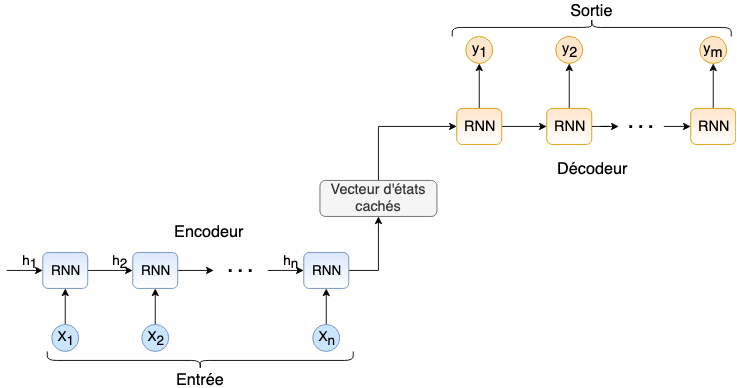
\includegraphics[height=200pt,width=400pt]{images/chap3/EncDec.png}
    \caption{Architecture de base d'un encodeur/décodeur}
    \label{Enc_Dec}
\end{figure}

Comme illustré dans la figure \ref{Enc_Dec}, le modèle comprend deux blocs principaux qui sont l'encodeur et le décodeur ainsi qu'un vecteur intermédiaire qui est le vecteur d'états cachés.


\subsubsection{Encodeur}
L'encodeur est le premier bloc de ce modèle et est composé d'une pile de plusieurs unités récurrentes. Chacune de ces unités ne prend qu'un timestep de la séquence d'entrée et collecte les informations relatives à cet élément que nous appelons état caché (hidden state en anglais) et qui se calcule à partir de la formule suivante :

\begin{equation}
    h_{t} = f(W^{(hh)}h_{t-1} + W^{(hx)}x_{t})
\end{equation}
    où :\\ 
    h : est l'état caché à timestep \textit{t}. \\
    x : est la donnée à un pas de temps \textit{t}. \\
    $W^{(hh)}$ : représente les poids relatifs l'état caché.\\
    $W^{(hx)}$ : représente les poids relatifs à la sortie de l'encodeur.

L'encodeur a pour but de donner une représentation de la séquence de données afin de "l'encapsuler" dans le vecteur d'états cachés (Hidden States Vector en anglais), et va donc contenir l'état caché final produit par l'encodeur du modèle qui fera office d'état initial pour le décodeur.

Dans le cadre de notre projet, l'encodeur est la partie du modèle qui prend les enregistrements audio en entrée et apprend à regrouper les séquences d'un spectrogramme et produire une représentation vectorielle de celle-ci.

\subsubsection{Décodeur}
Tout comme l'encodeur, le décodeur se compose d'un ensemble d'unités récurrentes \cite{encoderdecoder} où : 
\begin{itemize}
    \item chaque unité prédit une sortie \textbf{$Y_{t}$} pour un pas de temps \textbf{t}, et
    \item chaque unité prend en entrée la donnée et un vecteur d'état caché de l'unité précédente (ou de l'encodeur si c'est la première unité) et génère à partir de cela un output et son propre vecteur d'états cachés pour l'unité suivante.\\
\end{itemize}

Le calcul de l'état caché se fait à partir de la formule suivante :

\begin{equation}
    h_{t} = f(W^{hh}h_{t-1})
\end{equation}
    où :\\ 
    h : est l'état caché à un pas de temps t. \\
    $W^{(hh)}$ : représente les poids du réseau.
    
et l'output {$Y_{t}$} de l'unité récurrente pour un pas de temps \textbf{t} est calculé à partir de l'état caché selon la formule suivante :
\begin{equation}
    Y_{t} = Softmax(W^{s}h_{t})
\end{equation}
où :\\
    Y : est l'output de l'encodeur à un pas de temps t. \\
    h : est l'état caché à un pas de temps t. \\
    W : représente les poids du réseau. \\
    \textit{Softmax} : est une fonction d'activation qui attribue des probabilités décimales à chaque classe d'un problème à plusieurs classes. La somme de ces probabilités décimales doit être égale à 1 \cite{softmax}.

\subsection{Discussion}
L'intérêt du modèle encodeur/décodeur réside dans le fait de pouvoir associer des séquences de différentes longueurs en entrée et en sortie. Nous utilisons ce modèle pour le développement du système où :
\begin{itemize}
    \item les entrées de l'encodeur sont nos enregistrements audio,
    \item les entrées du décodeur sont les transcriptions, et
    \item les sorties du décodeur sont les transcriptions à \textit{t+1} selon le principe de Teacher Forcing que nous détaillons dans le chapitre suivant. \\
\end{itemize}

Nous passons à présent à la conception de l'architecture interne des unités récurrentes de notre modèle.

\section{Architecture du modèle}
Il existe plusieurs architectures possibles pour le développement de notre modèle, comme nous l'avons noté dans l'état de l'art. Chaque travail trouvé dans l'état de l'art présente une conception, un corpus et bien évidement des résultats différents, ce qui peut prêter à confusion.

Afin de mettre en place l'architecture idéale pour notre modèle, nous en expérimentons deux et pour chaque architecture nous prenons en compte deux variantes. Nous comparons ensuite l'évolution des courbes d'apprentissage de chaque architecture. Afin que notre système soit améliorable, il doit pouvoir prendre en compte l'augmentation (ou même la réduction) du volume de données. Ainsi, pour que cette comparaison soit précise, nous utilisons quatre jeux de données : six heures de dialogue, 60 heures, 260 heures et 1200 heures de dialogue.

Avant de présenter nos architectures nous commençons par présenter les couches que nous utilisons.

\subsection{Présentation des couches utilisées}
\subsubsection{Long Short-Term Memory}
Long-Short-Term-Memory, ou LSTM, sont un type particulier de RNNs et ont été introduits par \cite{lstmdef}. Les LSTMs ont été conçus pour éviter le problème de dépendance à long terme. En effet, il s'est avéré que les RNNs ne peuvent apprendre le séquencement d'informations à long terme. Comprendre et se souvenir du séquencement des informations quelque soit la taille de la séquence est l'avantage des LSTMs par rapport aux RNNs, et ce grâce au mécanisme des portes présentes dans une cellule LSTM. Ces portes peuvent apprendre les données importantes à conserver parmi les données d'entrée. En faisant cela, un LSTM peut transmettre des informations pertinentes tout au long de la séquence de données pour effectuer des prédictions.

La figure \ref{LSTM} présente le contenu d'une cellule LSTM ainsi que les opérations internes qu'y s'effectuent : 

\begin{figure}[H]
    \centering
    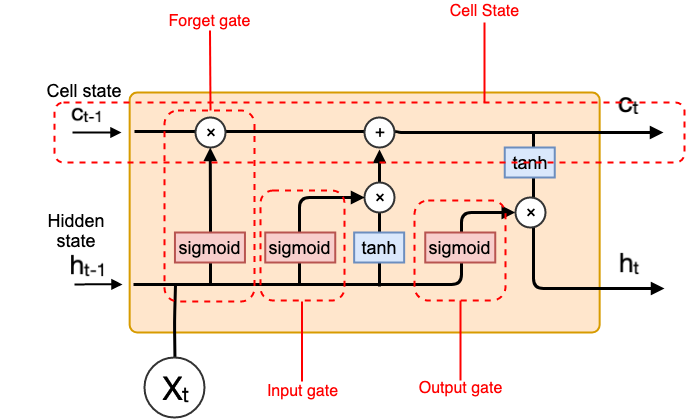
\includegraphics[height=190pt,width=325pt]{images/chap3/LSTM.png}
    \caption{Contenu d'une cellule LSTM \cite{LSTM_cell}}
    \label{LSTM}
\end{figure}

Comme le montre la figure \ref{LSTM}, en plus du Hidden State qu'on retrouve dans une cellule RNN, il y a le Cell State qui est le concept de base des LSTMs. Le Cell State permet de garder en mémoire les informations pertinentes. Ces informations sont donc sauvegardés grâce aux trois portes d'une cellule LSTM \cite{lstmgates} qui sont :

\begin{itemize}
    \item \textbf{Forget Gate} : pouvant être traduite en porte d'oubli, elle décide quelles informations doivent être conservées. Pour se faire, les informations contenus dans le vecteur d'états cachés précédent et les données en entrée sont additionnées et passent par la fonction sigmoïde et la valeur résultante est comprise entre 0 et 1. Plus la valeur se rapproche de 1 plus l'information est pertinente.\\
    \item \textbf{Input Gate} : L'input Gate, ou porte d'entrée, permet de mettre à jour le Cell State. Les valeurs du vecteur d'états cachés précédent et celles des donnée en entrée sont additionnées et passent par une fonction sigmoïde ce qui, comme pour la Forget Gate, permet de désigner les données pertinentes. En plus de la fonction sigmoïde, ces mêmes informations passent par une fonction tanh pour rendre les valeurs entre -1 et 1 afin de contribuer à la régulation du réseau. Les sorties de la fonction sigmoïde ainsi que tanh sont multipliées et ce résultat est additionné à la valeur contenue dans le Cell State.\\
    \item \textbf{Output Gate} : l'Output Gate, ou porte de sortie, décide quel devrait être le prochain vecteur d'états cachés. Premièrement, nous passons l'état caché précédent et l'entrée actuelle dans une fonction sigmoïde. Ensuite, nous passons le Cell State mis à jour par la fonction tanh. Nous multiplions la sortie tanh par la sortie sigmoïde pour décider quelles informations l'état caché doit contenir. C'est ainsi que sont générés les nouveaux Cell State et Hidden State qui seront utilisés pour le timestep suivant.
\end{itemize}
        
\subsubsection{Gated Reccurent Unit}
Introduit en 2014 par \cite{GRUpaper}, les Gated Reccurent Units (GRU) sont des unités récurrentes assez similaires à des LSTMs dans leur fonctionnement. Les principales différences sont que les GRUs n'ont pas de Cell State pour transferer l'information et n'ont que deux portes \cite{lstmgates} : 
\begin{itemize}
    \item \textbf{Update Gate} : agit de manière similaire aux Forget Gate et Input Gate d’un LSTM. Cette porte décide quelles informations doivent être gardées et quelles nouvelles informations ajouter; et
    \item \textbf{Reset Gate} : utilisée pour décider de la quantité d'informations à oublier.\\
\end{itemize}

La figure \ref{GRUU} présente le contenu d'une unité GRU ainsi que les opérations internes qu'y s'effectuent.

\begin{figure}[H]
    \centering
    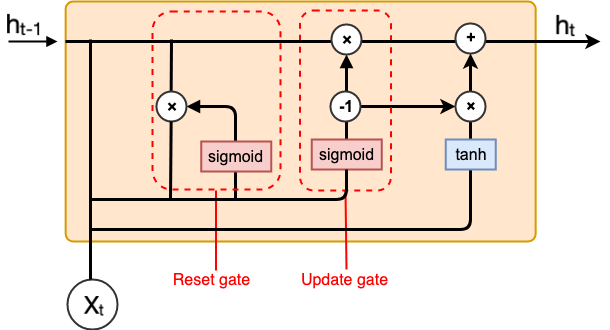
\includegraphics[height=185pt,width=325pt]{images/chap3/GRU.png}
    \caption{Contenu d'une cellule GRU}
    \label{GRUU}
\end{figure}

Les GRUs effectuent moins de calculs matriciels que les LSTMs et sont donc un peu plus rapides lors de l'apprentissage.

\subsubsection{Couches récurrentes bidirectionnelles}
Les couches récurrentes bidirectionnelles sont une extension des RNNs traditionnels qui peuvent améliorer les performances du modèle en cas de problème de classification de séquences \cite{bilstmdef}. Dans les problèmes où tous les timesteps de la séquence d'entrée sont disponibles, comme le cas de notre problème, les RNNs bidirectionnels entraînent deux RNNs au lieu d'un seul. Le premier de ces RNN accomplit un apprentissage sur la séquence d'entrée de la manière usuelle tandis que le second le fait sur une copie triée dans le sens inverse de la séquence d'entrée. Cela peut fournir un contexte supplémentaire au réseau et permettre un apprentissage plus plus complet. Pour notre problématique, ce type de couches joue le rôle d'un modèle de langage. 

\subsection{Architectures de l'approche End-To-End pour ASeR-Sytem}
Nous présentons dans cette partie les deux architectures où chaque architecture est basée sur un modèle encodeur/décodeur avec des RNNs mais aussi une variante à base de RNNs bidirectionnels pour chacune des deux architectures.

\subsubsection{Architecture de base}
Le modèle de base se compose de :
\begin{itemize}
    \item \textbf{Encodeur} : composé d'une couche récurrente et renvoie les vecteur Hidden State.
    \item \textbf{Décodeur} : composé de plusieurs couches récurrentes.
    \item \textbf{Couche Fully Connected} : Dernière couche du modèle d'un réseau de neurones MLP complètement connecté qui prend en entrée l'output du décodeur. \\
\end{itemize}

La figure \ref{Baseline} résume l'architecture de ce modèle.
\begin{figure}[H]
    \centering
    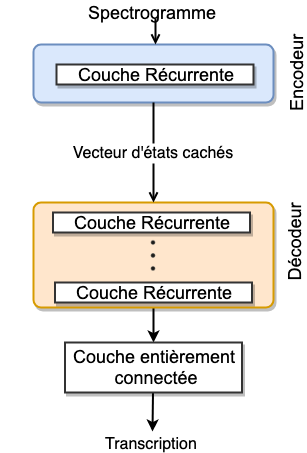
\includegraphics[height=240pt]{images/chap3/baseline_model.png}
    \caption{Architecture de base de ASeR-System}
    \label{Baseline}
\end{figure}

\subsubsection{Architecture avec couches convolutionnelles}
Le modèle à couches convolutionnelles se compose de :
\begin{itemize}
    \item \textbf{Couches convolutionnelles} : Se compose d'un ensemble de convolutionnelles et couches Pooling. Cette partie du modèle a pour but d'extraire les informations pertinentes du spectrogramme et de supprimer le bruit qui aurait échapper aux filtres du MFCC. La dernière couche génère des spectogrammes modifiés qui seront injectés en entrée de l'encodeur.
    \item \textbf{Encodeur} : composé d'une couche récurrente et renvoie le vecteur Hidden State.
    \item \textbf{Décodeur} : composé de plusieurs couches récurrentes. En plus de cela, le décodeur comporte une couche Dropout qui a pour but de minimiser les risques de sur-apprentissage en désactivant aléatoirement certains neurones des couches précédentes.
    \item \textbf{Couche Fully Connected} : Dernière couche du modèle, prend en entrée l'output du décodeur. \\
\end{itemize}

La figure \ref{arch_cnn} résume l'architecture du modèle.
\begin{figure}[H]
    \centering
    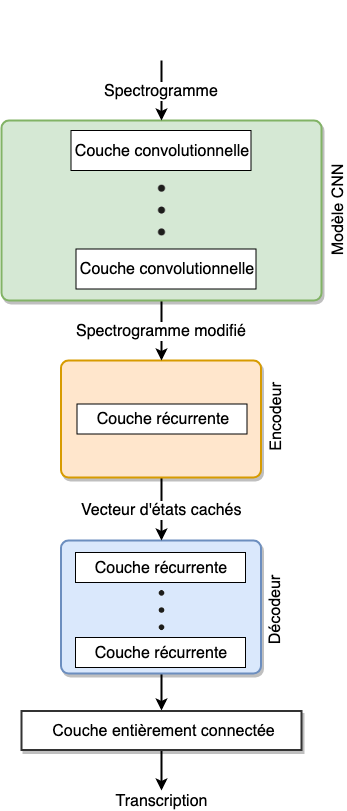
\includegraphics[height=340pt]{images/chap3/CNN_model.png}
    \caption{Architecture de ASeR-System avec couches convolutionnelles}
    \label{arch_cnn}
\end{figure}

\section{Utilisation du modèle d'apprentissage pour la reconnaissance}\label{inference}
Après l'apprentissage de notre modèle, nous devrons tester celui-ci sur des données de test dans un premier temps ensuite des données réelles ou, autrement dit, tester nos propres enregistrements audio. Contrairement à un modèle d'apprentissage classique, le modèle séquence à séquence ne fait pas une simple prédiction de classes qui, dans notre cas, nécessiterait l'enregistrement audio et sa transcription en entrée du modèle. C'est pour cela que nous effectuons une tâche d'inférence
\cite{modelinference}. Nous ne pouvons parler directement de prédiction car notre modèle se compose d'un encodeur et d'un décodeur. Le processus d'inférence se décompose en deux parties : la préparation du modèle après l'apprentissage et le décodage des transcriptions. La préparation du modèle se fait donc comme suit :

\begin{itemize}
    \item Chargement des couches d'entrée et états cachés de l'encodeur à partir du modèle après apprentissage.
    \item Chargement des couches d'entrées, couches récurrentes ainsi que couches de sortie du décodeur.
    \item Génération d'un modèle pour l'encodeur et un modèle pour le décodeur et ce à partir des couches chargés préalablement. \\
\end{itemize}

Maintenant que l'encodeur et le décodeur sont prêts, nous passons au décodage des transcriptions. Il est à noter que cette partie de l'inférence est sensiblement la même pour un encodage basé caractères ou encore un encodage basé mots. Les étapes sont les suivantes : 

\begin{itemize}
    \item Préparation de la table qui associe cette fois un entier à chaque caractère ou mot selon l'encodage.
    \item Prédiction du vecteur d'états cachés à l'aide de l'encodeur. Ce vecteur est la représentation de l'enregistrement audio en entrée.
    \item Prédiction du caractère ou du mot correspondant en donnant en entrée du décodeur le vecteur d'états ainsi que le caractère ou mot actuel, la sortie est le caractère ou mot prédit ainsi qu'un vecteur d'états qui sera en entrée de la prochaine prédiction. Si la prédiction effectuée est celle du premier caractère, le vecteur d'états est le vecteur d'états cachés généré par l'encodeur.
    \item Répéter l'étape précédente tant que le caractère ou mot généré n'est pas fin de transcription.
\end{itemize}

% Nous prenons un exemple réel pour illustrer le principe d'inférence avec la phrase : "yEtbr fyh AlEdyd mn xSwmkm AlsyAsyyn >n hnAk" ainsi qu'un encodage basé caractères. La figure ci-dessous résume les différentes étapes.

% \begin{figure}[H]
%     \centering
%     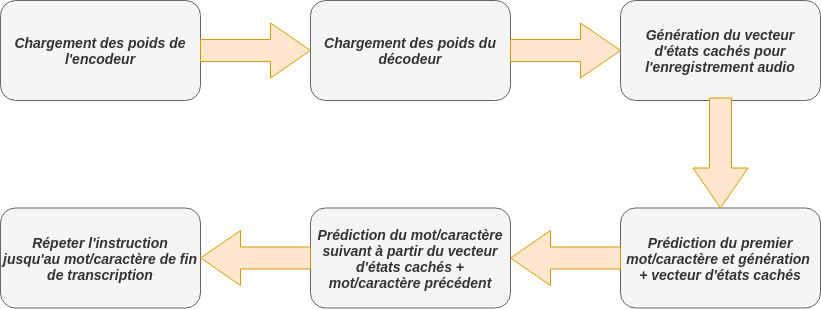
\includegraphics[width=400pt]{images/chap3/inference.png}
%     \caption{Étapes de l'inférence}
% \end{figure}


\section{Application de ASeR-System à un système de questions-réponses} \label{QASChap3}
 \textit{ASeR-System} peut être utilisé dans plusieurs domaines d'application du traitement automatique du langage naturel (TALN). Dans le cadre de ce projet, nous considérons les systèmes de questions-réponses comme domaine d'application. 

 L'équipe du LRIA, laboratoire de recherche en intelligence artificielle (Laboratory for Research in Artificial Inteligence) de l'université des sciences et de la technologie Houari Boumédiène a développé un système de questions-réponses nommé \textit{AFaQ-System} qui a été mis à notre disposition. Comme nous l'avons mentionné dans les sections \ref{QASdomain} et \ref{QASqstType}, un système de questions-réponses peut être classifié selon le domaine et/ou le type de questions qu'il accepte, le système de questions-réponses \textit{AFaQ-System} est de type factoïde, il répond aux questions qui commencent par :   \setcode{utf8}\< متى، كم، أين، من>. Un corpus \cite{QASCorpus} a été exclusivement développé dans le but d'être utilisé pour l'apprentissage des modèles des différents modules de ce système qui se compose de trois modules à savoir : 
 \begin{itemize}
     \item le module de pré-traitement d'une question (Question preprocessing),
     \item le module de pré-traitement des documents (document preprocessing), et
     \item le module d'extraction de réponses (answer extraction). \\
 \end{itemize}

La figure \ref{QAS_ASR} illustre la conception de l'application développée dans le cadre de ce projet. Cette application permet d'utiliser \textit{ASeR-System} avec \textit{AFaQ-System}.
 \begin{figure}[H]
    \centering
    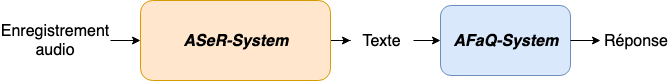
\includegraphics[width=400pt]{images/chap3/QASASR.png}
    \caption{Système de reconnaissance de la parole intégré avec un système de questions-réponses }
    \label{QAS_ASR}
\end{figure}

% dans la presentation on peut parler de l archi du modele sans trop détail : on parle vite fait sur les modules qui composent le QAS : Question processing, document processing et answer extraction 
% type du QAS : factoid (mata kam ayna et man)
% l accuracy par rapport à chaque question (confirmer avec guessoum)
% Le corpus sur le quel le tout à été testé (taille, type de question etc)  voir papier envoyer par aouichat 
% Comment le systeme de QR est integrer --> voir schéma



\section{Conclusion}
Dans de ce chapitre, nous avons présenté les données à notre disposition ainsi que le pré-traitement mis en place afin d'en tirer profit pour l'apprentissage de nos modèles. Ensuite, nous avons présenté au total quatre architectures basées sur le principe d'encodeur/décodeur mais qui se composent de couches différentes. Le but principal de ce choix de conception est de garantir l'implémentation d'un modèle fiable et performant. Pour finir, nous avons présenté \textit{AFaQ-System}, le système de questions-réponses que nous utilisons pour tester \textit{ASeR-System}.

Dans le chapitre suivant, nous passons à l'implémentation de nos modèle ainsi que le pré-traitement des données au vu des différentes phases d'apprentissage. Une fois le choix du modèle effectué sur la base de l'évolution des performance de chaque architecture, nous passerons à l'apprentissage du modèle final et au test de notre système à travers un système de questions-réponses.

\chapter{Réalisation de ASeR-System}
\section{Introduction}
Nous avons présenté précédemment les concepts de base d'un système de reconnaissance de la parole, les travaux qui ont présenté les résultats les plus performants ainsi que la conception de \textit{ASeR-System}, notre système End-To-End de reconnaissance de la parole pour la langue arabe. En plus d'effectuer la tâche de reconnaissance, \textit{ASeR-System} est un environnement de développement permettant d'intégrer le système de reconnaissance, d'améliorer sa performance ou encore de développer un nouveau système, pour une autre langue par exemple.

Dans ce chapitre, nous commençons par présenter notre environnement de travail, les outils utilisés pour le développement et l'apprentissage, l'envoi des données, les résultats d'apprentissage ainsi que les performances des différents modèles, le teste de notre système de reconnaissance de la parole sur un système de questions-réponses et l'organisation de l'environnement de développement. 

\section{Environnement et outils de travail}
\subsection{Matériel}
La réalisation de ce projet s'est effectuée sur deux machines locales ainsi qu'un serveur cloud pour l'apprentissage des modèles. Nous avons opté pour un compte cloud Google Colaboratory \footnote{Google Colaboratory est un environnement de type "Jupyter Notebook" qui ne nécessite pas de configuration système et qui s'exécute entièrement sur le cloud \cite{colab}.}. Nous nous sommes tournés vers ce serveur cloud car il offre la puissance de calcul nécessaire en terme de GPU et plus particulièrement en terme de processeurs CUDA qui sont des unités de calcul massivement parallèles pour l'apprentissage profond. La configuration des deux machines locales ainsi que la machine virtuelle est présentée dans le tableau \ref{configMachines}.
\begin{center}
\begin{table}
    \centering
    \begin{tabular}{|c|c|c|c|}
        \hline 
        \rowcolor{lightgray}
        Paramétres & Machine 1 &  Machine 2 & Google Colaboratory  \\
        \hline
        \makecell{\textbf{Système}\\\textbf{d'exploitation}} & \makecell{GNU/Linux\\ Ubuntu}  & \makecell{macOS \\Mojave\\ 10.14.5}  & \makecell{Jupyter notebook-based system} \\
        \hline
        \makecell{\textbf{RAM}} & \makecell{8GO}  & \makecell{16GO}  & \makecell{13GO}\\
        \hline
        \makecell{\textbf{Processeur}} & \makecell{Intel Core\\ i7-8550 CPU \\}  & \makecell{2,9 GHz Intel\\Core i5}  & \makecell{2vCPU @ 2.2GHz}  \\
        \hline
        \makecell{\textbf{GPU}} & \makecell{-} & \makecell{-} & \makecell{1xTesla K80 @ 3.7 GHz \\ 2496 CUDA cores \\ 12GB GDDR5 VRAM}  \\
        \hline
    \end{tabular}
    \caption{Caractéristiques des machines utilisées}
    \label{configMachines}
\end{table}
\end{center}

\subsection{Langage de programmation et logiciels}
Afin d'implémenter notre système, il était nécessaire de choisir le langage de programmation ainsi que les différentes librairies que nous utilisons pour le développement et le test de notre système. Nous donnons dans cette section, une brève présentation de ces outils ainsi que leur utilité dans le cadre de ce projet. 

\subsubsection{Langage Python}
Python est un langage de programmation interprété, interactif et orienté objet. Il intègre des modules, des exceptions, du typage dynamique, des types de données dynamiques de très haut niveau et des classes. Python combine une puissance remarquable avec une syntaxe très claire \cite{python_lang}.

La syntaxe élégante et minimaliste, le grand nombre de bibliothèques scientifiques disponible en Open source ainsi que la grande communauté qui travaille dessus font de Python un langage idéal pour les scripts et le développement rapide d’applications dans de nombreux domaines et particulièrement le domaine de l'apprentissage automatique.

\subsubsection{Bibliothèques utilisées}

\begin{enumerate}
    \item \textbf{Pydub :} bibliothèque libre et Open source implémentée en python conçue pour manipuler un audio avec une interface simple et facile de haut niveau \cite{pydub}. Nous utilisons Pydub pour le découpage des enregistrements audio selon des temps de début et de fin de transcription. \\
    
    \item \textbf{Librosa :} disponible en libre accès pour l'analyse musicale ainsi que l'analyse audio. il fournit les éléments de base nécessaires à la création de systèmes de récupération d'informations audio \cite{librosa}. Nous utilisons librosa pour générer les spectoragmmes MFCC à partir des enregistrements audio.\\
    
    \item \textbf{NumPy (Numerical Python) :} est un package fondamental de calcul scientifique implémenté en Python et disponible en Open source. Ce package est essentiellement utilisé pour la manipulation des matrices ou tableaux multidimensionnels ainsi que des fonctions mathématiques opérant sur ces derniers. Au-delà de ses utilisations scientifiques évidentes, NumPy peut également être utilisé comme un conteneur multidimensionnel efficace de données génériques \cite{numpy}. Nous utilisons Numpy pour encapsuler les données pour qu'elles soient utilisées lors de l'apprentissage.\\
    
    \item \textbf{psutil (process and system utilities) :}  est une bibliothèque multiplate-forme permettant de récupérer des informations sur les processus en cours et l'utilisation du système en Python. Il est principalement utile pour la surveillance du système, l'établissement de profils et la limitation des ressources de processus et la gestion des processus en cours \cite{psutil}. Nous utilisons psutil pour lire la taille de la mémoire vive de l'utilisateur pour le partitionnement dynamique des datasets.\\
    
    \item \textbf{matplotlib :} bibliothèque de traçage Python 2D qui produit des images de qualité dans une variété de formats papier et d’environnements interactifs sur toutes les plateformes \cite{matplotlib}. Nous utilisons Matplotlib pour dresser les différentes courbes de performance lors des apprentissages. \\
    
    \item \textbf{TensorFlow :} plate-forme open source pour l'apprentissage automatique. Elle offre un écosystème complet et flexible d’outils, de bibliothèques et de ressources communautaires qui permet aux chercheurs de se familiariser avec les technologies de pointe et aux développeurs de créer et de déployer facilement des applications utilisant l'apprentissage automatique. \\
    
    \item \textbf{Keras :} API de réseaux de neurones de haut niveau écrite en Python et qui enveloppe les fonctionnalités de la bibliothèque Tensorflow. Keras permet d'avoir un prototypage simple et rapide (convivialité, modularité et extensibilité), il prend en charge les réseaux convolutionnels et les réseaux récurrents, ainsi que les combinaisons des deux \cite{keras}. \\
    
    \item \textbf{Lang-trans :} bibliothèque Python de translittération principalement à partir de scripts non latins tels que l'arabe, le japonais, etc. \cite{translang}. \\
    
    \item \textbf{PyAudio :} bibliothèque python permettant d'effectuer différentes manipulation sur l'audio \cite{PyAudio}. Nous utilisons PyAudio afin d'enregistrer un signal audio à partir du microphone de la machine. \\
    
    \item \textbf{PyQT :} bibliothèque python permettant de développer des interfaces graphiques \cite{pyqt}. Nous l'utilisons pour développer notre application de test.
\end{enumerate} 
\subsubsection{Formats de données}
\begin{enumerate}
    \item \textbf{Pickle :} module qui implémente des protocoles binaires pour sérialiser et dé-sérialiser une structure d'objet Python. «Pickling» est le processus par lequel une hiérarchie d'objets Python est convertie en un flux d'octets et «unpickling» est l'opération inverse, par laquelle un flux d'octets (à partir d'un fichier binaire ou d'un objet de type octet) est reconverti en une hiérarchie d'objets \cite{pickle} \label{pickle}. \\
    
    \item \textbf{XML (eXtensible Markup Language) : }  est une extension de format de fichier qui est similaire au HTML. Un fichier XML contient des symboles de balisage décrivant le contenu d'une page ou d'un fichier. XML est considéré comme extensible car les symboles de balisage sont illimités et se définissent d'eux-mêmes \cite{XML}. \\
    
    \item \textbf{wav :} Un fichier WAV est un fichier audio qui utilise un format audio numérique standard pour stocker des données. Il permet de sauvegarder les enregistrements audio avec différentes fréquences d’échantillonnage et différents débits binaires. Il est souvent sauvegardé dans un format stéréo à 44,1 KHz, 16 bits \cite{wav}.
\end{enumerate}

\subsubsection{Logiciels}
\begin{enumerate}
    \item \textbf{PyCharm :} environnement de développement intégré utilisé pour programmer en Python. Il fournit une assistance et analyse de codage, une navigation fluide dans le code, la prise en charge de framework web, etc. \cite{pycharm}. \\
    
    \item \textbf{Sublime Text :} est un éditeur de texte générique codé en C++ et Python. Il est disponible sur les trois systèmes d'exploitation à savoir Windows, Mac OS et Linux. L'éditeur prend en charge 44 langages de programmation majeurs \cite{sublime}. \\
    
    \item \textbf{Git :} est un système de contrôle de versions distribué gratuit et Open source, conçu pour gérer tout projet en équipe, du plus petit au plus grand, avec rapidité et efficacité \cite{git}.
\end{enumerate}


\section{Préparation des données pour l'apprentissage}
La préparation des données est une étape délicate qui affecte grandement les résultats de l'apprentissage selon la qualité du pré-traitement des données. Cela est d'autant plus vrai lorsque nous traitons des données de type séries temporelles et des corpus de très grande taille \cite{timeseriesdata} comme c'est le cas pour le développement d'un système de reconnaissance de la parole.

Nous présentons dans cette section comment nous avons effectué les tâches suivantes : 
\begin{itemize}
    \item extraction des transcriptions et partitionnement des longs enregistrements audio en enregistrements plus courts pour le corpus élargi,
    \item conversion des enregistrements audio et transcriptions en fichiers binaires de dix heures de dialogue chacun, et
    \item encodage basé caractères et basé mots des transcriptions.
\end{itemize}

\subsection{Traitement du corpus élargi}
Comme mentionné dans le chapitre de conception, le corpus élargi est un corpus proposé en libre accès par l'équipe QCRI \cite{mgb2corpus}. Ce corpus contient un total de 2214 enregistrements audio d'une durée qui varie entre 20 minutes et un peu plus d'une heure chacun. Ces derniers sont des enregistrements d'émissions télévisées de la chaîne Al Jazeera et contiennent plusieurs centaines de phrases et donc plusieurs centaines de transcriptions pour chaque fichier. Nous retrouvons, associé à ces fichiers audio, leurs transcriptions sous forme de fichiers XML contenant les temps de début et de fin de chaque transcription, l'identité de l'orateur et la liste de mots d'une transcription. La figure \ref{xml_exemple} est un exemple de transcription :

 \begin{figure}[H]
     \centering
     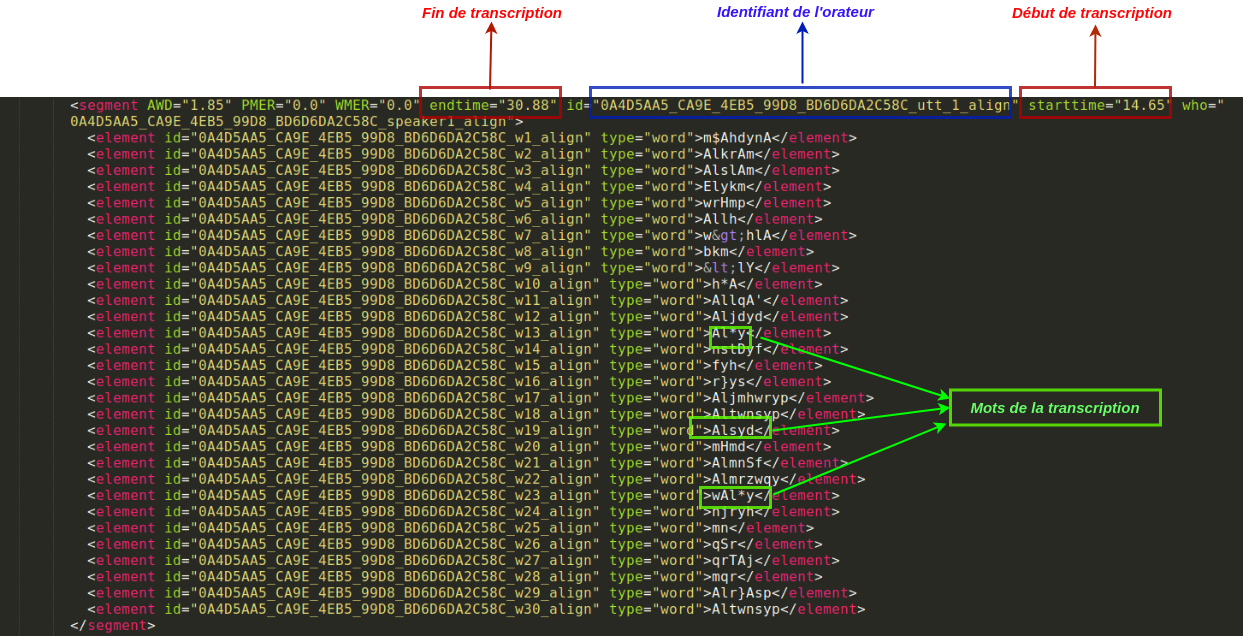
\includegraphics[width=400pt]{images/chap4/example_trans.png}
     \caption{Exemple de transcription dans un fichier XML du corpus élargi}
     \label{xml_exemple}
 \end{figure}
 
Nous implémentons donc l'algorithme que nous avons présenté dans la section \ref{collecte_donnees} en utilisant les méthodes de la bibliothèque Python "\textit{XML}" ainsi que les méthodes de la bibliothèque "\textit{Pydub}" pour effectuer le découpage des enregistrements audio selon les temps de début et fin d'enregistrement. 

 
\subsection{Conversion des fichiers audio et fichiers texte en dataset de dix heures}
Afin de rendre l'exploitation des données plus simple, mais surtout plus rapide, nous créons une classe que nous nommons \textit{"AudioInput"}. Cette classe aura pour but de contenir le spectrogramme de l'enregistrement, sa transcription, son chemin ainsi que sa durée. Ensuite, nous parcourons chaque couple de répertoires audio et fichier de transcriptions et appliquons les modifications liées aux caractères qui n'appartiennent pas à la table Buckwalter \cite{buckwalter} que nous avons citées dans la section \ref{trans_preprocessing}. Pour finir, nous définissons une limite de durée pour chaque dataset et générons des fichiers binaire de type \textit{Pickle} contenant une liste d'objets \textit{AudioInput} totalisant dix heures de dialogue.

Cette limite du nombre d'heures de dialogue pour chaque fichier Picke a pour but :
\begin{itemize}
    \item de simplifier l'upload des fichiers Pickle sur le cloud,
    \item d'éviter les dépassements de taille de mémoire vive lors de la génération de ces fichiers car nous libérons l'espace mémoire après avoir généré les dix heures,  
    \item de simplifier la séparation des datasets en données d'apprentissage et de test, et
    \item de faciliter la manipulation des datasets pour les 60 heures, 260 heures et 1200 heures d'apprentissage. \\
\end{itemize}

La génération de ce corpus est une opération qui a pris à la machine un total de quatre jours. Ce temps est due à la quantité de données à notre disposition, qui est de 118 GO, ainsi qu'à la durée de génération des spectrogrammes MFCC à l'aide de la bibliothèque \textit{Librosa}. Il est à noter que cette opération n'aurait pas pu se faire sans partitionnement des données à cause de la mémoire vive qui aurait été saturée. 

\subsection{Encodage des transcriptions}
Les réseaux de neurones ne traitent que les données numériques d'où la nécessité d'encoder les transcriptions sous forme de données numériques. Pour cela, deux approches s'offrent à nous : un encodage basé caractères et un encodage basé mots. Nous implémentons les algorithmes que nous avons présentés dans les sections \ref{character_based} et \ref{word_based} en utilisant la bibliothèque "\textit{NumPy}" pour les transcriptions.Après encodage, l'ensemble des transcriptions est sous forme d'une matrice "\textit{NumPy}" à 3 dimensions. La première dimension qui est un paramètre fixe représente le nombre de transcriptions; la deuxième dimension, variable quant-à elle, représente le nombre de mots par transcription; et, enfin, la troisième dimension qui est fixe, représente la taille de chaque mot selon l'encodage choisi.
 
\section{Implémentation des modèles}
Nous présentons dans cette section l'implémentation du modèle encodeur/décodeur, les différentes couches utilisées, l'environnement que nous avons mis en place pour l'apprentissage des modèles ainsi que l'envoi des données à l'algorithme d'apprentissage.

\subsection{Modèle Encodeur/Décodeur}
La base de notre système de reconnaissance de la parole est le modèle encodeur/décodeur. Pour l'implémenter, nous utilisons l'API fonctionnelle de \textit{Keras} \cite{functional_api} à travers la classe \textit{Model}. L'intérêt principal de cette classe est de créer des modèles pouvant avoir plusieurs inputs et plusieurs outputs. Dans le cas de notre système, nous avons l'entrée de l'encodeur ainsi que l'entrée du décodeur en input et la sortie, ou les sorties pour la reconnaissance basée mots, du décodeur en output du modèle.

\subsection{Couches utilisées}
Nous avons utilisé les couches nativement fournies par \textbf{Tensorflow} pour l'implémentation de nos modèles. Ces couches sont les suivantes : 

\begin{itemize}
    \item \textbf{Input} : couche permettant de définir une donnée comme étant une donnée de type input pour l'API fonctionnelle de Keras. Cette couche prend en entrée la dimension des données en entrée et est insérée avant de définir les couches de l'encodeur et du décodeur.\\
    
    \item \textbf{GRU} : nous nous sommes tournés vers l'utilisation des couches GRU. Celles-ci elles présentent des résultats très semblables aux couches LSTM mais sont plus rapides pour l'apprentissage et l'inférence. Ces couches sont utilisées pour l'encodeur et le décodeur afin de capturer et comprendre les données séquentielles. Une couche GRU prend en entrée un certain nombre de paramètres; le paramètre le plus important est sans doute "\textit{latent\_dim}" qui permet de spécifier la dimension de la représentation de l'entrée audio du modèle par l'encodeur. Il n'y a pas de mesure ou formule pour calculer la valeur idéale de ce paramètre; le choix de celui-ci est donc, à première vue, expérimental.\\
    
    \item \textbf{Bidirectional} : ce n'est pas une couche mais une enveloppe de couche qui prend en paramètre une couche récurrente et effectue l'apprentissage dans un sens des données puis dans le sens contraire.\\
    
    \item \textbf{Conv1D} : couche convolutionnelle à une dimension qui a pour paramètres "\textit{filters}" qui représente le nombre de filtres en sortie et le paramètre "\textit{kernel\_size}" qui, lui, représente la taille du masque de convolution.\\
    
    \item \textbf{MaxPooling1D} : prend en paramètre "\textit{pool\_size}" qui est la taille du vecteur qui se déplace dans le spectrogramme et retourne le maximum des valeurs contenues dans ce dernier.\\
    
    \item \textbf{Dense} : couche de sortie du modèle et a pour paramètres "\textit{units}" qui est la dimension de la donnée en sortie ainsi que "\textit{activation}" qui est la fonction d'activation de ce modèle. Pour notre problématique, nous utilisons la fonction d'activation "\textit{Softmax}". Cette fonction retourne des valeurs positives dans l'intervalle [0-1] ce qui, pour l'encodage One-Hot-Encoding, est nécessaire pour classifier les différents caractères.
\end{itemize}

\subsubsection{Fonction d'erreur}
Nous utilisons la fonction \textit{categorical\_crossentropy} pour le calcul de l'erreur lors de l'apprentissage. Cette fonction d'erreur est utilisée lorsqu'il y a plusieurs classes à prédire et que toutes les classes ont la valeur 0 à l'exception de la classe à prédire qui prend la valeur 1.

\subsubsection{Fonction d'apprentissage}\label{fonctionapp}
Une fonction d'apprentissage, ou optimizer en anglais, sert à minimiser la fonction d'erreur. Cette fonction est un hyper-paramètre qui peut être défini :
\begin{itemize}
    \item selon la problématique et les couches utilisées dans le modèle. Par exemple nous utilisons, en général, la fonction d'apprentissage \textit{RMSprop} lorsque nous utilisons des récurrentes \cite{keras_optimizers}, et
    \item selon les résultats de l'expérimentation. \\
\end{itemize}

Nous nous intéressons, pour commencer, à la fonction d'apprentissage \textit{RMSprop}, de la bibliothèque Keras \cite{keras_optimizers} car celle-ci est, en théorie, convenable à la nature de notre problème.

La seconde fonction que nous considérons est la fonction \textit{Adagrad} de Keras. \textit{Adagrad} a des taux d’apprentissage qui sont spécifiques à chaque paramètre du modèle et sont adaptés en fonction de la fréquence de mise à jour des poids des couches. Cette particularité fait de cette fonction un bon candidat pour l'apprentissage d'un système de reconnaissance de la parole où les poids sont très fréquemment mis à jour. 

Dans la suite de ce chapitre, nous expérimentons ces deux fonctions d'apprentissage pour définir celle qui répond le mieux à nos besoins. 

\subsection{Envoi des données pour l'apprentissage}
Afin qu'un modèle effectue son apprentissage, des données d'entraînement et de test sont nécessaires. Lorsque nous effectuons l'apprentissage sur des données de type séries temporelles, il n'est pas possible d'envoyer les données d'entrée et de sorties directement en paramètre à la méthode \textit{fit} de la classe \textit{Model} de Keras. Celle-ci doit connaître la dimension des entrées et, dans notre cas, les données n'ont pas le même nombre de timesteps.

Pour remédier à ce problème, nous utilisons la méthode \textit{fit\_generator} de la classe \textit{Model} de Keras qui prend comme paramètre d'entrée une méthode que nous implémentons pour envoyer les données ayant le même nombre de timesteps à la fois. L'algorithme \ref{Algo_timesteps} résume le fonctionnement de cette méthode. 

\begin{algorithm2e}[H]
\caption{Algorithme de sélection des données qui ont le même nombre de timesteps \label{Algo_timesteps}}
\SetAlgoLined
\SetKwInOut{Input}{Input}
\Input{liste\_audio : liste des fichiers Pickle contenant les enregistrement audio \\ liste\_transcriptions : liste des fichiers Pickle contenant les transcriptions \\ nombre\_données : nombre total de données}
 \While{Vrai}{
    \For{i $\in$ [0, nombre\_donnees]}{
    \tcc{Récuperer les pairs (clé-valeur) tel que la clé est un tuple (timestep\_audio, timestep\_transcription) et la valeur est une liste contenant les spectrogrammes et transcriptions de même timestep que la clé.}\\ 
            données $\gets$ pair(liste\_audio[i], liste\_transcriptions[i]) \\ 
            \For{(cle, valeur) $\in$ donnees}{
                sortie $\gets$ (cle, valeur) \\
                \For{element $\in$ sortie}{
                    \tcc{Envoyer les inputs et les outputs ayant les mêmes timesteps}\\
                    encoder\_x.ajouter(element[0][0]) \\
                    decoder\_x.ajouter(element[0][1]) \\
                    decoder\_y.ajouter(element[1]) \\
                }
            }
    }
    \tcc{Envoyer : traduite de "yield" qui envoie des données sans interrompre l'exécution de la fonction}
    envoyer [encoder\_x, decodeur\_x], decoder\_y \\
}
\end{algorithm2e}

Le second souci que nous avons rencontré est le grand volume de données envoyé en entrée du modèle ce qui donne des itérations d'une longue durée. Afin de remédier à cette complication, nous précisons la taille du batch\footnote{Batch : nombre de données à être envoyées pour chaque itération.} et calculons la probabilité d'envoyer un ensemble de données par rapport à un autre ensemble. Pour calculer ces probabilités nous avons défini la méthode \ref{prob_donnees} :

\begin{algorithm2e}[H]
\SetAlgoLined
\SetKwInOut{Input}{Input}
\SetKwInOut{Output}{Output}
\Input{batch\_size : nombre de données à envoyer dans un batch \\ 

dataset : Fichiers Pickle de spectrogrammes et transcriptions}
\Output{sortie : nombre d'instances à envoyer dans un batch\\}
\BlankLine
timesteps $\gets$ recuperer\_timesteps\_de\_meme\_taille(dataset)\\
taille\_valeurs $\gets$ somme(valeurs(timesteps)\\
probas $\gets$ initiliser\_dictionnaire() \\
\tcc{Récuperer le dictionnaire des probas qui contient les probabilités d'avoir envoyer la clé} 
\For{cle $\in$ timesteps}
    {proba[cle] $\gets$ taille(timesteps)/taille\_valeurs}
cles\_timesteps $\gets$ cles(timesteps)\\
nbr\_parititons $\gets$ taille\_valeurs/ batch\_size + 1 \\
\For{i $\in$ (0, nbr\_paritions)}\\
\tcc{Choisir au hasard un couple de timesteps selon la probabilité d'envoi de celui-ci} 
    r $\gets$ random() \\
    \For{cle $\in$ cles\_timesteps}
    {\If{r < proba[cle]}{sortie boucle} r $\gets$ r - proba[cle]}
    \tcc{Retourner toutes les données ayant les timesteps selon la taille du batch}
    sortie $\gets$ timesteps[cle] \\
    n\_batch\_size $\gets$ min(batch\_size, taille(sortie)) \\
    sortie $\gets$ random(sortie, n\_batch\_size) \\
    Retourner : sortie
 \caption{calcul de probabilité d'envoi d'un ensemble de données d'apprentissage \label{prob_donnees}}
\end{algorithm2e}

En sélectionnant les données à envoyer dans un batch aléatoirement, nous permettons au modèle d'effectuer un meilleur apprentissage. L'intuition derrière ce raisonnement est que lorsque les batchs sont envoyés au modèle dans le même ordre, celui-ci met à jour ses poids à la fin de l'itération en se basant toujours sur le même batch qu'il reçoit à la fin. Ainsi, envoyer les batchs de manière aléatoire permet au modèle de mettre à jour ses poids à la fin de l'itération sans effectuer son apprentissage sur les mêmes successions de données, améliorants ainsi les performances au test.

Nous passons à présent à la présentation de l'environnement utilisé ainsi que les différentes architectures avec leurs couches et leurs paramètres pour chaque corpus

\subsection{Environnement d'apprentissage}
Comme nous l'avons mentionné au début de ce chapitre, nous utilisons une machine Google Colaboratory \cite{colab} qui est basée sur le cloud. Nous utilisons principalement cette machine pour sa carte graphique ainsi que son nombre élevé de Cuda Cores\footnote{Cuda Core : Unité de calcul matricielle massivement parallèle dans les cartes graphiques}. Afin de profiter de la puissance de calcul de la carte graphique, nous utilisons la couche récurrente \textit{CuDNNGRU} à la place de \textit{GRU}. Les couches \textit{CuDNN} proposées par Keras permettent d'accélérer l'apprentissage des modèles à l'aide des GPU.

Google Colaboratory ne nous offre que la puissance de calcul graphique; l'apprentissage s'effectue de la même manière que sur une de nos machines. Afin de travailler à partir de Google Colaboratory, nous passons par les étapes suivantes : 
\begin{itemize}
    \item créer un Jupyter Notebook à l'aide d'un compte Google,
    \item cloner le code source du système de reconnaissance de la parole à partir du projet Github que nous avons créé,
    \item se connecter à une instance Google Drive pour en copier les jeux de données,
    \item lancer le script python d'apprentissage à partir du code source disponible sur Google Colaboratory. \\
\end{itemize}

La figure \ref{Colab} est un exemple d'environnement d'apprentissage avec Google Colaboratory.

\begin{figure}[H]
    \centering
    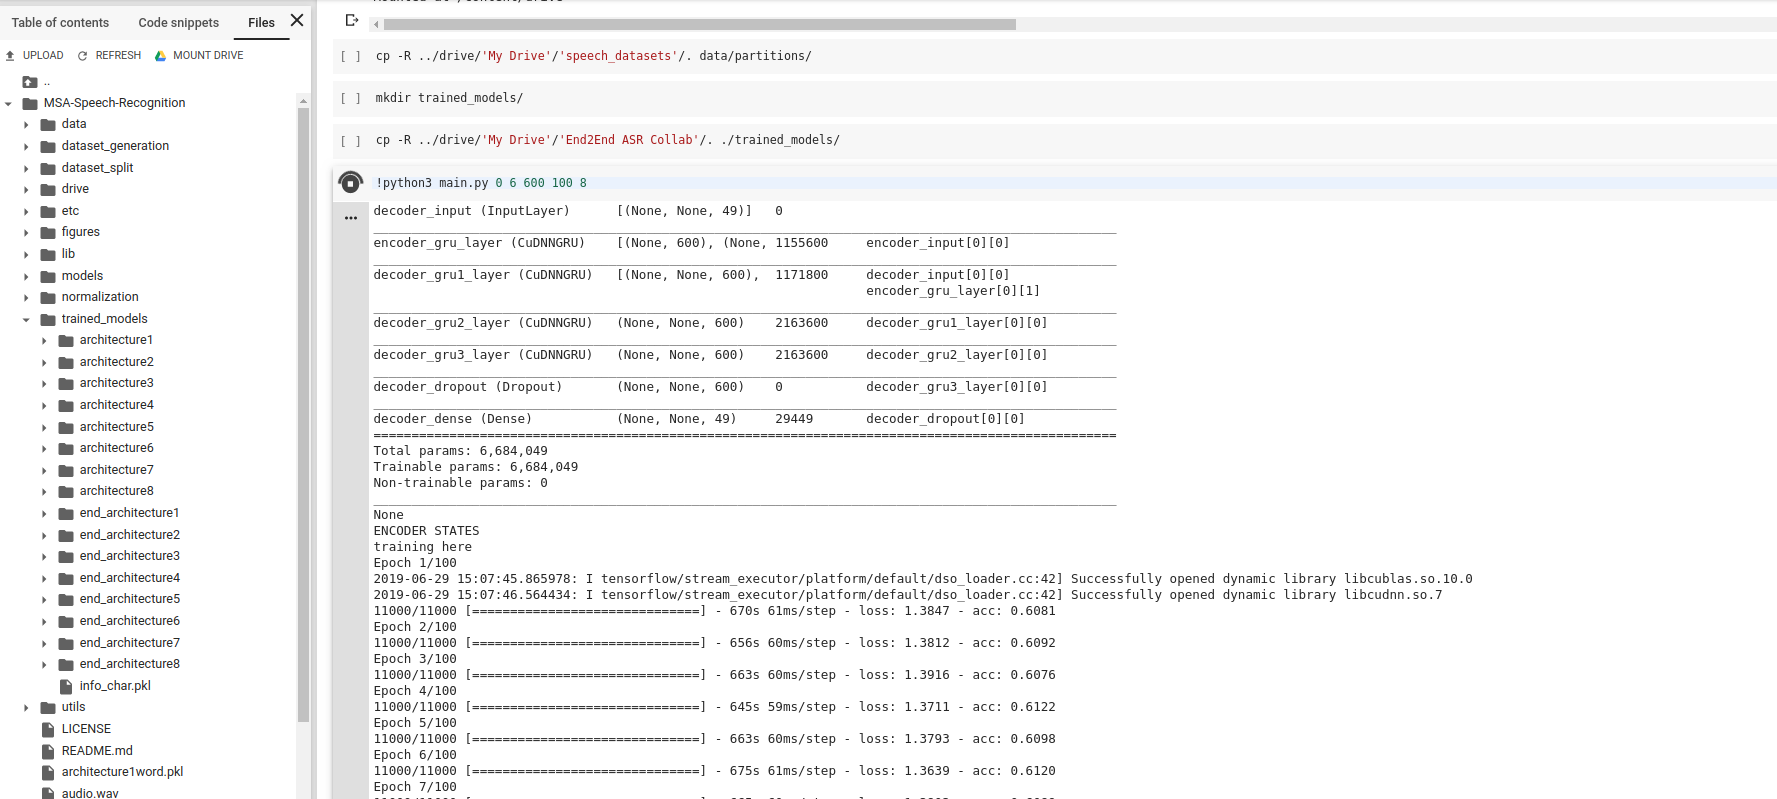
\includegraphics[width=450pt]{images/chap4/Collab.png}
    \caption{Exemple d'un environnement d'apprentissage avec Google Colaboratory}
    \label{Colab}
\end{figure}

Une difficulté que nous avons rencontrée est qu'une exécution à partir de Google Colaboratory ne dure que 12 heures et, une fois ce délai écoulé, toutes les données sur le disque sont effacées. Nous n'avions donc pas la possibilité d'enregistrer nos modèles pour poursuivre l'apprentissage. Afin de remédier à ce problème, nous sauvegardons le modèle ainsi que l'historique des courbes d'apprentissage sur Google Drive et ce, de manière automatique en implémentant la méthode \textit{on\_epoch\_end} dont l'appel s'effectue automatiquement à la fin de chaque itération.


\section{Apprentissage et discussion des résultats}
Nous passons à présent à l'apprentissage des modèles que nous avons définis dans la section \ref{apprentissage} de ce document. Pour la préparation des modèles et leurs apprentissages nous utilisons les couches que nous avons définies précédemment en variant les paramètres de celles-ci.

Pour l'apprentissage basé mots, chaque couche de sortie a sa propre exactitude et sa propre erreur. Pour une meilleure lecture des résultats nous calculons les moyennes des exactitudes et des erreurs sur les six premières couches de sortie car \textit{\%70} des mots du corpus ont une taille égale ou inférieure à six caractères, ce qui est assez représentatif. Nous avons choisi de calculer cette moyenne sur six caractères car seulement \textit{39\%} des mots ont cinq caractères ou moins. En plus de cela, au delà de six caractères les exactitudes sont très élevées car elles représentent les exactitudes des caractères de fin de mots. Prendre en compte les exactitudes de ces couches de sortie risquerait de biaiser la performance rapportée du système.

Nous présentons dans cette section les architectures pour chacun des modèles avec les meilleures performances au test sous forme de tableaux récapitulatifs et courbes de performances.

\subsection{Résultats d'apprentissage sur les différents corpus}
Nous présentons et discutons dans ce qui suit les résultats obtenus par les différentes architectures en nous basant sur les trois corpus suivants :
\begin{itemize}
    \item \textbf{Corpus d'essai} : ce corpus, que nous avons présenté dans la section \ref{corpus_essais}, est un corpus de six heures qui a pour but de tester le fonctionnement des différentes architectures. Nous effectuons l'apprentissage de cinq heures de dialogue et le test sur une heure.
    \item \textbf{60 heures de dialogue} : pour ce corpus nous effectuons l'apprentissage sur 52 heures de dialogue et le test sur huit heures. Ce corpus contient 35111 mots distincts, une taille de mots maximale de 15 caractères et un jeu de 42 caractères distincts.
    \item \textbf{260 heures de dialogue} : ce jeu de données contient 85532 mots distincts, une taille maximale de 16 caractères par mot pour un total de 49 caractères distincts. Nous divisons ces 260 heures de dialogue en 230 heures d'apprentissage et 30 heures de test.
\end{itemize}

\subsubsection{Apprentissage basé caractères}
Le tableau \ref{tableau1} résume les résultats de l'apprentissage en utilisant les couches unidirectionnelles avec les deux optimizers \textit{RMSprop} et \textit{Adagrad}. Le tableau \ref{tableau2} quant à lui résume les résultats obtenus avec les couches bidirectionnelles avec ces mêmes optimizers.

\begin{center}
\centering
    \begin{table}[H]
    \caption{Performances de l'apprentissage basé caractères avec couches unidirectionnelles}
    \label{tableau1}
    \resizebox{\textwidth}{!} & \makecell{71\%} & \makecell{75\%}\\
         \cline{6-9}
          &  &  &  &  & \makecell{Adagrad} & \makecell{31\%} & \makecell{69\%} & \makecell{88\%}\\
         \hline
         
          \multirow{2}*\makecell{six heures} & \multirow{2}*\makecell{2 Conv1D} & \multirow{2}*\makecell{1 GRU} &\multirow{2}*\makecell{2 GRU}  &\multirow{2}*\makecell{400} & \makecell{RMSprop} & \makecell{27\%} & \makecell{73\%}& \makecell{87\%}\\
         \cline{6-9}
          &  &  &  & & \makecell{Adagrad} & \makecell{32\%} & \makecell{68\%}& \makecell{87\%}\\
         \hline

         \multirow{2}*\makecell{60 heures} & \multirow{2}*\makecell{-} & \multirow{2}*\makecell{1 GRU} &\multirow{2}*\makecell{2 GRU}  & \multirow{2}*\makecell{500} & \makecell{RMSprop} & \makecell{42\%} &  \makecell{58\%}& \makecell{72\%}\\
         \cline{6-9}
          &  &  &  &  & \makecell{Adagrad} & \makecell{42\%} &   \makecell{58\%}& \makecell{72\%}\\
         \hline
          \multirow{2}*\makecell{60 heures} & \multirow{2}*\makecell{2 Conv1D} & \multirow{2}*\makecell{1 GRU} &\multirow{2}*\makecell{2 GRU}  & \multirow{2}*\makecell{400} & \makecell{RMSprop} & \makecell{40\%} & \makecell{70\%}& \makecell{73\%}\\
         \cline{6-9}
          &  &  & &  & \makecell{Adagrad} & \makecell{43\%} & \makecell{57\%}& \makecell{68\%}\\
         \hline
         
         \multirow{2}*\makecell{260 heures} & \multirow{2}*\makecell{-} & \multirow{2}*\makecell{1 GRU} &\multirow{2}*\makecell{3 GRU} &\multirow{2}*\makecell{550} & \makecell{RMSprop} & \makecell{51\%} & \makecell{49\%}& \makecell{54\%}\\
         \cline{6-9}
          &  &  & & & \makecell{Adagrad} & \makecell{68\%} & \makecell{32\%}& \makecell{41\%}\\
         \hline

         \multirow{2}*\makecell{260 heures} & \multirow{2}*\makecell{3 Conv1D} & \multirow{2}*\makecell{1 GRU} &\multirow{2}*\makecell{3 GRU} &\multirow{2}*\makecell{500} & \makecell{RMSprop} & \makecell{49\%} & \makecell{51\%}& \makecell{53\%}\\
         \cline{6-9}
          &  &  & & & \makecell{Adagrad} & \makecell{71\%} & \makecell{29\%}& \makecell{38\%}\\
         \hline
                
    \end{tabular}}
    \end{table}
\end{center}
\FloatBarrier

\begin{center}
\centering
    \begin{table}[H]
    \caption{Performances de l'apprentissage basé caractères avec couches bidirectionnelles}
    \label{tableau2}
    \resizebox{\textwidth}{!} & \makecell{74\%}& \makecell{89\%}\\
         \cline{6-9}
         
         \multirow{2}*\makecell{six heures} & \multirow{2}*\makecell{-} & \multirow{2}*\makecell{1 GRU} &\multirow{2}*\makecell{2 GRU}  &\multirow{2}*\makecell{500} & \makecell{Adagrad} &\makecell{26\%} & \makecell{74\%}& \makecell{91\%}\\
         \hline
         
          &  &  &  & & \makecell{RMSprop} & \makecell{22\%} & \makecell{78\%}& \makecell{89\%}\\
         \cline{6-9}
        
         \multirow{2}*\makecell{six heures} & \multirow{2}*\makecell{2 Conv1D} & \multirow{2}*\makecell{1 GRU} &\multirow{2}*\makecell{2 GRU}  &\multirow{2}*\makecell{400} & \makecell{Adagrad} & \makecell{25\%} & \makecell{75\%}& \makecell{89\%}\\
         \hline
         
          &  &  & & & \makecell{RMSprop} & \makecell{33\%} & \makecell{67\%}& \makecell{80\%}\\
         \cline{6-9}
         
         \multirow{2}*\makecell{60 heures} & \multirow{2}*\makecell{-} & \multirow{2}*\makecell{1 GRU} &\multirow{2}*\makecell{2 GRU} &\multirow{2}*\makecell{500} & \makecell{Adagrad} & \makecell{36\%} & \makecell{64\%}& \makecell{73\%}\\
         \hline
          &  &  & & & \makecell{RMSprop} & \makecell{34\%} & \makecell{77\%}& \makecell{79\%}\\
         \cline{6-9}
         
         \multirow{2}*\makecell{60 heures} & \multirow{2}*\makecell{2 Conv1D} & \multirow{2}*\makecell{1 GRU} &\multirow{2}*\makecell{2 GRU} &\multirow{2}*\makecell{400} & \makecell{Adagrad} & \makecell{37\%} & \makecell{73\%}& \makecell{70\%}\\
         \hline
           &  &  & &  & \makecell{RMSprop} & \makecell{49\%} & \makecell{51\%}& \makecell{54\%}\\
         \cline{6-9}
         
          \multirow{2}*\makecell{260 heures} & \multirow{2}*\makecell{-} & \multirow{2}*\makecell{1 GRU} &\multirow{2}*\makecell{3 GRU} & \multirow{2}*\makecell{550} & \makecell{Adagrad} & \makecell{64\%} & \makecell{36\%}& \makecell{43\%}\\
         \hline 
           &  &  &  &  & \makecell{RMSprop} & \makecell{49\%} & \makecell{51\%}& \makecell{56\%}\\
         \cline{6-9}

          \multirow{2}*\makecell{260 heures} & \multirow{2}*\makecell{3 Conv1D} & \multirow{2}*\makecell{1 GRU} &\multirow{2}*\makecell{3 GRU} & \multirow{2}*\makecell{500} & \makecell{Adagrad} & \makecell{68\%} & \makecell{32\%}& \makecell{41\%}\\
          \hline
    \end{tabular}}
    \end{table}
\end{center}
\FloatBarrier

\textbf{Discussion des résultats :} Nous remarquons tout de suite une grande différence entre les résultats obtenus pour chaque optimizer. La fonction \textit{Adagrad} présente des résultats nettement meilleurs que \textit{RMSprop}. Nous nous intéressons donc aux résultats obtenus avec l'utilisation de \textit{Adagrad}. Nous discutons ces résultats pour chaque corpus afin d'étudier l'évolution des performances des modèles avec l'augmentation du volume de données. Cette étude nous permettra de choisir, sur la base des résultats obtenus, le modèle adéquat pour l'apprentissage sur les 1200 heures de dialogue.

\begin{itemize}
    \item \textbf{Corpus d'essai (six heures de dialogue)} : nous ne pouvons donner une interprétation digne d'intérêt aux résultats obtenus à partir du corpus d'essai. En effet, pour une problématique aussi complexe que la reconnaissance de la parole en utilisant un modèle End-To-End, cinq heures de dialogue ne sont pas représentatives provoquent clairement un sous apprentissage. Ce corpus a été utilisé uniquement dans le but de tester le bon fonctionnement de nos modèles. Nous passons à l'apprentissage sur 60 heures de dialogue pour obtenir des résultats plus représentatifs. \\
    
    \item \textbf{60 heures de dialogue :} la première chose que nous notons est une hausse des résultats d'apprentissage par rapport au corpus d'essai. Lors de cet apprentissage, l'exactitude de l'apprentissage pour chacun des modèles à atteint les 99\%. Cependant comme le montre le tableau ci-dessus, les exactitudes de test ne dépassent pas les 43\% ce qui est un signe de sur-apprentissage. Nous expliquons cela par le faible nombre de données d'apprentissage pour une problématique aussi complexe que la reconnaissance de la parole. \\
    
    \item \textbf{260 heures de dialogue :} avec 260 heures de dialogue, nous notons une nette amélioration des résultats d'apprentissage en comparaison avec les 60 heures. L'augmentation du volume de données a permis de minimiser le sur-apprentissage. En effet, les exactitudes d'apprentissage sont de 75\% en moyenne. Nous remarquons également que le modèle à couches convolutionnelles a présenté les meilleurs résultats. Ceci est dû au traitement qu'effectuent les couches convolutionnelles sur les spectrogrammes avant que ceux-ci soient envoyés à l'encodeur. Notons cependant, que les modèles à couches bidirectionnelles ont présenté des résultats moin satisfaisants que les autres modèles. Ceci est dû à la quantité de données encore insuffisante ainsi qu'au temps que nous avons accordé aux apprentissages. Les modèles à couches bidirectionnelles prennent beaucoup plus de temps lors de l'apprentissage en comparaison aux autres modèles. Nous ne tentons pas d'aller plus loin dans l'apprentissage de ces modèles au vu de la limite de temps imparti pour la réalisation de ce projet. 
\end{itemize}

\subsubsection{Apprentissage basé mots}
Nous adoptons donc pour cet apprentissage l'architecture à plusieurs couches de sortie où chaque couche \textit{n} doit pouvoir reconnaître le \textit{nième} caractère d'un mot. Ce nombre de couches est égal au nombre maximum de caractères par mot. Au vu de la supériorité de la fonction \textit{Adagrad} par rapport à \textit{RMSprop}, pour notre problématique du moins, nous effectuons nos apprentissages avec \textit{Adagrad} uniquement. 

Comme pour l'apprentissage basé caractères, le tableau \ref{tableau3} concerne les couches unidirectionnelles quant au tableau \ref{tableau4}, il concerne les couches bidirectionnelles. Les résultats d'apprentissage sont les suivants.

\begin{center}
\centering
    \begin{table}[H]
    \caption{Performances de l'apprentissage basé mots avec couches unidirectionnelles}
    \label{tableau3}
    \resizebox{\textwidth}{!} & \makecell{78\%} & \makecell{82\%}\\
         \cline{2-8}
         
          & \makecell{2 Conv1D} & \makecell{1 GRU} &\makecell{2 GRU}  &\makecell{400} & \makecell{17\%} & \makecell{79\%}& \makecell{83\%}\\
         \hline
         
         \multirow{2}*\makecell{60 heures} & \makecell{-} & \makecell{1 GRU} &\makecell{2 GRU}  & \makecell{500} & \makecell{29\%} & \makecell{66\%}& \makecell{71\%}\\
         \cline{2-8}
         
           & \makecell{2 Conv1D} & \makecell{1 GRU} &\makecell{2 GRU}  & \makecell{400} & \makecell{31\%} & \makecell{67\%}& \makecell{69\%}\\
         \hline
         
         \multirow{2}*\makecell{260 heures} & \makecell{-} & \makecell{1 GRU} &\makecell{3 GRU} &\makecell{550} & \makecell{56\%} & \makecell{39\%}& \makecell{44\%}\\
         \cline{2-8}
          & \makecell{3 Conv1D} & \makecell{1 GRU} &\makecell{3 GRU} &\makecell{500} & \makecell{58\%} & \makecell{36\%}& \makecell{42\%}\\
         \hline
        
    \end{tabular}}
    \end{table}
\end{center}
\FloatBarrier
\begin{center}
\centering
    \begin{table}[H]
    \caption{Performances de l'apprentissage basé mots avec couches bidirectionnelles}
    \label{tableau4}
    \resizebox{\textwidth}{!} & \makecell{83\%}& \makecell{88\%}\\
         \cline{2-8}
         
         
          & \makecell{2 Conv1D} & \makecell{1 GRU} &\makecell{2 GRU}  &\makecell{400} & \makecell{14\%} & \makecell{83\%}& \makecell{86\%}\\
         \hline
         
         
         \multirow{2}*\makecell{60 heures} & \makecell{-} & \makecell{1 GRU} &\makecell{2 GRU} &\makecell{500} & \makecell{25\%} & \makecell{64\%}& \makecell{75\%}\\
         \cline{2-8}
          & \makecell{2 Conv1D} & \makecell{1 GRU} &\makecell{2 GRU} &\makecell{400} & \makecell{27\%} & \makecell{71\%}& \makecell{73\%}\\
         \hline
         
                 
          \multirow{2}*\makecell{260 heures} & \makecell{-} & \makecell{1 GRU} &\makecell{3 GRU} & \makecell{550} & \makecell{51\%} & \makecell{44\%}& \makecell{49\%}\\
         \cline{2-8} 
            & \makecell{3 Conv1D} & \makecell{1 GRU} &\makecell{3 GRU} & \makecell{500} & \makecell{55\%} & \makecell{39\%}& \makecell{45\%}\\
         \hline 
        
    \end{tabular}}
    \end{table}
\end{center}
\FloatBarrier

\textbf{Discussion des résultats} : Ici encore, nous discutons les résultats obtenus par les différents corpus à l'exception du corpus d'essai. 
\begin{itemize}

    \item \textbf{60 heures de dialogue} : nous remarquons une légère amélioration de la performance par rapport au corpus d'essai. Comme pour la reconnaissance basée caractères, l'exactitude d'apprentissage atteint les 99\% pour chaque modèle. Nous nous retrouvons donc dans une situation de sur-apprentissage. Nous justifions ce résultat par le nombre insuffisant de données d'apprentissage. En effet, pour l'apprentissage basé mots, le modèle a \textit{n} couches de sortie comme nous l'avons expliqué au début de cette section ce qui rend l'apprentissage sensiblement plus complexe. Nous ne pouvons espérer de bons résultats sans augmenter le volume de données. \\ 
    
    \item \textbf{260 heures de dialogue} : comme nous nous y attendions, nous notons une amélioration des performances qui est liée à l'augmentation du volume de données. Nous remarquons que le modèle à couches convolutionnelles a présenté les meilleurs résultats d'apprentissage même si l'exactitude n'est que de 58\% au test. Nous notons également un rapprochement entre l'exactitude d'apprentissage et de test minimisant ainsi le sur-apprentissage. Nous pensons que pour la reconnaissance basée mots, qui est de loin plus complexe que la reconnaissance basée caractères, un plus grand nombre de données est nécessaire. Nous étayons ce raisonnement par l'évolution de la performance lorsque nous sommes passé de 60 heures à 260 heures de dialogue. \\
\end{itemize}

Nous ne prenons pas la risque de lancer un apprentissage basé mots sur les 1200 heures de dialogue. Même si nous pensons que le modèle va enregistrer une performance nettement meilleure, nous ne pourrons en être sûrs sans expérimentation. 

L'apprentissage sur le corpus élargi, après un bref test, prend entre 15 et 20 minutes par itération d'où l'impossibilité de lancer un apprentissage sans être sûr de la performance que peut apporter le modèle. Nous ne savons pas si cette quantité de données suffirait au modèle. Il nous semble donc plus adéquat de lancer un apprentissage basé caractères en introduisant un modèle de langage pour améliorer encore plus la performance du modèle.

\subsection{Apprentissage sur le corpus élargi}
\subsubsection{Choix du modèle}
Notre choix quant au modèle que nous utilisons pour le développement de \textit{ASeR-System} s'est porté sur le modèle à couches convolutionnelles basé reconnaissance de caractères. Ce choix se justifie par les résultats prometteurs qu'a obtenu le modèle à couches convolutionnelles comparé aux autres modèles. Nous n'excluons pas la possibilité que les architectures à couches bidirectionnelles puissent présenter des résultats équivalents ou légèrement supérieurs aux résultats du modèle CNN mais nous ne pouvons déterminer à partir de quel volume de données ces modèles pourraient prendre le dessus sur le modèle CNN. Nous sommes également limité par la contrainte de temps car les modèles bidirectionnelles prennent plusieurs semaines d'apprentissage \cite{e2e4}.


\subsubsection{Apprentissage}
Après le pré-traitement des données, nous nous sommes retrouvés avec 860 heures de dialogue que nous avons divisées en 780 heures pour l'apprentissage et 80 heures pour le test. Ce corpus se compose de 153500 mots distincts et 49 caractères distincts. Le tableau \ref{perfappelargi} détaille l'architecture que nous avons mise en place. Il est à noter que les résultats ne sont pas finaux et que l'apprentissage est toujours en cours.

\begin{center}
\centering
    \begin{table}[H]
    \caption{Performance apprentissage modèle CNN sur le corpus élargi}
    \resizebox{\textwidth}{!} & \makecell{26\%} &\makecell{17\%}\\
         \hline
    \end{tabular}
    \label{perfappelargi}
    }
    \end{table}
\end{center}
\FloatBarrier

Les résultats obtenu avec le corpus élargi sont prometteurs. Nous estimons qu'en ajoutant du temps à l'apprentissage du modèle, celui-ci pourrait achever une meilleure performance. Augmenter le volume des données est également un garant de l'amélioration de la performance de ce modèle et est tout l'intérêt de l'utilisation de l'approche End-To-End.

\section{Environnement de développement pour la reconnaissance de la parole}
Nous présentons dans cette section l'implémentation de l'environnement de développement pour la reconnaissance de la parole ainsi que l'ensemble des paramétrages que nous avons mis en place. Pour le développement de cet environnement, nous nous sommes inspirés de la convention PEP8 en matière d'organisation pour simplifier à tout utilisateur l'intégration de nos modèles ou encore l'apprentissage de nouveaux modèles. Le schéma \ref{env_dev} résume l'organisation de l'environnement :

 \begin{figure}[H]
     \centering
     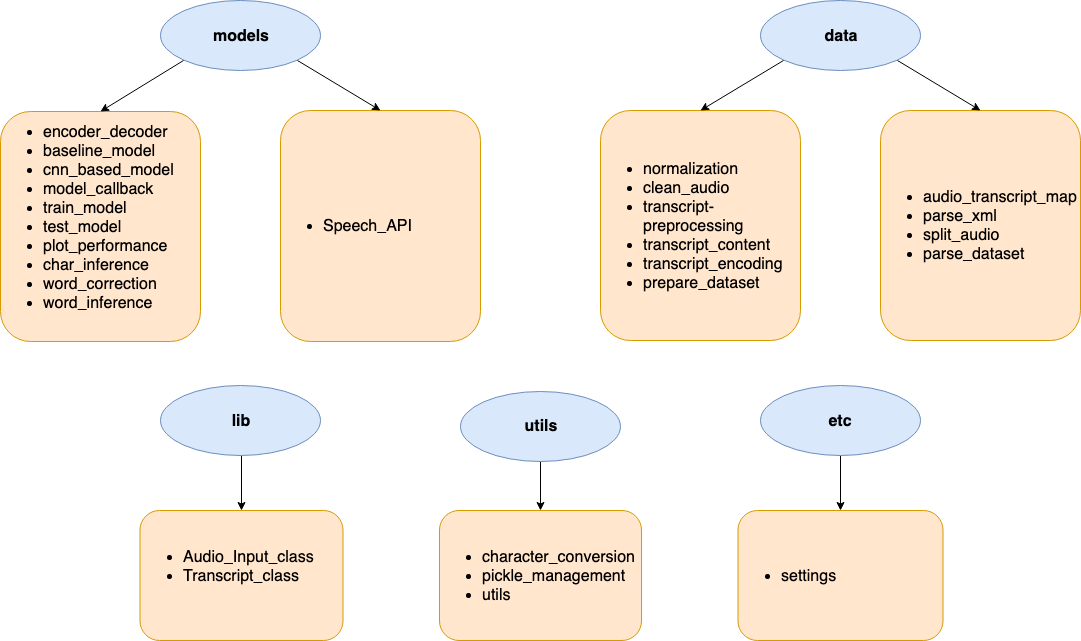
\includegraphics[height=275pt,width=400pt]{images/chap4/engine_packages.png}
     \caption{Disposition des packages de l'environnement de reconnaissance de la parole}
     \label{env_dev}
 \end{figure}

Nous avons implémenté l'environnement de développement de telle sorte à permettre à l'utilisateur d'utiliser chaque module indépendamment des autres modules. les modules sont les suivants : 
\begin{itemize}
    \item \textbf{models : } Ce module se divise en deux modules :
    \begin{enumerate}
        \item \textbf{Speech\_API} : module contenant un système de reconnaissance de la parole End-To-End prêt à intégrer à n'importe quelle application d'un simple appel de fonction.
        \item \textbf{Apprentissage :} Permettant d'effectuer l'apprentissage d'un modèle en second lieu. L'utilisateur a la liberté de modifier les couches utilisées pour l'apprentissage. Il est cependant à noter que tout changement dans les couches de l'architecture implique un changement au niveau de l'inférence. 
    \end{enumerate}
    \item \textbf{data :} Ce module se décompose à son tour en deux modules : 
        \begin{enumerate}
            \item \textbf{Génération de dataset :} Module semi-automatisé permettant de générer à partir d'enregistrements audio et transcriptions en format texte des fichiers Pickle, selon un nombre d'heures que peut définir l'utilisateur s'il le souhaite, associant à chaque enregistrement audio un spectrogramme MFCC ainsi que sa transcription. Ce module est semi-automatisé car les jeux de données ne sont pas toujours idéalement présentés (comme ce fut le cas pour le QCRI Speech Dataset).
            \item \textbf{Pré-traitement des données :} Ce module permet un certain nombre d'opérations sur les données tel que la normalisation des spectrogrammes, la suppression des enregistrements de mauvaise taille (d'une durée trop courte ou trop longue) ainsi que plusieurs types d'encodages des transcriptions comme nous l'avons présenté dans la section \ref{trans_preprocessing}. 
        \end{enumerate}
    \item \textbf{lib :} Module contenant les différentes classes utilisées.
    \item \textbf{utils :} Contenant différentes méthodes pour la gestion des répertoires et fichiers, conversion des caractères de Buckwalter vers l'arabe et vice versa, conversion binaire et bien d'autres.
    \item \textbf{etc :} Contenant les chemins relatifs et variables globales utilisées pour le pré-traitement et l'apprentissage.\\
\end{itemize}

Nous avons également mis en place une documentation détaillée concernant le fonctionnement de l'environnement de développement qui est disponible sur Github avec le système. Cette documentation est également disponible dans l'annexe de ce mémoire.

\section{Intégration du Système de questions-réponses}
Après avoir développé \textit{ASeR-System}, il est temps de le tester sur un vrai domaine d'application. Comme nous l'avons mentionné dans la section \ref{QASChap3}, nous avons choisi le domaine des systèmes de questions-réponses et plus particulièrement \textit{AFaQ-System}. \\

\textit{AFaQ-System} est basé sur un ensemble des paramètres que nous avons la possibilité de modifier pour effectuer différents tests. Ces paramètres sont les suivants : 
\begin{itemize}
    \item \textbf{--Mode :} définit le mode de recherche. Deux possibilités s'offrent à nous : le mode "Online" pour la recherche de réponses via le Web et le mode "Offline" dans le cadre de l'utilisation d'un corpus local.
    \item \textbf{--Source :} une chaîne de caractères précisant le chemin vers le corpus.
    \item \textbf{--Seuil :} représente le seuil de sélection des phrases pertinentes.
    \item \textbf{--SentenceSelection :} définit le nom du modèle à utiliser dans la phase de sélection des phrases.
    \item \textbf{--Model\_Path :} chaîne de caractères pour le chemin vers le modèle.
    \item \textbf{--NbrPassage :} le nombre des phrases à  sélectionner. \\
\end{itemize}
 
Dans notre cas, nous gardons les valeurs par défaut pour tous les paramètres cités sauf pour le \textbf{--mode} que nous mettons à Online pour ne pas être restreints à un corpus local. 

L'intégration \textit{AFaQ-System} avec \textit{ASeR-System} fut très simple, il nous a suffit d'appeler la fonction principale \textit{ArabicQuestionAnsweringSystem} du système de quesions-réponses en lui donnant en entrée la question qui représente la transcription de notre audio pour avoir la réponse en format texte.

\section{Application de ASeR-System sur un système de questions-réponses}
Afin de tester le bon fonctionnement de notre système de reconnaissance de la parole, nous avons développé une application Desktop avec la bibliothèque \textit{PyQT}. Cette application a pour objectif : 
\begin{itemize}
    \item d'effectuer un enregistrement sonore,
    \item d'utiliser la Speech\_API de \textit{ASeR-System} afin de générer la transcription de l'enregistrement sonore, 
    \item de trouver une réponse à la demande de l'enregistrement sonore en utilisant \textit{AFaQ-system}, et
    \item permettre à l'utilisateur de contribuer au projet en enregistrant un audio correspondant à une transcription afin d'augmenter la taille du corpus et ainsi, améliorer la performance de AeER-System.\\
\end{itemize}

Comme cette application est à but de test uniquement, nous avons développé une interface graphique simple et intuitive  permettant de réaliser les tâches ci-dessus. La figure \ref{main_window} présente la fenêtre principale de l'interface :

\begin{figure}[H]
     \centering
     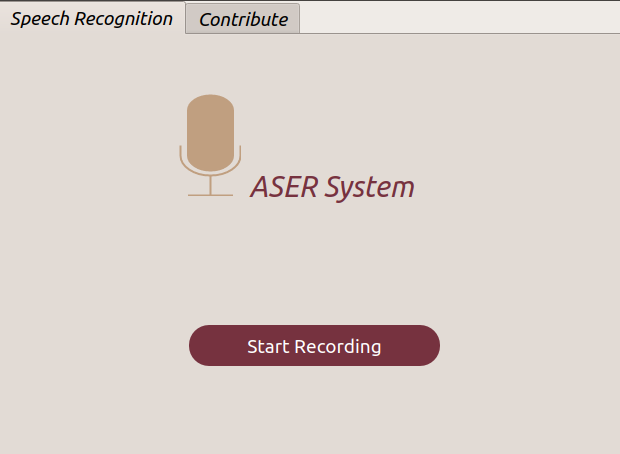
\includegraphics[height=250pt,width=430pt]{images/chap4/main_window.png}
     \caption{Fenêtre principale de l'application}
     \label{main_window}
 \end{figure}
 
 Ensuite, après avoir enregistré une question, \textit{ASeR-System} effectue la reconnaissance du dialogue contenu dans l'enregistrement et génère une transcription.  
 
\begin{figure}[H]
     \centering
     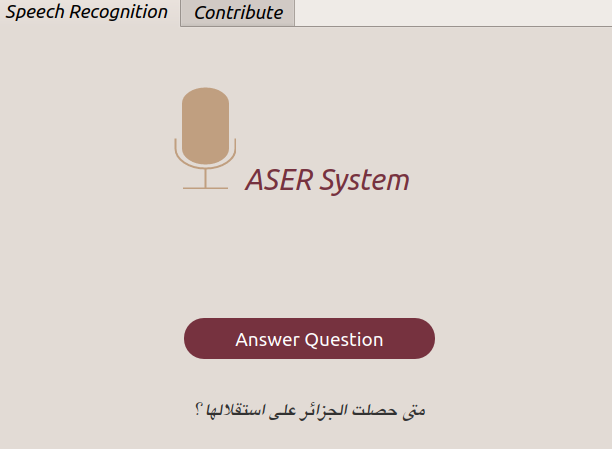
\includegraphics[height=250pt,width=430pt]{images/chap4/transcript_decoded.png}
     \caption{Affichage de la transcription}
     \label{}
 \end{figure}
 
Une fois la reconnaissance effectuée, l'utilisateur peut décider d'afficher une réponse à sa question et c'est là où nous faisons appel à \textit{AFaQ-System} pour trouver une réponse à cette question.
 
\begin{figure}[H]
     \centering
     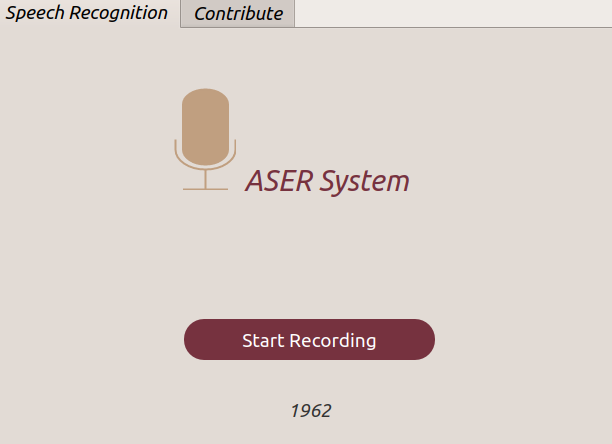
\includegraphics[height=250pt,width=430pt]{images/chap4/answer.png}
     \caption{Réponse à la question}
     \label{}
 \end{figure}
 
Nous avons également introduit un onglet contribution. Cette partie de l'application nous aidera à améliorer la performance de \textit{ASeR-System}. Nous générons aléatoirement des transcriptions à l'utilisateur pour que celui-ci enregistre un audio correspondant à ces transcriptions.

\begin{figure}[H]
     \centering
     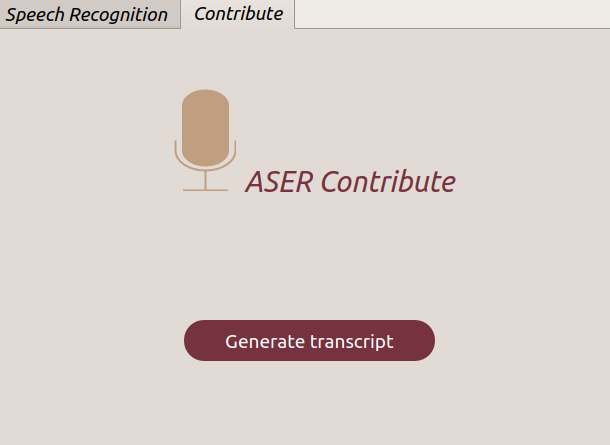
\includegraphics[height=250pt,width=430pt]{images/chap4/main_contribute.png}
     \caption{Onglet contribution de l'application}
     \label{}
 \end{figure}

Nous conservons ces enregistrements dans une base de données MySQL pour une utilisation future. 
 
 \begin{figure}[H]
     \centering
     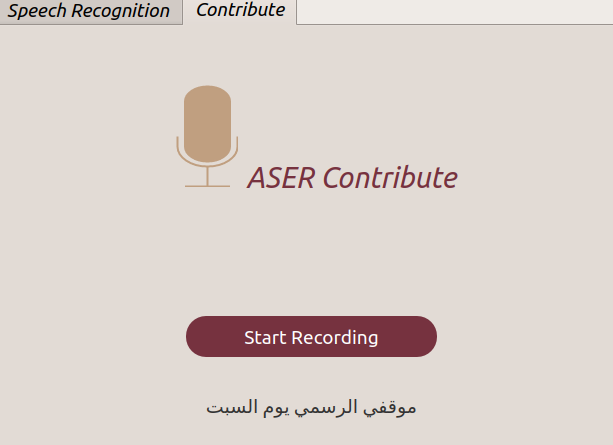
\includegraphics[height=250pt,width=430pt]{images/chap4/record_contribute.png}
     \caption{Génération d'une transcription pour la contribution}
     \label{}
 \end{figure}
 
Cette application est un exemple concret de l'utilisation du système de reconnaissance de la parole pour n'importe quel cas de figure tel qu'un système de questions-réponses.

\section{Conclusion}
À travers ce chapitre, nous avons présenté l'implémentation des différents modules de \textit{ASeR-System} en passant par l'environnement de travail, les différentes librairies utilisées mais aussi la génération des données d'apprentissage, la normalisation et la préparation des différents modèles. Nous avons également discuté les résultats d'apprentissage obtenus par les différents modèles et particulièrement le modèle final que nous avons choisi pour notre système de reconnaissance de la parole.

Nous avons conclu avec la présentation de l'application que nous avons réalisée pour tester \textit{ASeR-System} sur un système de questions-réponses. Cette application montre bien que notre environnement de développement permet de créer des systèmes de reconnaissance de la parole qui peuvent être utilisés dans tout type d'application de traitement automatique du langage naturel. 

\chapter*{Conclusion générale et perspectives} % Ne numérote pas le chapitre
\addcontentsline{toc}{chapter}{Conclusion générale et perspectives} % Référence l'introduction dans la table des matières
\chaptermark{Conclusion générale et perspectives}
La motivation principale de ce travail a été de créer un système de reconnaissance de la parole pour la langue arabe en se basant sur plusieurs représentations des données et plusieurs architectures de modèles. Ce système a été par la suite utilisé dans une application avec un système de questions-réponses. Nous avons également créé un environnement de développement en offrant une base solide pour le pré-traitement des données et l'apprentissage des modèles permettant ainsi aux chercheurs de pousser la recherche dans le domaine.

La première étape de ce travail a été l'étude du fonctionnement général des systèmes de reconnaissance de la parole en mettant en avant les différentes approches pour développer de tels systèmes. Ensuite, nous avons introduit les systèmes de questions-réponses, leurs architectures et leur fonctionnement car ces systèmes sont un excellent cas d'application pour la reconnaissance de la parole, \ie sur lesquels une couche de reconnaissance de la parole peut être placée. 

Une grande partie de notre travail fut l'étude de l'état de l'art en ce qui concerne les systèmes de reconnaissance de la parole. Cette étude a permis d'identifier les travaux les plus prometteurs en la matière et, plus particulièrement, les systèmes End-To-End qui sont encore récents et en pleine ascension. Nous avons également étudié et introduit les techniques avancées d'apprentissage profond qui sont utilisées dans ces systèmes. 

Vint ensuite la conception de \textit{ASeR-System}, notre système de reconnaissance de la parole pour la langue arabe avec les étapes de collecte et de nettoyage des données. Par la suite, nous avons approfondi le pré-traitement de ces données en proposant une représentation basée caractères et une représentation basée mots avec plusieurs encodages. Pour finir, nous avons conçu non pas une, mais quatre architectures de modèles que nous proposons dans notre environnement de développement.

Après l'étape de conception, ce fut le tour de l'implémentation de \textit{ASeR-System} en passant par le pré-traitement des données, l'apprentissage des modèles sur plusieurs tailles de corpus, l'étude et la discussion des résultats obtenus. Nous l'avons testé sur un système de questions-réponses à travers une application développée à cet effet. Nous avons également implémenté les différents modules de notre environnement de développement de systèmes de reconnaissance de la parole. 

% qui permet d'intégrer \textit{ASeR-System} et de l'améliorer. En plus de cela, cet environnement permet de créer de nouveaux systèmes de reconnaissance de la parole en utilisant des architectures différentes ou encore, des jeux de données différents.

Les principaux freins à ce projet furent le nombre limité, comparé à d'autres travaux, de données à notre disposition, le manque de moyens en terme de RAM et de GPU ainsi que le manque de temps pour l'apprentissage profond qui s'avère très complexe et nécessite des semaines d'apprentissage sur les données. Nous avons néanmoins mis en place tous les outils nécessaires en terme de modèles et de gestion dynamique de la mémoire pour permettre d'améliorer ou de recréer les modèles déjà existants en utilisant d'autres jeux de données plus élaborés. 

Il est important de noter que notre travail s'inscrit dans le cadre d'un projet de recherche et reste donc perfectible. En effet, plusieurs points peuvent être améliorés pour avoir des systèmes de reconnaissance de la parole arabe aussi performants que possible. Les perspectives de ce projet sont, par ordre décroissant d'importance, les suivantes : 
\begin{itemize}
    \item apprentissage des modèles et particulièrement les modèles bidirectionnels pour une période de temps supplémentaire;
    \item envoi de l'enregistrement audio sous forme de plusieurs découpes d'enregistrements pour afficher à l'utilisateur les résultats de la reconnaissance au fur et à mesure de l'enregistrement;
    \item ajout du mécanisme d'attention;
    \item développement et traitement d'un corpus de plusieurs milliers d'heures de dialogue pour parfaire l'apprentissage des modèles;
    \item traitement des noms propres dans les corpus qui peuvent être écrits dans un alphabet qui n'est pas l'alphabet Buckwalter comme ce fut le cas avec le QCRI Corpus; 
    \item génération automatisée de corpus d'enregistrements audio et de transcriptions quelle que soit leur présentation comme fonctionnalité de l'environnement de développement; et
    \item implémentation d'une fonction d'apprentissage PSO (particle Swarm Optimization) basée sur le principe d'intelligence en essaim. Le but de cet algorithme d'apprentissage est de trouver les minima locaux (voir globaux) de la fonction d'erreur de manière plus efficace lors de la rétro-propagation \cite{pso}.\\
\end{itemize}

Nous nous intéressons particulièrement à la perspective d'introduction du mécanisme d'attention. Nous sommes confiants quant à l'impact positif de celui-ci sur l'apprentissage des modèles. Nous avons poussé notre investigation de cette perspective et nous pouvons l'expliquer ci-dessous. 

Le mécanisme d'attention a été introduit par \cite{attention} et, récemment, les systèmes End-to-End basés sur l'attention ont été appliqués à une grande variété de tâches telles que la synthèse de l'écriture manuscrite \cite{Attention_handwriting}, la traduction automatique \cite{attention}, la génération de légendes d'images \cite{imgattention}, la classification d'objets visuels \cite{visualattentionrnn} ainsi que la reconnaissance de la parole.

Le but premier de l'apparition de ce mécanisme est de permettre au modèle encodeur/décodeur de mémoriser de plus grandes séquences de données ce qui peut s'avérer fort utile lors du processus de reconnaissance de la parole. À la manière d'un LSTM ou GRU qui génère les vecteurs Hidden States, une couche d'attention génère un vecteur de contexte entre l'encodeur et le décodeur. Ce vecteur prend toutes les sorties de l'encodeur en entrée pour calculer la distribution de probabilités, ou poids d'attention, des timesteps de l'enregistrement audio aux entrées du décodeur qui sont des caractères (ou des mots si nous utilisons un encodage mot par mot). Il est ainsi possible pour le décodeur de capturer des informations globales sur l'alignement des données de l'encodeur avec celles du décodeur. Sans mécanisme d'attention, il est difficile d'effectuer cet alignement uniquement sur la base des vecteurs d'états générés par l'encodeur \cite{attentionfunction}. 

% Le vecteur d'attention qui contient le résultat de l'output est quant-à lui généré à partir du vecteur de contexte et des entrées du décodeur en utilisant la formule suivante : 
% \begin{equation}
%     A_{t} = tanh(W_{t}[c_{t},h_{t}])
% \end{equation}
%     où :\\ 
%     $c_{t}$ est le vecteur de contexte à l'instant t,\\
%     $h_{t}$ est le vecteur contenant les Hidden States à l'instant t, et\\
%     $W_{t}$ est le vecteur des poids du modèle.\\ \\
    
La figure \ref{atn} illustre le fonctionnement du mécanisme d'attention pour la tâche de reconnaissance de la parole à partir d'un spectrogramme.

\begin{figure}[H]
    \centering
    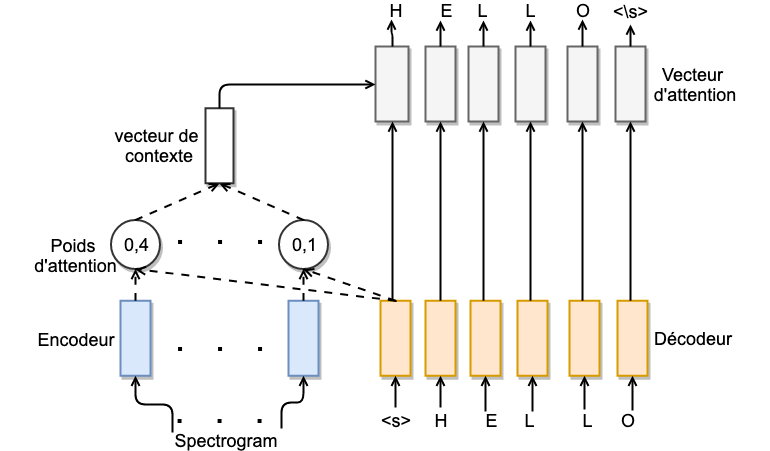
\includegraphics[height=205pt,width=365pt]{images/chap3/Att.png}
    \caption{Mécanisme d'attention}
    \label{atn}
\end{figure}

Nous pourrions introduire ce mécanisme en ajoutant une couche d'attention au modèle de base qui permettrait de relier les sorties de l'encodeur à celles du décodeur. Nous pensons que cette approche pourrait présenter un meilleur apprentissage. La figure \ref{archi_atn} schématise l'architecture d'un tel modèle.

\begin{figure}[H]
    \centering
    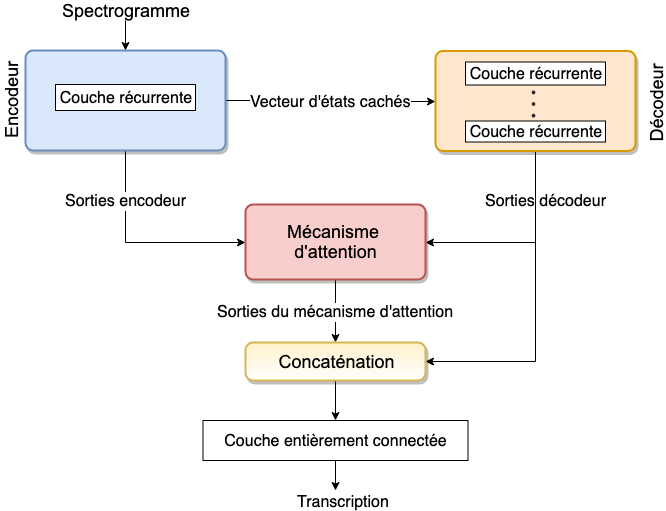
\includegraphics[width=320pt, height=240pt]{images/chap3/Attention.png}
    \caption{Architecture d'un modèle End-To-End avec mécanisme d'attention}
    \label{archi_atn}
\end{figure}

% Comme le montre la figure \ref{archi_atn}, le modèle de base se compose des modules suivants :
% \begin{itemize}
%     \item \textbf{Encodeur} : composé d'une couche récurrente et renvoie les vecteurs Hidden State mais aussi l'output de l'encodeur qui sera utilisé par la couche d'attention.
%     \item \textbf{Décodeur} : composé de plusieurs couches récurrentes où la première couche prend comme entrée les vecteurs Hidden State produits en sortie de l'encodeur.
%     \item \textbf{Mécanisme d'attention} : prend en entrée les sorties de l'encodeur et les sortie du décodeur pour effectuer un alignement des timesteps de l'entrée audio avec les timesteps de la transcription.
%     \item \textbf{Couche Fully Connected} : Dernière couche du modèle, prend en entrée l'output du décodeur.
% \end{itemize}

Pour clore, nous pouvons dire que la réalisation de ce projet nous a permis de maîtriser des domaines importants de l'intelligence artificielle. À travers ce travail nous avons : 
\begin{itemize}
    \item maîtrisé les principes de la reconnaissance automatique de la parole mais aussi les principes des systèmes de questions-réponses avec de potentielles applications très importantes que ce soit pour le web, applications mobiles ou autres plateformes, et
    \item approfondi nos connaissances en apprentissage automatique et maîtrisé de nouvelles approches plus flexibles et plus performantes nous permettant ainsi d'appréhender un grand éventail de problématiques d'intelligence artificielle. \\
\end{itemize}

En plus des compétences informatiques acquises, nous avons appris à gérer un projet, à rédiger un mémoire de qualité et à travailler en équipe tout en respectant les différentes conventions qui sont utilisées dans le monde professionnel. Au terme de ce projet, les enseignements s'avèrent être précieux et nous seront utiles tout au long de nos parcours respectifs.   






%%% References %%%
 \newpage
 \pagenumbering{gobble} 
 \bibliographystyle{apalike} 
 \bibliography{ref}
 
  \appendix
 \chapter{Documentation }
 \section{models}
\subsection{Speech\_API}
    ASER\_system est la fonction principale de ce module qui contient un système de reconnaissance de la parole pour la langue arabe, ce dernier peut être intégré à n'importe quelle application. 
    
\subsection{Apprentissage}
    \subsubsection{encoder\_decoder}
    Nous commençons par vous présentez 4 types d'encodeurs :
    \begin{enumerate}
        \item \textbf{Encodeur LSTM :} 
            \begin{tcolorbox}
                get\_encoder\_states\_LSTM(encoder\_inputs, latent\_dim, return\_sequences=False)
            \end{tcolorbox}
            Fonction implémentant un encodeur avec une couche LSTM \\
        \item \textbf{Encodeur GRU :} 
            \begin{tcolorbox}
            get\_encoder\_states\_GRU(encoder\_inputs, latent\_dim, return\_sequences=False)
            \end{tcolorbox}
            Fonction implémentant un encodeur avec une couche GRU \\
        \item \textbf{Encodeur Bi-LSTM :}
            \begin{tcolorbox}
            encoder\_bi\_LSTM(encoder\_inputs, latent\_dim, return\_sequences=False)
            \end{tcolorbox}
            Fonction implémentant un encodeur avec une couche LSTM  bidirectionnelle \\
        \item \textbf{Encodeur Bi-GRU :}
            \begin{tcolorbox}
            encoder\_bi\_GRU(encoder\_inputs, latent\_dim, return\_sequences=False)
            \end{tcolorbox}
            Fonction implémentant un encodeur avec un couche GRU bidirectionnelle \\
    \end{enumerate}
    Toutes ces fonctions ont les mêmes arguments en entrée et renvoie la même chose en sortie. \\
    \textbf{Arguments} 
    \begin{itemize}
        \item encoder\_inputs : 3D Numpy Array, les données en entrèe pour l'encodeur.
        \item latent\_dim : Entier positif, dimensionnalité de l'espace de sortie.
        \item return\_sequences=False : Booléen. Indique s'il faut renvoyer la dernière sortie de la séquence de sortie ou la séquence complète du LSTM.
    \end{itemize}
    \textbf{Retourne} 
    \begin{itemize}
        \item encoder\_states : le vecteur d'états cachés renvoyé par la couche LSTM
    \end{itemize}  
    Dans ce qui suit, nous présentons 4 types de décodeurs :
    \begin{enumerate}
        \item \textbf{Décodeur LSTM :} 
            \begin{tcolorbox}
            get\_decoder\_outputs\_LSTM( encoder\_inputs, latent\_dim, return\_sequences=False)
            \end{tcolorbox}
            Fonction implémentant un décodeur avec trois couches LSTM  \\
        \item \textbf{Décodeur GRU :}  
            \begin{tcolorbox}
            get\_decoder\_outputs\_GRU(encoder\_inputs, latent\_dim, return\_sequences=False)
            \end{tcolorbox}
            Fonction implémentant un décodeur avec trois couches GRU \\
        \item \textbf{Décodeur Bi-LSTM :}  
            \begin{tcolorbox}
            decoder\_for\_bidirectionnal\_encoder\_LSTM(encoder\_inputs, latent\_dim, return\_sequences=False)
            \end{tcolorbox}
            Fonction implémentant un décodeur avec trois couches LSTM bidirectionnelles \\
        \item \textbf{Décodeur Bi-GRU :} 
            \begin{tcolorbox}
            decoder\_for\_bidirectionnal\_encoder\_GRU(encoder\_states, decoder\_inputs, latent\_dim)
            \end{tcolorbox} 
            Fonction implémentant un décodeur avec trois couches GRU bidirectionnelles \\
    \end{enumerate}
    Toutes ces fonctions ont les mêmes arguments en entrée et renvoie la même chose en sortie.\\
        \textbf{Arguments} \\
        \begin{itemize}
            \item encoder\_inputs : 3D Numpy Array, les données en entrèe pour l'encodeur.
            \item decoder\_inputs : 3D Numpy Array. Les données en entrée du décodeur
            \item latent\_dim : Entier positif, dimensionnalité de l'espace de sortie.
        \end{itemize}
        \textbf{Retourne}
        \begin{itemize}
            \item decoder\_states : le vecteur d'états cachés renvoyé par la couche LSTM
            \item decoder\_outputs : 3D Numpy array. Représente le résultat obtenu par le décodeur
        \end{itemize}
    
    
    \subsubsection{baseline\_model}
    \begin{enumerate}
        \item \textbf{Modèle Baseline en utilisant des couches GRU} 
            \begin{tcolorbox}
                train\_baseline\_seq2seq\_model\_GRU(mfcc\_features, target\_length, latent\_dim, word\_level)
            \end{tcolorbox}
            Modèle de base implémenté en utilisant des couches GRU pour l'encodeur ainsi que le décodeur \\
        \item \textbf{Modèle Baseline en utilisant des couches GRU bidirectionnelles}
            \begin{tcolorbox}
            train\_bidirectional\_baseline\_seq2seq\_model\_GRU(encoder\_inputs, latent\_dim, return\_sequences=False)
            \end{tcolorbox}
            Modèle de base implémenté en utilisant des couches GRU bidirectionnelles pour l'encodeur ainsi que le décodeur \\
        \item \textbf{Modèle Baseline en utilisant des couches LSTM} 
            \begin{tcolorbox}
            train\_baseline\_seq2seq\_model\_LSTM(encoder\_inputs, latent\_dim, return\_sequences=False)
            \end{tcolorbox}
            Modèle de base implémenté en utilisant des couches LSTM pour l'encodeur ainsi que le décodeur \\
        \item \textbf{Modèle Baseline en utilisant des couches LSTM  bidirectionnelles} 
            \begin{tcolorbox}
            train\_bidirectional\_baseline\_seq2seq\_model\_LSTM(encoder\_inputs, latent\_dim, return\_sequences=False)
            \end{tcolorbox}
            Modèle de base implémenté en utilisant des couches LSTM bidirectionnelles pour l'encodeur ainsi que le décodeur \\
            \textbf{Arguments} 
            \begin{itemize}
                \item mfcc\_features : 3D Numpy Array
                \item target\_length : Entier positif, taille de l'output du décodeur
                \item latent\_dim : Entier positif, dimensionnalité de l'espace de sortie.
                \item word\_level : Booléen, 0 si les transcriptions sont basées caractères, 1 sinon.
            \end{itemize}
            \textbf{Retourne} 
            \begin{itemize}
                \item model : Définit une instance de model séquence à séquence 
                \item encoder\_states : le vecteur d'états cachés renvoyé par la couche LSTM
            \end{itemize}
    \end{enumerate}

    \subsubsection{cnn\_based\_model}
    \begin{enumerate}
        \item \textbf{Modèle avec couche convolutionnelles et Encodeur/Décodeur avec des couches GRU}  
            \begin{tcolorbox}
                train\_cnn\_seq2seq\_model\_GRU(mfcc\_features, target\_length, latent\_dim, word\_level)
            \end{tcolorbox}
            Modèle implémenté en utilisant des couches GRU pour l'encodeur ainsi que le décodeur \\
        \item \textbf{Modèle avec couche convolutionnelles et Encodeur/Décodeur avec des couches GRU bidirectionnelles} 
            \begin{tcolorbox}
            train\_bidirectional\_baseline\_seq2seq\_model\_GRU(encoder\_inputs, latent\_dim, return\_sequences=False)
            \end{tcolorbox}
            Modèle de base implémenté en utilisant des couches GRU bidirectionnelles pour l'encodeur ainsi que le décodeur \\
        \item \textbf{Modèle avec couche convolutionnelles et Encodeur/Décodeur avec des couches LSTM} 
            \begin{tcolorbox}
            train\_baseline\_seq2seq\_model\_LSTM(encoder\_inputs, latent\_dim, return\_sequences=False)
            \end{tcolorbox}
            Modèle de base implémenté en utilisant des couches LSTM pour l'encodeur ainsi que le décodeur \\
        \item \textbf{Modèle avec couche convolutionnelles et Encodeur/Décodeur avec des couches LSTM  bidirectionnelles}
            \begin{tcolorbox}
            train\_bidirectional\_baseline\_seq2seq\_model\_LSTM(encoder\_inputs, latent\_dim, return\_sequences=False)
            \end{tcolorbox}
            Modèle de base implémenté en utilisant des couches LSTM bidirectionnelles pour l'encodeur ainsi que le décodeur \\
            \textbf{Arguments} 
            \begin{itemize}
                \item mfcc\_features : 3D Numpy Array
                \item target\_length : Entier positif, taille de l'output du décodeur
                \item latent\_dim : Entier positif, dimensionnalité de l'espace de sortie.
                \item word\_level : Booléen, 0 si les transcriptions sont basées caractères, 1 sinon.
            \end{itemize}
            \textbf{Retourne} 
            \begin{itemize}
                \item model : Définit une instance de model séquence à séquence 
                \item encoder\_states : le vecteur d'états cachés renvoyé par la couche LSTM
            \end{itemize}
    \end{enumerate}
    
    
    \subsubsection{model\_callback}
    \begin{tcolorbox}
    ModelSaver(model\_name, model\_path, encoder\_states, drive\_instance, word\_level=True, output\_length=16)
    \end{tcolorbox}
    Classe permettant de sauvegarder le modèle après cheque itération lors de l'apprentissage \\
    \textbf{Arguments} 
    \begin{itemize}
        \item model\_name : chaine de caratères, le nom du modèle.
        \item model\_path : chaine de caratères, le chemin vers le modèle.
        \item encoder\_states
        \item word\_level : Booléen, 0 si les transcriptions sont basées caractères, 1 sinon.
        \item output\_length : entier positif, taille de l'output.
    \end{itemize}
    \textbf{Méthodes}
    \begin{itemize}
        \item on\_epoch\_end(epoch, logs=None)
    \end{itemize}
    
    \subsubsection{train\_model}
    \begin{tcolorbox}
    Seq2SeqModel(latent\_dim=300, epochs=50, model\_architecture=5, data\_generation=True, word\_level=False)
    \end{tcolorbox}
    Classe permettant de faire le traitement nécessaire pour l'apprentissage d'un modèle seéquence à séquence.\\
    \textbf{Arguments}
    \begin{itemize}
        \item latent\_dim : entier positif, 
        \item epochs : entier positif, 
        \item model\_architecture : entier positif
        \item data\_generation : Booléen, 
        \item word\_level : Booléen, 0 si les transcriptions sont basées caractères, 1 sinon.
    \end{itemize}
    \textbf{Méthodes}
    \begin{itemize}
        \item test\_model()
        \item train\_model()
        \item validation\_generator()
        \item split\_data\_generator\_dict\_test()
        \item split\_data\_generator\_dict(batch\_size)
        \item split\_data\_generator\_dict\_word\_level(batch\_size)
        \item split\_data\_generator\_dict\_word\_level\_test()
        \item get\_test\_data(audio\_file, transcripts\_file)
        \item get\_data(audio\_file, transcripts\_file)
    \end{itemize}
    
    % \subsubsection{test\_model}
    
    \subsubsection{plot\_performance}
    \begin{tcolorbox}
    plot\_train\_loss\_acc(model\_hist\_path, word\_level)
    \end{tcolorbox}
    Fonction permettant d'afficher les courbes d'appentissage et de test (loss et accuracy) \\
    \textbf{Arguments} 
    \begin{itemize}
        \item model\_hist\_path : le chemin vers l'historique du modèle
        \item word\_level : Booléen, 0 si les transcriptions sont basées caractères, 1 sinon.
    \end{itemize}

    
    \subsubsection{char\_inference}
    \begin{tcolorbox}
    Char\_Inference()
    \end{tcolorbox}
    Fonction permeettant l'inférence en utilisant un modèle basé caractères. \\
    \subsubsection{word\_inference}
    \begin{tcolorbox}
    Word\_Inference(model\_path, latent\_dim)
    \end{tcolorbox}
    Fonction permeettant l'inférence en utilisant un modèle basé mots. \\
    \textbf{Arguments} 
    \begin{itemize}
        \item model\_path : chaine de caractères, chemain vers le modèle choisi.
        \item latent\_dim : entier positif, 
    \end{itemize}
    
    \subsubsection{word\_correction}
    \begin{tcolorbox}
    correct\_word(word\_to\_correct)
    \end{tcolorbox}
    Fonction permettant la correction d'un mot en utilisant un modèle de language. \\
    \textbf{Arguments}
    \begin{itemize}
        \item word\_to\_correct : chaine de caractères, le mot à corriger.
    \end{itemize}
    

\section{data}
    \subsection{Dataset generation}
    \subsubsection{audio\_transcript\_map}
    \begin{tcolorbox}
    map\_audio\_transcripts()
    \end{tcolorbox}
    Fonction permettant de mapper chaque audio avec sa transcription.
    \subsubsection{parse\_xml}
    \begin{tcolorbox}
    generate\_transcriptions\_file(transcriptions\_desc, output\_path)
    \end{tcolorbox}
    Fonction permettant la génération d'un fichier des transcriptions à partir d'un XML \\
    \textbf{Arguments}
    \begin{itemize}
        \item transcriptions\_desc
        \item output\_path
    \end{itemize}
    
    \subsubsection{split\_audio}
    \begin{tcolorbox}
    split\_audio(audio\_entry, transcriptions\_desc, audio\_output\_dir)
    \end{tcolorbox}
    Fonction permettant de diviser un audio en plusieurs sous-audio. \\
    \textbf{Arguments}
    \begin{itemize}
        \item audio\_entry
        \item transcriptions\_desc
        \item audio\_output\_dir
    \end{itemize}
    \subsubsection{parse\_dataset}
    \begin{tcolorbox}
    generate\_dataset()
    \end{tcolorbox}
    Fonction permettant la génération d'un fichier Pickle contenant toutes les informations nécessaire et les données du dataset 
    
    \subsection{pré-traitement des données}
    \subsubsection{normalisation}
    \begin{tcolorbox}
    normalize\_encoder\_input(dataset)
    \end{tcolorbox}
    Fonction permettant la normalisation des entrés de l'encodeur \\
    \textbf{Arguments}
    \begin{itemize}
        \item dataset
    \end{itemize}
    % \subsubsection{clean\_audio}
    \subsubsection{transcript\_preprocessing}
    \begin{tcolorbox}
    transcript\_preprocessing(transcription, special\_characters\_table)
    \end{tcolorbox}
    Fonction permettant de faire le pré-traitement des transcriptions \\
    \textbf{Arguments}
    \begin{itemize}
        \item transcription
        \item special\_characters\_table
    \end{itemize}
    % \subsubsection{transcript\_content}
    % \subsubsection{transcript\_encoding}
    % \subsubsection{prepare\_dataset}
\section{lib}
    \subsection{AudioInput}
    \begin{tcolorbox}
    AudioInput(path, transcript)
    \end{tcolorbox}
    Classe permettant de représenter un audio, ses caractéristiques ainsi que sa transcription \\
    \textbf{Arguments}
    \begin{itemize}
        \item path
        \item transcript
    \end{itemize}
    \subsection{Transcript}
    \begin{tcolorbox}
    Transcript(start\_time, end\_time, content)
    \end{tcolorbox}
    \textbf{Arguments}
    \begin{itemize}
        \item start\_time
        \item end\_time
        \item content
    \end{itemize}
\section{utils}
    \subsection{character\_convesion}
    \begin{enumerate}
        \item Conversion d'une phrase de la langue arabe au buckwalter :
        \begin{tcolorbox}
        arabic\_to\_buckwalter(arabic\_sentence)
        \end{tcolorbox}
        \textbf{Arguments}
        \begin{itemize}
            \item arabic\_sentence
        \end{itemize}
        \item Conversion d'une phrase du buckwalter à l'arabe:
        \begin{tcolorbox}
        buckwalter\_to\_arabic(buckwalter\_sentence)
        \end{tcolorbox}
        \textbf{Arguments}
        \begin{itemize}
            \item buckwalter\_sentence
        \end{itemize}
        \item Conversion des chiffres en lettres :
        \begin{tcolorbox}
        convert\_numeral\_to\_written\_number(number)
        \end{tcolorbox}
        \textbf{Arguments}
        \begin{itemize}
            \item number
        \end{itemize}
        \item Conversion ...
        \begin{tcolorbox}
        numerical\_to\_written\_numbers\_table(inf\_number=0, sup\_number=10001)
        \end{tcolorbox}
        \textbf{Arguments}
        \begin{itemize}
            \item inf\_number=0
            \item sup\_number=10001
        \end{itemize}
    \end{enumerate}

    \subsection{pickle\_management}
    \begin{tcolorbox}
    generate\_pickle\_dataset(threshold)
    \end{tcolorbox}
    \textbf{Arguments}
    \begin{itemize}
        \item threshold
    \end{itemize}
    % \subsection{utils}
\section{etc}
    Toutes les constantes sont enregistrées dans settings, nous retrouvant :
    \begin{itemize}
        \item DATA\_PATH : Chemin vers le dossier \textit{data}.
        \item PICKLE\_FILE\_PATH : Chemin vers le fichier pickle.
        \item PICKLE\_PARTITIONS\_PATH : Chemin vers le dossier \textit{partitions}.
        \item PICKLE\_PAD\_FILE\_PATH 
        \item GENERATED\_DATA\_PATH : Chemin vers le dossier generated\_data.
        \item GENERATED\_DATA\_WAV\_PATH : Chemin vers le dossier wav de generated\_data.
        \item GENERATED\_DATA\_TRANSCRIPTS\_PATH : Chemin vers le dossier transcripts de generated\_data.
        \item DISTINCT\_CHARACTERS\_PATH : Chemin vers le fichier contenant les caractères distincts du corpus.
        \item NORMALIZATION\_PATH : Chemin vers le dossier \textit{normalisation}
        \item TRAINED\_MODELS\_PATH : Chemin vers le dossier \textit{trained\_models}
        \item DATASET\_SPLIT\_PATH : Chemin vers le dossier \textit{dataset\_split}
        \item DATASET\_SPLIT\_TRAIN\_PATH : Chemin vers le dossier \textit{train } de \textit{dataset\_split}
        \item DATASET\_SPLIT\_TEST\_PATH : Chemin vers le dossier \textit{test} de \textit{dataset\_split}
        \item MFCC\_FEATURES\_LENGTH 
        \item CHARACTER\_SET : Ensemble de caractères du corpus.
        \item WORD\_SET : Ensemble des mots du corpus.
        \item LONGEST\_WORD\_LENGTH : Taille du plus grand mot.
        \item WORD\_TARGET\_LENGTH 
        \item TOTAL\_SAMPLES\_NUMBER
    \end{itemize}
 
 
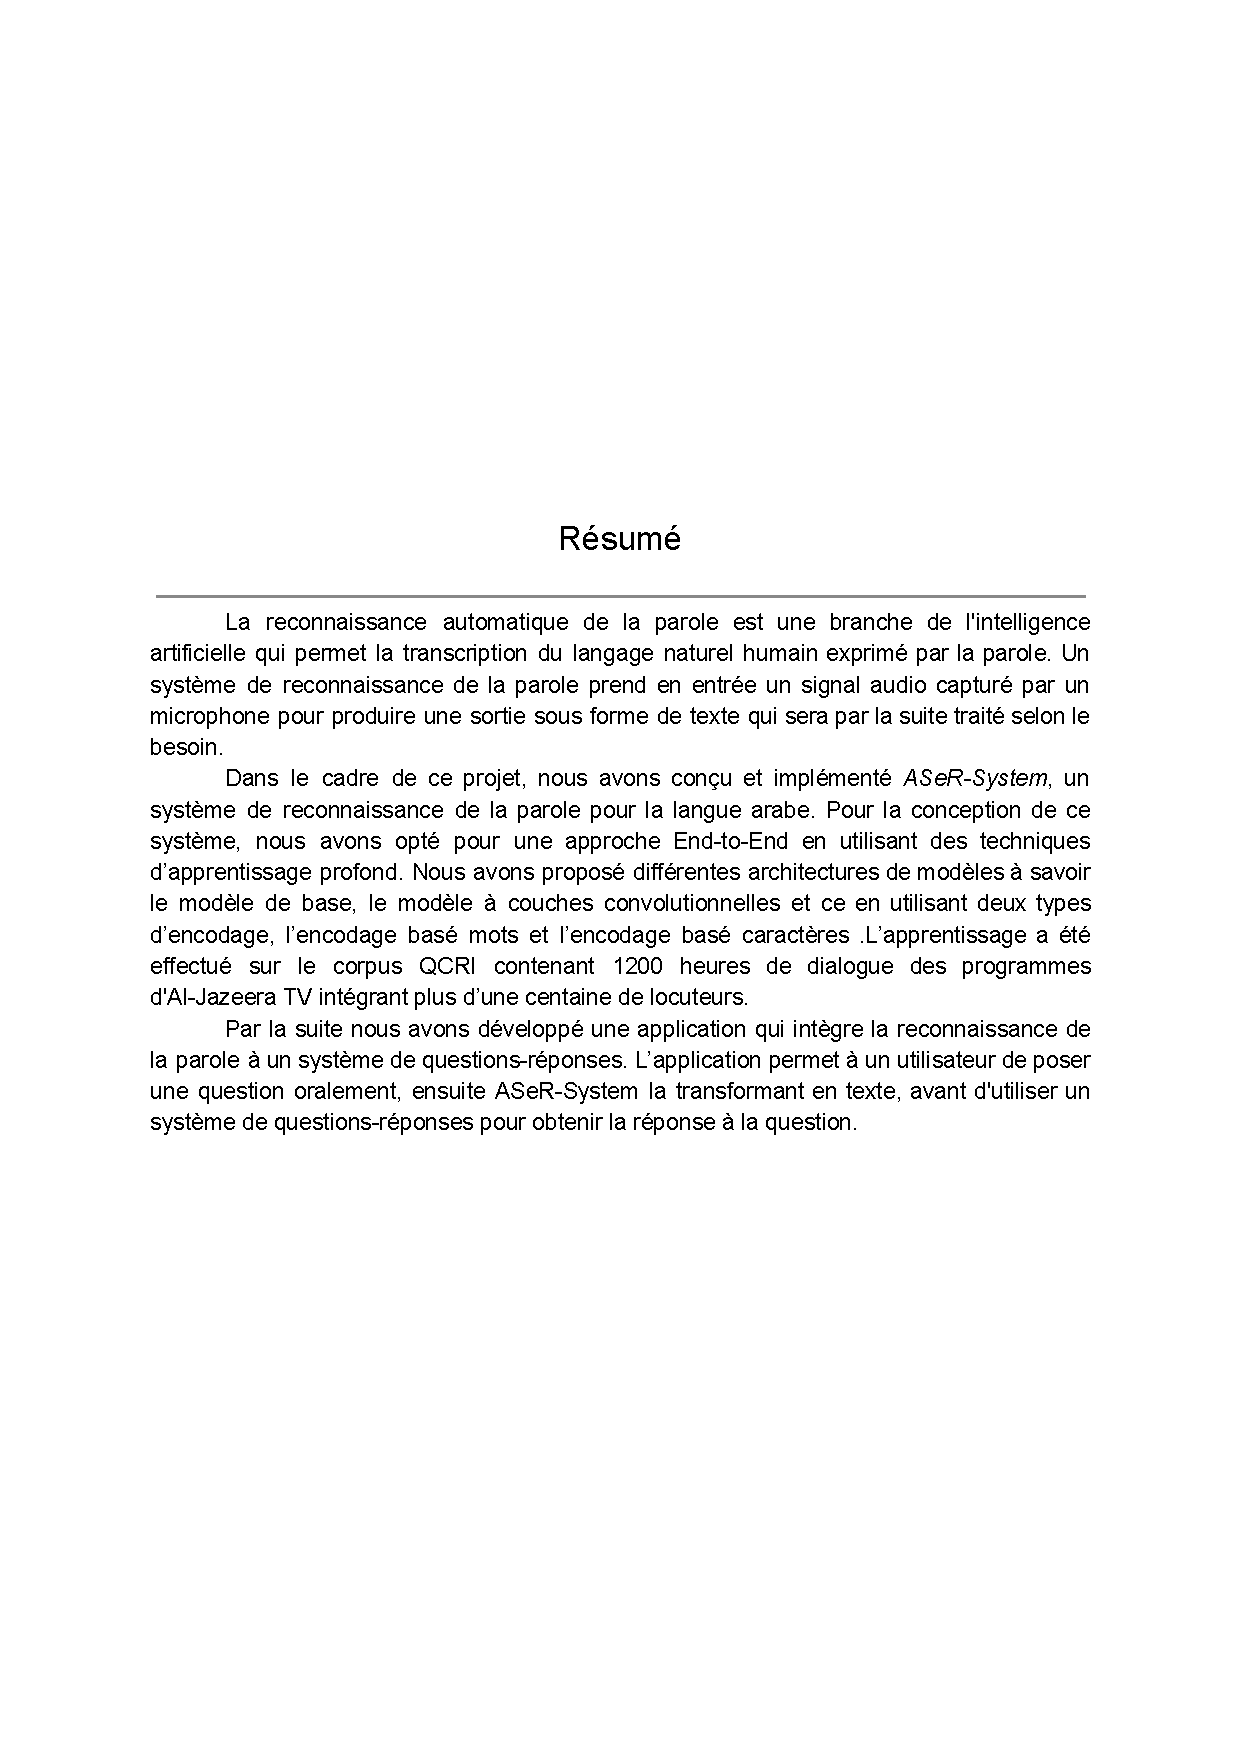
\includepdf[pages=1]{other/abstract.pdf}
\includepdf[pages=2]{other/abstract.pdf}
\includepdf[pages=3]{other/abstract.pdf}
\end{document}
%~~~END~~~%